% Abschlussarbeit am Ende der Oberschule
% Facharbeit zum parallelen Programmierparadigma
% Thomas Mittermair
% Oberschulzentrum J. Ph. Fallmerayer Brixen

% include file containing tex configurations
% Abschlussarbeit am Ende der Oberschule
% Facharbeit zum parallelen Programmierparadigma
% Thomas Mittermair
% Oberschulzentrum J. Ph. Fallmerayer Brixen

% define document class
\documentclass[11pt, a4paper, titlepage, twoside, german]{report}

% include required packages
\usepackage{fancyhdr}
\usepackage{graphicx}
\usepackage[ngerman, english]{babel}
\usepackage[utf8]{inputenc}
\usepackage[T1]{fontenc}
%\usepackage{times}
\usepackage{lmodern}
\usepackage{url}
\usepackage{appendix}
\usepackage[nottoc,notlot,notlof]{tocbibind}
\usepackage{listings}
\usepackage[pdftex, pdfauthor={Thomas Mittermair}, pdftitle={Paralleles Programmierparadigma}]{hyperref}	% Set title and author used in the pdf meta data.
\usepackage{microtype} % tweak spacing and sizing so everything fits nicely
\usepackage{amsmath} % Für die Darstellung von mathematischen, stückweise definierten Funktionen.
\usepackage[style=numeric, backend=bibtex]{biblatex} 
\addbibresource{Literatur.bib} % Zuweisung der *.bib bei Biblatex.

% specify margins for two-sided print
\oddsidemargin 3cm
\evensidemargin 1cm
\textwidth 12cm

% define header format
\fancypagestyle{plain}{
	\fancyhf{} % Clear header/footer
	\fancyhead[LE,RO]{\leftmark}
	\fancyfoot[LE,RO]{\textit{Paralleles Programmierparadigma}}
	\fancyfoot[RE,LO]{\thepage}
	\fancyfoot[CE, CO]{}
}
\pagestyle{plain} % Set page style to plain.

\headheight 26pt
\renewcommand{\headrulewidth}{0.3pt}
\renewcommand{\footrulewidth}{0.3pt}

% define style for appendix header
\newcommand{\appendixheader}{ % specify header for appendix
    \fancyhf{}
    \fancyhead[LE, RO]{APPENDIX \rightmark}
    \fancyfoot[LO, RE]{Name 1, Name 2}
    \fancyfoot[RO, LE]{\thepage}
}

% code for creating empty pages
% no headers on empty pages before new chapter
\makeatletter
\def\cleardoublepage{\clearpage\if@twoside \ifodd\c@page\else
    \hbox{}
    \thispagestyle{empty}
    \newpage
    \if@twocolumn\hbox{}\newpage\fi\fi\fi}
\makeatother \clearpage{\pagestyle{empty}\cleardoublepage}

\setcounter{secnumdepth}{6} % setting level of numbering

\renewcommand{\arraystretch}{1.5} % Der Abstand zwischen den Zeilen einer Tabelle wird angepasst.

% Nun werden die Zeichen gesetzt, bei welchen Zeilenumbrüche bei URLs eingefügt werden können (von Latex automatisch).
\usepackage{url}
\usepackage{breakurl}
\usepackage{hyperref}
\def\UrlBreaks{\do\/\do-\do\_} % Die URL kann nur bei "/", "-" und "_" getrennt werden.

% start document
\begin{document}
	\parindent 0cm 
	\selectlanguage{german}
	
	\hypersetup{	% Set title and author used in the pdf meta data.
		pdftitle={Paralleles Programmierparadigma},
		pdfauthor={Thomas Mittermair}
	}	
	
	\title{Paralleles Programmierparadigma}
	\author{Thomas Mittermair}
	\date{\today}
	\pagenumbering{Roman}

	% Abschlussarbeit am Ende der Oberschule
% Facharbeit zum parallelen Programmierparadigma
% Thomas Mittermair
% Oberschulzentrum J. Ph. Fallmerayer Brixen

\begin{titlepage}
	\begin{center}
		% insert Fallmerayer-logo
		
\includegraphics[height=50mm]{Abbildungen/Fallmerayer_Logo.jpg} \\[3mm]
		\vspace{1cm}

		\begin{large}
			Oberschulzentrum J. Ph. Fallmerayer Brixen\\[5mm]
			Technologische Fachoberschule (TFO)\\[2mm]
			Fachrichtung Informatik und Telekommunikation\\
			Schwerpunkt Informatik\\[20mm]
		\end{large}

		{\LARGE Paralleles Programmierparadigma\\[9mm]}
		Abschlussarbeit am Ende der Oberschule\\[2mm]
		Facharbeit aus Technologien und Planung von informatischen Systemen und Telekommunikationssystemen (TP)\\[2mm]
		Schuljahr 2017/18\\[9mm]

		Thomas Mittermair\\[2mm]
		Klasse 5BT\\[9mm]

		Betreut von\\
		Prof. Alexander Larcher\\[7mm]

		Brixen, Italien,\\
		am \today
	\end{center}
\end{titlepage}
	\clearpage
	
	% Abschlussarbeit am Ende der Oberschule
% Facharbeit zum parallelen Programmierparadigma
% Thomas Mittermair
% Oberschulzentrum J. Ph. Fallmerayer Brixen

\renewcommand{\abstractname}{Abstract}

\begin{abstract}
	Das 21. Jahrhundert steht im Zeichen der Beschleunigung. Immer mehr Menschen führen ein immer schnelleres Leben, dies trifft auch auf das digitale Dasein zu. Die Benutzer verlangen immer schnellere Reaktionszeiten von Programmen und Webseiten und sind keineswegs gewillt zu warten.\\
	Das Problem hierbei liegt darin, dass Rechner bestimmten physikalischen Grenzen unterworfen sind, die eine weitere Beschleunigung ab einem gewissen Punkt unmöglich machen. An dieser Stelle kommt die Parallelisierung ins Spiel. Sie ist ein Ansatz, der zu einem Geschwindigkeitsgewinn führen kann, ohne dabei von der Weiterentwicklung der Hardware abhängig zu sein. Die Idee besteht darin, die großen zu berechnenden Probleme aufzuteilen und mehrere Komponenten \textit{parallel} daran arbeiten zu lassen. Dieser Ansatz der Programmierung wird in der Informatik als \textit{Paralleles Programmierparadigma} bezeichnet. Auch wenn der Ansatz zunächst trivial klingt, so verbergen sich dahinter trotzdem ungeahnte Probleme, die es zu lösen gilt.\\
	Aus diesem Grund ist es das Ziel dieser Arbeit, zunächst die theoretischen Grundlagen der Parallelisierung zu legen und dann verschiedene Ansätze anhand eines praktischen Beispiels zu vergleichen.
\end{abstract}
	\clearpage

	\setcounter{page}{1}
	
	\setcounter{tocdepth}{2} % set depth of the table of contents
	\tableofcontents
	\cleardoublepage
	
	\pagenumbering{arabic}
	\setcounter{page}{1}
	
	% Abschlussarbeit am Ende der Oberschule
% Facharbeit zum parallelen Programmierparadigma
% Thomas Mittermair
% Oberschulzentrum J. Ph. Fallmerayer Brixen

\chapter{Einleitung und Motivation}

	\section{Einführung in die Problematik der Parallelisierung}

		Der Begriff der \textit{Parallelität} existiert nicht nur im Bereich der Informatik, sondern vor allem im Alltag und in der Natur ist selbiger oft vorzufinden und somit allgegenwärtig. Um zu begreifen, worum es sich bei Parallelität handelt, muss zunächst klargestellt werden, worin der Unterschied zwischen Sequentialität und Parallelität liegt.

		\subsection{Begriffe der Sequentialität und Parallelität}

			Die Ausdrücke \textit{Sequentialität} und \textit{Parallelität} stellen Schlüsselbegriffe im Zusammenhang mit dieser Arbeit dar. Der Online-Duden gibt für diese beiden Begriffe die nun folgenden Definitionen.
			
			\begin{description}
			  \item[Sequentialität]
				  Der Begriff \textit{Sequentialität} hängt eng mit dem Adjektiv \textit{sequenziell} zusammen. Vorgänge, die sequenziell ablaufen, spielen sich aufeinander folgend und der Reihe nach ab. \cite{SequentiellDuden}
			  \item[Parallelität]
				  Der Begriff \textit{Parallelität} hängt eng mit dem Adjektiv \textit{parallel} zusammen. Vorgänge, die parallel ablaufen, spielen sich gleichzeitig und synchron ab. \cite{ParallelDuden}
			\end{description}

			\subsubsection{Sequentialität und Parallelität im Alltag und in der Natur}
			
				Jeder Mensch ist, oft ohne davon Kenntnis zu nehmen, täglich mit sequentiellen und parallelen Vorgängen und Abläufen konfrontiert. Ein alltägliches Beispiel für Sequentialität ist der Begriff von Zeit, denn eine Sekunde vergeht erst, sobald die vorherige Sekunde vollkommen abgelaufen ist. Zeit läuft somit vollkommen sequentiell ab, wodurch das Kausalitäts-Prinzip, also das Prinzip von Ursache und Wirkung, erst möglich wird, denn hätte die Zeit diese Eigenschaft nicht, so wären Ursache und Wirkung nicht klar voneinander unterscheidbar. Folglich geschieht in der Natur nichts ohne Grund, und das bedeutet wiederum, dass es zu jedem beliebigen Ereignis ein anderes Ereignis gibt, das in der Vergangenheit liegt und das nachfolgende Ereignis hervorruft. \cite{Kausalitaet} Viele Vorgänge in der Natur laufen hingegen parallel ab. Beispielsweise findet stets eine simultane Weiterentwicklung statt, denn jeder Mensch und auch jede Pflanze entwickeln sich gleichzeitig, und nicht nacheinander, weiter. \cite{ParaProgLoogen}
				
			\subsubsection{Sequentialität und Parallelität in der Informatik}
				\label{SequUndParaInformatik}
				
				Die Informatik ist eine Wissenschaft, die in vielen Bereichen das Ziel verfolgt, Objekte und auch Abläufe der realen Welt auf Ebene von Rechnern möglichst realitätsgetreu nachzubilden. Ein informatisches Modell der Wirklichkeit soll folglich so nahe wie möglich an die zu modellierende Begebenheit herankommen. Ein in diesem Zusammenhang oft genanntes Beispiel ist das objektorientierte Programmierparadigma. Dabei werden Objekte der realen Welt durch Datenstrukturen im Computer nachgeahmt. Dies erlaubt es, Sachverhalte in der Realität nahezu direkt und ohne große Abänderungen in einer objektorientierten Programmiersprache zu modellieren. \cite{Objektorientierung} Ähnliches gilt für die Sequentialität und Parallelität in der Informatik. Um zu verstehen, wie diese beiden Gegensätze in der Informatik zusammenhängen und realisiert werden, muss zunächst erläutert werden, wie ein Prozessor Befehle abarbeitet.
				
				\begin{description}
			  		\item[Ausführungsschema eines Prozessors]
						Der Prozessor, auch CPU (Central Processing Unit) genannt, ist das Herzstück eines Rechners. Er ist die Komponente, welche für die Ausführung und Abarbeitung der Befehle zuständig ist. Ein Prozessor kann dabei im Normalfall, also sofern er nur aus einem Kern besteht, nur eine Operation zugleich ausführen. Diese Eigenschaft leitet sich vom Schema ab, nach welchem die Mehrheit aller im Moment auf dem Markt befindlichen CPUs arbeiten. Dabei handelt es sich um den \textit{Von-Neumann-Zyklus}, allgemeiner auch als \textit{Befehlszyklus} bekannt.
						Die Abarbeitung eines Befehls geschieht dabei meist nach dem folgenden Schema:
						
						\begin{enumerate}
							\item \textbf{Instruction-Fetch-Phase (IF), Befehlholungs-Phase}: In dieser Phase wird der Befehlscode vom Hauptspeicher in ein Register des Prozessors geladen.
							\item \textbf{Instruction-Decode-Phase (ID), Befehldekodierungs-Phase}: Der in ein Register geladene Befehl wird nun decodiert, um den Befehl weiterverarbeiten zu können. In dieser Phase wird der Befehl folglich analysiert, um Informationen zur Art des Befehls sowie zu Art und Anzahl der beteiligten Operanden und weitere Details zu ermitteln.
							\item \textbf{Fetch-Operands-Phase (FO), Operandennachladungs-Phase}: In dieser Phase werden die Operanden, welche zur Abarbeitung des Befehls notwendig sind, in die Register nachladen. Bei Befehlen ohne Operanden bleibt diese Phase leer, da sie in diesem Fall nicht benötigt wird. Die Fetch-Operands-Phase kann auch als Unterphase der Instruction-Decode-Phase betrachtet werden, da die Operanden, welche in der Instruction-Decode-Phase ermittelt wurden, in dieser Phase aus dem Hauptspeicher in die Register geladen werden.
							\item \textbf{Execute-Phase (EX), Befehlausfühungs-Phase}: In dieser Phase kann der Befehl nun, beispielsweise unter Verwendung des Rechenwerkes, ausgeführt werden. Hierbei wird der geladene Befehl unter Verwendung der geladenen Operanden (falls vorhanden) abgearbeitet.
							\item \textbf{Write-Back-Phase (WB), Resultat-Rückschreibungs-Phase}: In dieser Phase werden die Ergebnisse aus der Execute-Phase in den Speicher (z.B. in ein anderes Register oder auch in einen externen Speicher) zurückgeschrieben. Bei Befehlen ohne Resultat bleibt diese Phase leer, da sie nicht benötigt wird.
						\end{enumerate}
						
						Jeder einzelne Befehl durchläuft dieses Schema, das bedeutet, nachdem ein Befehl die Write-Back-Phase abgeschlossen hat, kann der nächste Befehl mit der Instruction-Fetch-Phase beginnen. \cite{PhasenBefehlsbearbeitung} \cite{FunktionsweiseComputersysteme}\\
						
						Diese Sequentialität des Befehlszyklus soll nun an Hand eines Beispiels der Abarbeitung von drei Befehlen verdeutlicht werden.
						Die Abbildung \ref{fig:BefehlszylusOhnePipelining} soll diesen Vorgang grafisch veranschaulichen.
						
						\begin{figure}
							\centering	
							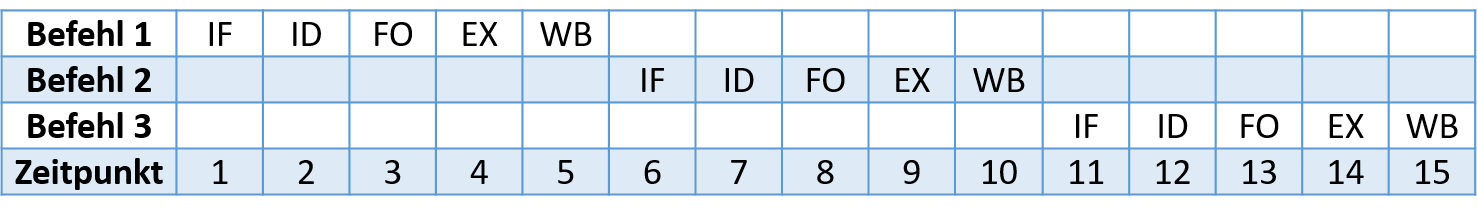
\includegraphics[width=11cm]{Abbildungen/Befehlszylus_ohne_Pipelining.png}
							\caption{Grafische Darstellung der Abarbeitung von drei Befehlen nach dem Schema des Befehlszyklus.}
							\label{fig:BefehlszylusOhnePipelining}
						\end{figure}
				\end{description}
			
				Für eine geraume Zeit in der Geschichte der Rechner war die sequentielle Abarbeitung auch die einzig Mögliche. Bei der Modellierung von Abläufen der Realität, die aus parallelen Vorgängen bestehen, führt die Sequentialisierung zu einer künstlichen Einschränkung, da parallel ablaufende Vorgänge in einem hochwertigen Modell auch parallel ablaufen müssen.
				Um eine bessere Modellierung von parallelen Vorgängen zu ermöglichen, musste folglich ein neues Programmierparadigma definiert werden, welches die Parallelität berücksichtigt. Selbiges ist heute unter dem Namen \textit{Paradigma der Parallelen Programmierung} oder auch \textit{Paralleles Programmierparadigma} bekannt und wird oft eingesetzt. Dieses Paradigma erlaubt es, Parallelverarbeitung auf Ebene der Informatik zu realisieren. Wie und mit welchen Konzepten dies geschieht bzw. geschehen kann, soll im Verlauf dieser Arbeit klar werden.
				
	\section{Gründe für das parallele Programmierparadigma}
				
		Neben der besseren Modellierung von parallelen Vorgängen bietet die Parallelisierung noch einige weitere Vorteile. Schon seit einigen Jahren wird die parallele Programmierung im Bereich des Hochleistungs-Rechnens verwendet. Genauere Simulationen oder auch die Simulationen von komplexeren Problemen benötigen immer mehr Rechenleistung und auch Speicherplatz. Ein oft genanntes Beispiel sind in diesem Zusammenhang die Wetter-Simulationen, welche auf komplizierten mathematischen Modellen basieren. Das Vorhersagen der zukünftigen Entwicklung in der Atmosphäre ist nur durch die Verwendung eines Modells und einer daraus resultierenden Simulation möglich.
		Die Schwierigkeit bei Computer-Simulationen liegt allerdings darin, dass sie meist einen großen Rechenaufwand nach sich ziehen. Ein nicht leistungsfähiger Rechner kann die Simulation selbst oder auch die Genauigkeit des resultierenden Ergebnisses erheblich einschränken. Aus diesem Grund werden Parallelrechner\footnote{Ein Parallelrechner ist ein Rechner, der über mehrere Ausführungseinheiten (z.B. Kerne oder Prozessoren) verfügt und somit echte Parallelverarbeitung unterstützt.} oft im Zusammenhang mit Computersimulationen verwendet. Um solche Rechner ausnutzen zu können, muss die durchzuführende Berechnung in mehrere, kleinere Teile zerlegt werden, welche dann den einzelnen, parallelen Abarbeitungseinheiten zugeordnet werden können. Diese einzelnen Berechnungen sollten unabhängig voneinander ablaufen, und auch der Algorithmus, der angewendet wird, muss in parallel ausführbare Einheiten zerlegbar sein. Um eine parallele Ausführung zu ermöglichen, muss der Algorithmus allerdings in einer Programmiersprache verfasst werden, welche entweder die Parallelisierung direkt, durch Hinzunahme von externen Bibliotheken oder auch durch spezielle Compiler-Direktiven unterstützt, welche zu einer gewöhnlichen Programmiersprache wie beispielsweise C oder Java hinzugefügt werden. \cite{ParaProgRauber}\\
		
		\subsection{Möglichkeiten der Leistungserhöhung}
			\label{MoeglichkeitenLeistungserhoehung}
		
			Eine erhöhte Rechenleistung kann allerdings nicht nur durch Parallelisierung erreicht werden kann. Da die CPU, wie bereits erwähnt, Befehle im einfachsten Fall nur sequentiell abarbeiten kann, eröffnen sich intuitiv zwei Möglichkeiten der Leistungssteigerung:
		
			\begin{enumerate}
				\item Die erste Variante der Erhöhung der Performance besteht in der Beschleunigung der Abarbeitungszeit, die der Prozessor für einen Befehl benötigt. Dieser Lösungsansatz wirkt zunächst passend, da die Prozessoren immer kleiner und billiger werden. Doch diese Entwicklung zu immer kleineren, leistungsfähigeren CPUs ist gewissen physikalische Begrenzungen, wie beispielsweise der Lichtgeschwindigkeit als natürliche obere Grenze der Signalübertragungsgeschwindigkeit, unterworfen. Das Erreichen von Fortschritten bei der Erhöhung der Einprozessorleistung wird folglich immer schwieriger. \cite{GrundlagenParallelisierung}
				\item Angesichts des obigen Problems rücken die Fortschritte in der Netzwerktechnik in den Vordergrund. Die Verbindungen zwischen Rechnern werden immer besser, die Geschwindigkeiten höher und die Bandbreiten größer. Somit wird es in Zukunft einfacher, mehrere Prozessoren miteinander zu verbinden, sodass sie parallel an einem gemeinsamen Problem arbeiten, als die Leistung der einzelnen Komponenten zu erhöhen. \cite{GrundlagenParallelisierung} Solche sogenannte Parallelrechner sind folglich die Zukunft des Hochleistungsrechnens.
			\end{enumerate}

		\subsection{Mooresches Gesetz}
		
			Einer der Mitbegründer von Intel, Gordon Moore, formulierte im Jahr 1965 das nach ihm benannte Mooresche Gesetz. Dieses besagt, dass sich die Anzahl der Transistoren, welche in einem Prozessor enthalten sind, in etwa alle 18 Monate verdoppelt. Diese Aussage traf Moore in Bezug auf die sich damals schnell entwickelnde Halbleiter-Industrie. Zehn Jahre später, im Jahr 1975, relativierte er die von ihm formulierte Regel, indem er die Verdopplung der Anzahl der Transistoren in einem Chip von nun an auf in etwa alle zwei Jahre voraussagte. In diesem Zusammenhang muss allerdings erwähnt werden, dass dieses Gesetz auf Empirie\footnote{Empirie bezeichnet auf Basis von Erfahrung gewonnenes Wissen. \cite{EmpirieDuden}} basiert, und folglich für die Wissenschaft genau genommen keinerlei Bedeutung hat.
			Im Jahr 2003 hielt Moore einen Vortrag über die Zukunft der Halbleiterbranche an der \textit{International Solid-State Cicuits Conference (ISSCC)}, während welchem er sich eingestand, dass das nach ihm benannte Gesetz wohl in den nächsten Jahren seine Gültigkeit verlieren würde. \cite{EndeHardwareMiniaturisierung}\\
			Schenkt man Moore und den Gesetzen der Physik Glauben, so wird die zweite der unter Kapitel  \ref{MoeglichkeitenLeistungserhoehung} genannten Möglichkeit die Zukunft der Informatik bestimmen.
			Die Abbildung \ref{fig:MoorschesGesetz} verdeutlicht nochmals den Zusammenhang zwischen der historischen Entwicklung der Anzahl der Transistoren auf einem Prozessor und dem Mooreschen Gesetz. Dabei sei erwähnt, dass die Skalierung der y-Achse dieses Graphes keineswegs linear ist, sondern logarithmisch erfolgt.
		
			\begin{figure}
				\centering	
				
\includegraphics[width=11cm]{Abbildungen/Moorsches_Gesetz.png}
				\caption{Zusammenhang zwischen der Anzahl der Transistoren in einem Prozessor und dem Mooreschen Gesetz.}
				\label{fig:MoorschesGesetz}
			\end{figure}
		
		\subsection{Trends im Hochleistungsrechnen}
		
			Auch im Bereich des Hochleistungsrechnens werden zunehmend immer mehr Prozessoren verbunden, anstatt wenige leistungsstarke CPUs zu verwenden. Die großen Rechenzentren, wie beispielsweise das Leibniz-Rechenzentrum der Bayrischen Akademie der Wissenschaften (LRZ), verwenden sogenannte Super-Computer, welche aus tausenden von Prozessoren bestehen. Das LRZ ist beispielsweise im Besitz eines Rechners mit dem Namen \textit{SuperMUC}, welcher sich in der Nähe der deutschen Großstadt München befindet. Dieser besteht aus mehr als 241.000 Prozessor-Kernen und erreicht eine Spitzenleistung von mehr als 6,8 Petaflop/s, also mehr als $6,8\cdot10^{15}$ Floating Point Operations Per Second (Gleitkommazahl-Operationen pro Sekunde). Damit ist selbiger einer der aktuell schnellsten Super-Computer. \cite{LRZ}\\
			Somit wird klar, dass das parallele Programmierparadigma in Zukunft wohl noch an Bedeutung gewinnen wird und sich eine Auseinandersetzung mit diesem mittlerweile breitgefächerten Gebiet der Informatik lohnt.
	
	\cleardoublepage
	
	% Abschlussarbeit am Ende der Oberschule
% Facharbeit zum parallelen Programmierparadigma
% Thomas Mittermair
% Oberschulzentrum J. Ph. Fallmerayer Brixen

\chapter{Theoretische Grundbegriffe und Konzepte}

	\section{Grundprinzipien der Parallelisierung}
	
		Bei der Parallelisierung, also der Aufteilung eines Vorgangs in verschiedene, meist voneinander unabhängige Abarbeitungsstränge, existieren einige Grundprinzipien, die beachtet werden müssen und aus diesem Grund im Folgenden näher erläutert werden.	
	
		\subsection{Teile und herrsche (divide and conquer, divide et impera)}
			\label{TeileUndHerrsche}
	
			In der Informatik wird man oft mit Problemen konfrontiert, die als Ganzes betrachtet zunächst nur schwer bewältigbar erscheinen. Aus diesem Grund wurde eine Strategie mit dem Namen \textit{teile und herrsche}, auch \textit{divide and conquer} oder \textit{divide et impera} genannt, entwickelt. Selbige ist für viele Bereiche der Informatik unabdingbar. Dabei wird ein Problem so lange in kleinere Teilprobleme zerlegt, bis sich die entstehenden Teilprobleme einfach lösen lassen. Diese Teillösungen müssen im Anschluss noch zu einer Gesamtlösung kombiniert werden. Diese Vorgehensweise erleichtert oft das Lösen komplexer Probleme, aber auch einfache Sachverhalte können durch die Anwendung dieser Strategie meist eleganter und schneller gelöst werden. \cite{TeileUndHerrsche}\\
			Beispielweise funktioniert der Sortier-Algorithmus \textit{Mergesort} nach diesem Prinzip. Das zu lösende Problem besteht in der Sortierung einer ungeordneten Liste von Einträgen gemäß ihres Schlüssels. Dabei wird die Liste rekursiv in kleinere Teillisten aufgeteilt, bis nur noch Listen übrig bleiben, die aus einem Element bestehen. Listen mit nur einem Element gelten als sortiert. Nun müssen diese Teillösungen noch zu einer Gesamtlösung kombiniert werden. Dabei werden die entstandenen Teillisten wieder zu größeren, aber sortierten Listen zusammengefügt, bis nur noch eine Liste übrig bleibt. Die Liste gilt dann als sortiert. \cite{EinfacheSortierverfahren}\\
			Somit wird klar, dass auch die parallele Programmierung nach dem Prinzip \textit{teile und herrsche} arbeitet. Ein Problem wird hierbei in verschiedenen Teilprobleme aufgeteilt, welche dann parallel abgearbeitet werden können. Dabei muss allerdings beachtet werden, ob Parallelverarbeitung möglich ist, denn nicht jedes Problem ist parallelisierbar. Wenn beispielsweise eine Aufgabe aus Teilaufgaben besteht, die jeweils alle vom Ergebnis der vorhergehenden Teilaufgabe abhängen, so ist durch die Parallelisierung keine Leistungssteigerung möglich. In diesem Fall würden die eigentlich für parallele Arbeit ausgelegten Komponenten nacheinander am Problem arbeiten, was dem Prinzip der Leistungssteigerung widerspricht.

		\subsection{Fork-Join-Modell}
			\label{ForkJoinModell}
			
			Das Fork-Join-Modell ist ein grundlegendes Prinzip im Bereich der Parallelisierung.
			Das englische Verb \textit{to fork} kann dabei mit \textit{gabeln} oder auch \textit{aufspalten} übersetzt werden, das englische Verb \textit{to join} hingegen mit \textit{verbinden} oder auch \textit{zusammenströmen}. Verwendet man dieses Konzept, so existiert in einem Programm zunächst ein Abarbeitungsstrang, der sequentiell Befehle abarbeitet. Kommt das auszuführende Programm zum Punkt, an welchem eine Parallelverarbeitung möglich wird, erstellt dieser Haupt-Abarbeitungsstrang $n$ Kind-Abarbeitungsstränge, welche dann parallel an einem Problem arbeiten. Diese Gabelung des sequentiellen Haupt-Abarbeitungsstranges in mehrere Kind-Abarbeitungsstränge entspricht dem \textit{Fork}. Während die Kind-Abarbeitungsstränge am Problem arbeiten, kann der Haupt-Abarbeitungsstrang, welcher in diesem Zusammenhang auch Eltern- oder Vater-Abarbeitungsstrang genannt wird, entweder auch an der Lösung des Problems mitarbeiten oder auch andere Aufgaben erledigen und muss dann auf die Terminierung der Kind-Abarbeitungsstränge warten. Das Zusammenströmen des Haupt-Abarbeitungsstranges mit den $n$ Kind-Abarbeitungssträngen entspricht dem \textit{Join}, da aus mehreren parallelen Abarbeitungssträngen wieder ein einziger, sequentieller Abarbeitungsstrang wird.\\
			Das Fork-Join-Modell weist den Vorteil auf, dass es eine einfache Erstellung parallel arbeitender Programme ermöglicht\cite{ParaProgRauber}. Aus der Beschreibung dieses Modells lässt sich leicht erkennen, dass das Fork-Join-Modell auf dem Prinzip des unter Punkt \ref{TeileUndHerrsche} erwähnten Prinzips \textit{teile und herrsche} aufbaut.

		\subsection{Lastenverteilung (load balancing)}
		
			Die konsequente Anwendung des unter Punkt \ref{ForkJoinModell} genannten \textit{Fork-Join-Modells} führt zu einer grundlegenden Frage, welcher parallele Handlungsstrang wie viel Arbeit leisten soll und wie die gesamte Arbeit (Last) aufgeteilt werden soll.\\
			Das Hauptziel der Zuweisung der Arbeit an die jeweiligen parallelen Handlungsstränge sollte sein, dass eine hochwertige \textit{Lastenverteilung}, auch \textit{load balancing} genannt, daraus resultiert, das bedeutet, jeder parallele Handlungsstrang sollte, sofern möglich, die gleiche Menge an Berechnung durchführen müssen. \cite{ParaProgRauber}
			Der Grund, warum jeder parallele Handlungsstrang gleich viel Last tragen, also gleich viel Arbeit verrichten sollte, liegt in der Natur des Fork-Join-Modells. Da der Haupt-Abarbeitungsstrang auf die Terminierung \textit{aller} Kind-Abarbeitungsstränge warten muss, ist die parallele Lösung des Problems nur performant, falls alle parallelen Abarbeitungsstränge annähernd gleich viel Zeit für die Abarbeitung benötigen. Das folgende Sprichwort beschreibt diesen Sachverhalt angemessen:
			
				\begin{quote}
					 \textit{Eine Kette ist nur so stark wie ihr schwächstes Glied. \cite{SprichwortKette}}
				\end{quote}
				
			Überträgt man das obige Sprichwort auf die Parallelisierung, so wird aus der Stärke der Kette die Ausführungsgeschwindigkeit des parallelen Teils des Programmes und aus den einzelnen Gliedern der Kette werden die einzelnen, parallelen Abarbeitungsstränge im Programm.
			Das Ziel der Lastenverteilung ist es folglich, die Last so auf die parallelen Abarbeitungsstränge aufzuteilen, dass die geringste Gesamtausführungszeit des Programms daraus resultiert. Das gleichmäßige Aufteilen der Arbeit ist somit das Bestreben dieses grundlegenden Konzepts der parallelen Programmierung.			
			
		\subsection{Parallelität und Nebenläufigkeit}
			
			Im Bereich der Parallelisierung stößt man des Öfteren auf zwei Begriffe, nämlich dem Begriff der \textit{Nebenläufigkeit} und dem der \textit{Parallelität}, welche im Folgenden näher erläutert werden.	
			
			\begin{description}
				\item[Nebenläufigkeit]
				  Zwei Vorgänge nennt man \textit{nebenläufig}, wenn sie vollkommen voneinander unabhängig abgearbeitet werden können. Existieren zwei nebenläufige Vorgänge A und B, so spielt es keine Rolle, ob zuerst Vorgang A und dann Vorgang B abgearbeitet wird oder umgekehrt, oder ob sie sogar gleichzeitig, also parallel, erledigt werden.\\
				  Anweisungen, welche nebenläufig sind, können also parallel und auch auf verschiedenen Prozessoren ausgeführt werden. Werden sie auf einem Prozessor ausgeführt, so kann der Prozessor beliebig zwischen der Abarbeitung des Vorganges A und B hin und her wechseln und die Abarbeitungsreihenfolge ist somit nicht von Bedeutung.
			  \item[Parallelität]
				  Zwei Vorgänge nennt man \textit{parallel}, wenn sie gleichzeitig und unabhängig voneinander abgearbeitet werden können. Die Anweisungen zweier Vorgänge werden also parallel bearbeitet, wenn die Anweisungen unabhängig voneinander zur selben Zeit erledigt werden. Eine parallele Bearbeitung ist somit immer auch nebenläufig.
			\end{description}
			
			Somit wird klar, dass \textit{Nebenläufigkeit} ein allgemeinerer Begriff als \textit{Parallelität} ist. \cite{NebenlaeufigeProg}

	\section{Implementierungsmöglichkeiten der Parallelisierung}
	
		Die Parallelisierung kann auf verschiedensten Arten realisiert werden. Im Allgemeinen lassen sich allerdings zwei Ebenen unterscheiden: Die Software- und Hardwareebene.
				
		\subsection{Implementierungsmöglichkeiten der Parallelisierung auf Softwareebene}

			Softwaretechnisch existieren zwei grundlegende Arten, um Parallelisierung zu implementieren: \textit{Prozesse} und \textit{Threads}.
			Dabei spielt das Betriebssystem eines Rechners eine zentrale Rolle, da es dem Software-Entwickler die nötigen Instrumente zur Verfügung stellt, um solche Prozesse und Threads zu erstellen.\\
			Heutige Rechner sind dazu in der Lage, mehrere Aktionen gleichzeitig zu erledigen. Ein Computer liest beispielsweise Daten von der Festplatte, gibt Inhalte auf dem Bildschirm aus und gleichzeitig laufen auch noch einige Anwendungsprogramme des jeweiligen Benutzers.\\
			Zunächst muss klargestellt werden, dass ein gewöhnlicher Rechner nicht so viele CPUs enthält wie Aufgaben abzuarbeiten sind. Somit ist der Prozessor dazu gezwungen, zwischen der Abarbeitung der einzelnen Programme zu wechseln. Zu jedem beliebigen Zeitpunkt wird also stets nur ein Programm gleichzeitig auf einer CPU bearbeitet. Durch das schnelle Wechseln zwischen den Programmen wird beim Benutzer die Illusion von Parallelität geweckt. Um eine klar Abgrenzung zwischen dieser vorgetäuschten Parallelität und der echten Hardware-Parallelität zu schaffen, spricht man von \textit{Quasiparallelität}. \cite{ModerneBetriebssysteme}
			
			\subsubsection{Das Prozess-Modell}
				\label{ProzessModell}
			
				Im Rahmen dieses Modells ist die Gesamtheit aller auszuführenden Programme als eine Menge von sequentiellen Prozessen organisiert. Solche sequentielle Prozesse werden oft auch nur Prozesse genannt.
				Ein Prozess ist dabei ein Programm in Ausführung, wobei zentrale Aufgaben wie beispielsweise die Zuteilung der Ressourcen (z.B. der CPU) dem Betriebssystem überlassen werden.\\
				Für jeden Prozess wird der Eindruck erweckt, dass er selbst eine CPU zur Verfügung habe und jeder Prozess somit tatsächlich parallel ablaufen würde. In der Realität ist dies nur selten der Fall, meist handelt es sich bei dieser CPU nur um eine virtuelle CPU und die reale CPU schaltet zwischen den Prozessen hin und her. Folglich kommt meist Quasiparallelität zum Einsatz. Die kleinen Einheiten an Rechenzeit, welche die einzelnen Prozesse erhalten, werden als Zeitscheiben bezeichnet.\\
				Jeder Prozess besitzt eine individuelle Aufgabe und auch eine eigene Ablaufsteuerung, also einen eigenen Befehlszähler, welcher angibt, welcher Befehl des Programmes als Nächster abgearbeitet werden muss.\\
				Somit ist die grundlegende Idee, dass jeder Prozess eine Aktivität beliebiger Art ist. Er hat ein Programm, welches festlegt, welche und wie die Aufgabe abgearbeitet werden muss, Eingabedaten, Ausgabedaten und einen Zustand.
				Das Programm beschreibt im Unterschied zum Prozess also nur das Verfahren, also den Algorithmus, mit welchem eine Aufgabe gelöst werden soll. Die Aktivität des Lösens dieser Aufgabe unter der Verwendung des Programmes als Anleitung wird als Prozess bezeichnet.
				Der Ansatz des Erstellens von mehreren Prozessen auf einem Rechner, welche dann (quasi-)parallel arbeiten, wird auch als \textbf{Multiprocessing} bezeichnet. \cite{ModerneBetriebssysteme}
				
				\begin{description}
					\item[Prozesszustand]
						\label{Prozesszustand}
						
						Obwohl jeder Prozess eine unabhängige Einheit darstellt, kommt es oft zu Situationen, in welchen Prozesse sich austauschen müssen, um Aufgaben korrekt zu erledigen.\\
						Führt ein Prozess A beispielsweise eine Berechnung durch, die zu einem Ergebnis führt, welches von einem weiteren Prozess B benötigt wird, damit selbiger eine Aufgabe abarbeiten kann, so muss der Prozess B so lange blockiert werden, bis die Ergebnisse von Prozess A zur Verarbeitung bereitstehen.\\
						Des Weiteren ist es möglich, dass die Zeitscheibe eines Prozesses, der gerade eine Aufgabe mit Hilfe der CPU erledigt, abläuft. Somit wäre er zwar rechenbereit, kann allerdings keine Berechnungen durchführen, da er im Moment nicht über eine Ausführungseinheit verfügt.\\
						Die genannten Situationen lassen sich mit Hilfe von sogenannten \textit{Prozesszuständen} lösen. Ein Prozess kann im Allgemeinen fünf grundlegende Zustände annehmen, welche im Folgenden erläutert werden.
						
						\begin{enumerate}
							\item \textbf{Erstellt-Zustand}: Der Prozess wurde erstellt und ist bereit, die ihm zugewiesene Aufgabe abzuarbeiten.
							\item \textbf{Rechnender Zustand, Aktiv-Zustand}: Der Prozess führt gerade Berechnungen unter Verwendung der CPU durch, ihm wurde folglich eine Zeitscheibe zugewiesen.
							\item \textbf{Rechenbereiter Zustand, Bereit-Zustand}: Der Prozess wäre zum Rechnen in der Lage, verfügt im Moment aber über keine CPU.
							\item \textbf{Blockiert-Zustand}: Der Prozess ist nicht zum Rechnen imstande, bis ein bestimmtes Ereignis eintritt, also bis beispielsweise Daten zur Verfügung stehen. In diesem Zustand könnte der Prozess auch, falls er die CPU erhalten würde, keine Berechnungen durchführen. Das Zuteilen von Ressourcen an einen blockierten Prozess ist folglich nicht sinnvoll.
							\item \textbf{Beendet-Zustand}: Der Prozess hat seine Aufgabe vollfüllt oder wurde auf Grund eines Problems beendet.
						\end{enumerate}
					
						Die Abbildung \ref{fig:Prozesszustaende} soll die Prozesszustände nochmals verdeutlichen. Dabei ist der Übergang vom aktiven in den blockierten Zustand der einzige Zustandswechsel, den der Prozess selbst auslösen kann. Alle anderen werden vom Betriebssystem veranlasst. \cite{ModerneBetriebssysteme}
						
						\begin{figure}
							\centering	
							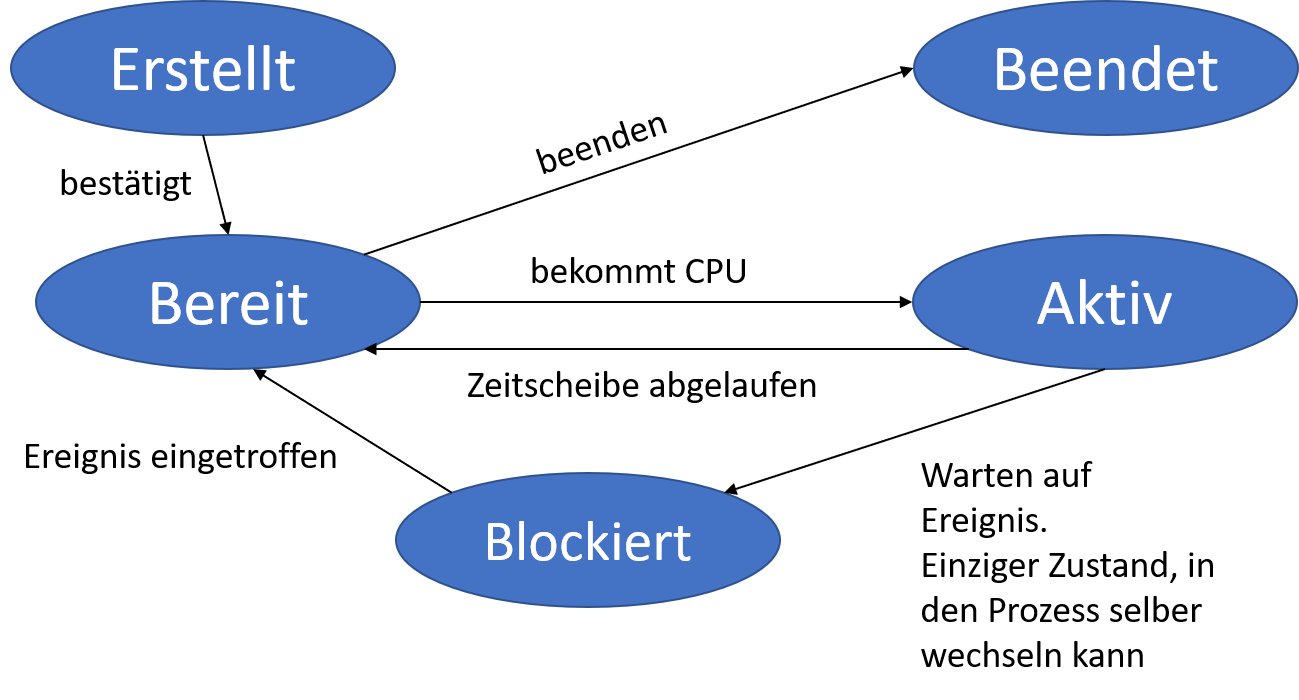
\includegraphics[width=11cm]{Abbildungen/Prozesszustaende.png}
							\caption{Grafische Darstellung der fünf grundlegenden Prozesszustände.}
							\label{fig:Prozesszustaende}
						\end{figure}
		
					\item[Prozesshierarchie]
						\label{Prozesshierarchie}
						
						Ein Prozess ist dazu in der Lage, weitere Prozesse zu starten. Startet ein Prozess A einen neuen mit dem Namen B, so bildet sich zwischen den beiden Prozessen eine Hierarchie: Der Prozess A ist der Vaterprozess, während der Prozess B der Kindprozess ist. Jeder Prozess hat dabei genau einen Vaterprozess, allerdings beliebig viele Kindprozesse.\\
						Aus dem obigen Konzept wird nicht klar, wie ein Rechner-System startet, da zu Beginn ein Prozess gestartet werden muss, welcher der erste Prozess im System ist und somit keine Vaterprozess haben kann.\\
						Das Betriebssystem UNIX löst diese Problematik mittels eines eigenen Prozesses mit dem Namen \textit{init}, welcher im Boot-Abbild des System gespeichert ist. Beim Systemstart wird dieses Boot-Image gelesen und der Prozess \textit{init} erzeugt. Dieser Prozess kann dann wiederum Kindprozesse starten, welche dann auch Kindprozesse starten können usw. Somit initialisiert sich das Betriebssystem beim Start selbst. Daraus ergibt sich eine die gesamte System umfassende Prozess-Hierarchie, welche baumartig aufgebaut ist und wobei die Wurzel des Baumes der Prozess \textit{init} ist.\\
						Unter Windows gibt es kein Konzept der Prozesshierarchie, alle Prozesse sind hier gleichwertig. \cite{ModerneBetriebssysteme}
		
					\item[Eigenschaften eines Prozesses]
						
						Ein Prozess hat einige wichtige Eigenschaften. Auf die wichtigsten Merkmale soll im Folgenden eingegangen werden.
						
						\begin{itemize}
							\item Jeder Prozess besitzt eine eigene Prozessumgebung. Das bedeutet er besitzt eine eigene Aufgabe, einen eigenen Speicher-Adressraum und auch einen eigenen Ausführungsfaden. Damit geht einher, dass jeder Prozess seine Aufgabe individuell abarbeiten kann.
							\item Jeder Prozess kann andere Prozesse erzeugen, welche dann Kindprozesse genannt werden.
							\item Jeder Prozess kann mit anderen Prozessen kommunizieren. Man spricht hier von IPC (Inter-Prozess-Kommunikation), wobei das Betriebssystem Kommunikations-Methoden anbietet.
							\item Jedem Prozess wird ein sogenannter \textit{Adressraum} zugeordnet. Dieser besteht aus einer Liste von Speicherstellen, auf die der Prozess Lese- und Schreibzugriffe ausführen darf.
							\item Prozesse können voneinander abhängen. Dies ist beispielsweise der Fall, wenn ein Prozess erst arbeiten kann, sobald er das Ergebnis eines anderen Prozesses erhalten hat. In diesem Fall ist Prozess-Synchronisation nötig, auf welche in Kapitel \ref{ProzessSynchronisation} eingegangen wird. \cite{ModerneBetriebssysteme}
						\end{itemize}
						
					\item[Scheduling von Prozessen]
						\label{ProzessScheduling}
						
						Auf den modernen Betriebssystemen ist die Existenz mehrerer Prozesse zur gleichen Zeit keine Seltenheit, sondern die Regel. Falls weniger physikalische CPUs vorhanden sind als parallel ablaufende Prozesse, so müssen die CPUs zwischen verschiedenen Prozessen wechseln. Des Weiteren muss es eine Instanz geben, welche entscheidet, welcher Prozess als Nächster eine Zeitscheibe zugewiesen bekommt und auch die Länge der Zeitscheibe muss festgelegt werden. Der Teil des Betriebssystems, welche für diese Aufgaben zuständig ist, wird \textit{Scheduler} (englisch für \textit{Zeitplaner}) genannt.\\
						Der Scheduler teilt den Prozessen folglich die CPU zu. Er weiß allerdings nie genau, welche Ressourcen in Zukunft angefragt werden und welche zur Verfügung stehen werden. Der Scheduling-Algorithmus muss daher schätzen und dynamisch auf Änderungen reagieren. Es gestaltet sich folglich schwierig, ein geeignetes Verfahren zu finden, um den nächsten Prozess, der eine Zeitscheibe erhalten soll, auszuwählen. Aus diesem Grund haben sich verschiedene Strategien im Laufe der Geschichte entwickelt. Im Folgenden werden exemplarische einige Strategien erklärt. Dabei wird eine Unterteilung in Scheduling auf Stapelverarbeitungs-Systemen und interaktiven Systemen gemacht.
						
						\begin{description}
							\item[Scheduling auf Stapelverarbeitungs-Systemen]~\par	% ~\par führt zu einem Zeilenumbruch.

								\begin{itemize}
									\item
										\textbf{First Come - First Serve (FCFS)}: Den Prozessen wird die CPU in der Reihenfolge zugewiesen, in der sie sie anfordern. Somit entsteht eine Warteschlange von rechenbereiten Prozessen. Sobald ein Prozess in den blockierten Zustand übergeht, kommt der nächste Prozess an die Reihe und der blockierte Prozess reiht sich nach dem Verlassen des blockierten Zustandes wieder in die Warteschlange ein. Ein Vorteil dieses Verfahrens ist, dass die CPU optimal ausgenutzt wird. Allerdings kann die Abarbeitung eines aufwendigen Prozesses die Ausführungs kleiner Prozesse verzögern oder sogar verhindern.
									\item
										\textbf{Shortest Job First (SJF)}: Bei diesem Algorithmus wird davon ausgegangen, dass die Abarbeitungszeiten, also die Zeiten, wie lange die Prozesse zur Abarbeitung benötigen, im Vornherein bekannt sind. Dies ist beispielsweise anhand von Erfahrungswerten möglich. Der Prozess, der die kleinste Abarbeitungszeit besitzt, bekommt in diesem Fall die CPU. Dieses Verfahren funktioniert, falls die Abarbeitungszeiten durch Erfahrungen bekannt sind. Allerdings kann es passieren, dass sich die Bearbeitung aufwendiger Prozesses verzögert oder im schlimmsten Fall diese Prozesse die CPU sogar nie erhalten.
								\end{itemize}
							
							\item[Scheduling auf interaktiven Systemen]~\par	% ~\par führt zu einem Zeilenumbruch.
							
								\begin{itemize}
									\item
										\textbf{Round-Robin-Scheduling (Zeitscheiben-Verfahren)}: Dies ist eine der am meisten verwendeten Scheduling-Strategien. Jedem Prozess wird dabei eine Zeitscheibe zugewiesen, für welche er die CPU bekommt. Nach Ablauf der Zeitscheibe wird dem Prozess der Prozessor entrissen und an den nächsten Prozess gegeben. Falls ein Prozess vor Ablauf der Zeitscheibe blockiert oder beendet wird, so endet seine Zeitscheibe vorzeitig und der nächste Prozess kann mit seinen Berechnungen beginnen. Somit ergibt sich auch hier eine Warteschlange, wobei jeder Prozess der Reihe nach die CPU bekommt und sich nach der Bearbeitung durch die CPU entweder beendet, blockiert wird oder sich wieder am Ende der Warteschlange einreiht. Im einfachsten Fall des Round-Robin-Verfahrens wird davon ausgegangen, dass alle Prozesse gleich wichtig sind und dadurch alle Prozesse gleich große Zeitscheiben zugewiesen bekommen. Eine Abwandlung dieses Verfahrens ist das \textit{Weighted Round-Robin-Scheduling}. Bei diesem Algorithmus können die Zeitscheiben je nach Prozess unterschiedlich lang sein. Ein Nachteil dieses Verfahrens ist allerdings, dass dringende Prozesse nicht vorgezogen werden können.
									\item
										\textbf{Prioritätenbasiertes Scheduling}: Bei Verwendung des Round-Robin-Scheduling ist jeder Prozess gleich wichtig. Denkt man allerdings an die Realität, so gibt es des Öfteren Aktivitäten, die wichtiger sind als andere. Ein Prozess, der im Hintergrund E-Mails verschickt, sollte von geringerer Wichtigkeit sein als ein Prozess, der für die Darstellung von Videos in Echtzeit zuständig ist. Aus diesem Grund stellt das prioritätenbasierte Scheduling eine Weiterentwicklung des Round-Robin-Schedulings dar. Jeder Prozess bekommt bei diesem Verfahren zusätzlich eine Priorität zugewiesen und der Prozess mit der aktuell höchsten Priorität erhält die CPU. Jedem Prozess muss in diesem Zusammenhang auch noch eine maximale Zeitscheiben-Dauer zugewiesen werden, um zu verhindern, dass der Prozess mit der größten Priorität ewig läuft. Nach dem Ablauf dieses Maximums an CPU-Zeit muss dann ein Prozesswechsel passieren, wobei der Prozess mit der nächst-größten Priorität an die Reihe kommt. Bei mehreren Prozessen mit gleich großer Priorität kann FCFS angewendet werden. \cite{ModerneBetriebssysteme}
								\end{itemize}
						\end{description}
				\end{description}
			
			\subsubsection{Das Thread-Modell}

				Im Rahmen des bereits bekannten Prozess-Modells, welches unter Kapitel \ref{ProzessModell} erläutert wurde, hat jeder sequentielle Prozess einen eigenen Adressraum und auch einen eigenen Ausführungsfaden, wobei die einzelnen Prozesse auf einem System parallel zueinander ablaufen.\\
				Es hat sich in der Vergangenheit allerdings herausgestellt, dass es oft von Vorteil ist, mehrere Ausführungsfäden parallel bzw. quasiparallel zueinander innerhalb desselben Adressraums ablaufen zu lassen. Die einzelnen Ausführungsfäden verhalten sich dann ähnlich wie getrennte Prozesse, wobei der größte Unterschied der gemeinsame Adressraum darstellt.\\
				Die zwei Grundkonzepte von Prozessen sind die \textit{Bündelung der Ressourcen} und die \textit{Ausführung}.
				
				\begin{itemize}
					\item
						Ein Prozess lässt sich als eine Gruppierung von Ressourcen unterschiedlichster Art betrachten. Dazu zählen Quelltext, Programm-Daten, geöffnete Dateien, und vieles mehr. All diese Ressourcen sind im Adressraum des Prozesses und somit im Hauptspeicher des Rechners abgelegt.
					\item
						Das zweite wichtige Konzept ist die Ausführung. Ein Prozess besitzt im einfachsten Fall genau einen \textit{Ausführungsfaden}, auf Englisch auch \textit{Thread}\footnote{Der englische Begriff \textit{Thread} kann mit dem deutschen Wort \textit{Faden} übersetzt werden.} genannt. Eigentlich besitzt nicht der Prozess selbst, sondern der ihm innewohnende Thread den Befehlszähler, welcher angibt, welcher Befehl als Nächster abgearbeitet werden soll.
				\end{itemize}
			
				Ein Thread ist zwar stets von seinem Prozess existenzabhängig, jedoch sind Prozess und Thread zwei getrennte Konzepte. Das Konzept von Threads erweitert das Prozess-Modell, da ein Prozess nicht nur einen Thread enthalten kann, sondern beliebig viele. Somit können mehrere voneinander unabhängige Ausführungsfäden innerhalb einer Prozessumgebung mit einem gemeinsamen Adressraum realisiert werden. Durch die Einführung von Threads wird ein Prozess auf das Prinzip der Zusammenfassung von Ressourcen und des Bereitstellens einer Umgebung für seine Threads reduziert. Das zweite Grundkonzept des Prozess-Modells, nämlich die Ausführung, geht bei dieser Art der Betrachtung vollständig auf das Thread-Modell über.\\
				Mehrere Threads parallel innerhalb eines Prozesses laufen zu lassen verhält sich ähnlich wie mehrere Prozesse parallel auf einem Rechner laufen zu lassen. Im ersten Fall teilen sich die Threads die Ressourcen des Prozesses (Adressraum, geöffnete Dateien, ...), im zweiten Fall teilen sich die Prozesse die Ressourcen des Rechners (Festplatte, Drucker, ...). Threads und Prozesse befinden sich allerdings auf verschiedenen Ebenen.\\
				Threads werden in der Fachliteratur auf Grund ihrer Ähnlichkeit zu Prozessen manchmal auch als \textit{leichtgewichtige Prozesse} bezeichnet.\\
				Der Ansatz des Erstellens von mehreren Threads innerhalb eines Prozesses wird auch als \textbf{Multithreading} bezeichnet. Läuft auf einem System mit nur einer CPU ein Prozess mit mehreren Threads, so wechseln sich die Threads in der Ausführung ab. Die CPU wechselt ähnlich zu den Prozessen auch hier zwischen den Threads hin und her, sodass wiederum die Illusion von parallel ablaufenden Threads erzeugt wird. \cite{ModerneBetriebssysteme}
				
				\begin{description}
					\item[Eigenschaften von Threads]
					
						Ein Thread hat einige wichtige Eigenschaften, die ihn von einem Prozess unterscheiden. Auf die wichtigsten Merkmale soll im Folgenden eingegangen werden.
						
						\begin{itemize}
							\item
								Alle Threads eines Prozesses teilen sich die Ressourcen des Prozesses und somit auch seinen Adressraum. Damit geht einher, dass alle Threads dieselben globalen Variablen besitzen. Die Threads teilen sich somit auch beispielsweise alle geöffneten Dateien und ähnliche Ressourcen des Prozesses. Dabei kann es zu unvorhergesehenen Problemen, sogenannten \textit{zeitkritischen Abläufen}, kommen. Diese potentiell gefährlichen Situationen lassen sich mittels \textit{Prozess-Synchronisation} entschärfen, auf welche in Kapitel \ref{ProzessSynchronisation} eingegangen wird.
							\item
								Ein Thread kann wie auch jeder Prozess in die unter Punkt \ref{Prozesszustand} beschrieben Zustände geraten. Die fünf Grundzustände lauten auch hier Erstellt-Zustand, Aktiv-Zustand, Bereit-Zustand, Blockiert-Zustand und Beendet-Zustand.
							\item
								Threads dienen der Erstellung mehrerer Ausführungsfäden, welche sich die Ressourcen des Prozesses, zu dem sie gehören, teilen und somit eng und schnell an einer gemeinsamen Aufgabe arbeiten können.
							\item
								Auch zwischen Threads können Hierarchien analog zu Prozessen aufgebaut werden. Dabei sei auf den Punkt \ref{Prozesshierarchie} verwiesen. \cite{ModerneBetriebssysteme}
						\end{itemize}
					
					\item[Fork-Join-Modell bei Threads]
						
						Während Prozesse meist vollkommen unterschiedliche Aufgaben erledigen, arbeiten bei Einsatz von Multithreading die Threads eines Prozesses meist gemeinsam an einem Problem. Hier bietet sich das unter Punkt \ref{ForkJoinModell} erwähnte Fork-Join-Modell an.\\
						Dabei startet ein Prozess zunächst mit einem einzigen Thread, dem Haupt-Abarbeitungsstrang. Dieser Thread verfügt über die Möglichkeit, neue Threads zu erzeugen. Der Haupt-Thread muss dabei den Kind-Threads mitteilen, welche Aufgabe sie lösen müssen. Der Haupt-Thread kann nun entweder selbst auch Berechnungen durchführen oder auch direkt auf die Beendigung seine Kind-Threads warten und das Ergebnis der einzelnen Threads aufsammeln und zu einer Gesamt-Lösung kombinieren. \cite{ModerneBetriebssysteme} \cite{ParaProgRauber}
					
					\item[Verwendung von Threads]
						
						Threads werden immer dann verwendet, wenn innerhalb einer Anwendung mehrere Aufgaben gleichzeitig bewältigt werden müssen, wobei sich diese Aktivitäten gegenseitig blockieren können. Das Aufspalten einer Anwendung in mehrere (quasi-)parallel ablaufende Threads vereinfacht auch die Programmierung, falls es sich um eine Anwendung handelt, die Parallelverarbeitung erlaubt.\\
						Das zuvor genannte Konzept des gemeinsamen Adressraumes ist das zentrale Konzept für die Verwendung von Threads. Threads erweitern somit das Prozess-Modell um die Fähigkeit von (quasi-)parallelen Abarbeitungs-Strängen, die die Daten und Ressourcen des Prozesses gemeinsam nutzen.\\
						Ein weiteres Argument für die Verwendung von Threads ist, dass sie an keine Ressourcen wie z.B. offene Dateien gebunden sind, und somit schneller erstellt und zerstört werden können. In vielen Systemen ist die Erstellung eines Threads 100 Mal schneller als die Erstellung eines Prozesses. \cite{ModerneBetriebssysteme}
						
					\item[Joinable und Detached Threads]
					
						Normalerweise sind Threads \textit{joinable}. Dies bedeutet, dass man vom Vater-Thread aus durch Aufruf einer bestimmten vom Betriebssystem zur Verfügung gestellten Funktion auf die Beendigung des jeweiligen Kind-Threads warten kann. Der diese Funktion aufrufende Vater-Thread wird dabei so lange blockiert, bis der Kind-Thread beendet wurde. Dann kann der Vater-Thread auch eventuelle Rückgabewerte des Kind-Threads einsammeln. Ein joinable Thread \textit{joint} (zu Deutsch \textit{zusammenstörmen}) also zum Vater-Thread zurück, bevor er sich beendet.
						Er wird so lange nicht als beendet betrachtet, bis er mit einem anderen Thread gejoint wird.\\
						Oft kommt es allerdings auch vor, dass ein Kind-Thread nichts zurückgibt und somit kein Bedarf besteht, dass der Vater-Thread auf die Beendigung des Kind-Threads warten müsste. Setzt man bei einem Thread die Eigenschaft von \textit{joinable} auf \textit{detached} (zu Deutsch \textit{losgelöst}), so wird dem System klargemacht, dass man einen Thread erstellt hat, auf dessen Beendigung nicht gewartet werden muss. Somit wird dieser losgelöste Thread beendet, sobald er seine Aufgabe erledigt, wobei kein Join-Vorgang nötigt ist, oder sobald der Prozess, zu welchem er gehört, beendet wird. \cite{ParaProgRauber} \cite{ThreadsRheinwerk}
						
					\item[Scheduling von Threads]
					
						Auf modernen Systemen ist es die Regel, dass mehrere Prozesse parallel ablaufen, welche wiederum jeweils aus mehreren Threads bestehen. Somit liegen zwei verschiedene Ebenen der Parallelität vor, nämlich Prozesse und Threads gleichzeitig. Für das Scheduling in diesem Fall gibt es grundsätzlich zwei verschiedene Ansätze.\\
						Der erste Ansatz ist dem Prozess-Scheduling sehr ähnlich. Der Prozess-Scheduler weist dabei einfach den einzelnen Prozessen die CPU nach einer bestimmten Strategie zu, ohne Rücksicht auf die Threads innerhalb der Prozesse zu nehmen. Somit muss in jedem Prozess nochmals ein Thread-Scheduler existieren, welcher dann den Thread auswählt, der die CPU tatsächlich bekommt, sobald der jeweilige Prozess den Prozessor erhält. Innerhalb einer Zeitscheibe eines Prozesses können somit mehrere Threads bearbeitet werden, da der Thread-Scheduler die Prozess-Zeitscheibe nochmals in kleinere Zeitscheiben unterteilen kann, welche dann wiederum den Threads zugewiesen werden können. Bei diesem Ansatz können sowohl der Prozess-, als auch der Thread-Scheduler Strategien anwenden, welche ähnlich zu den unter Punkt \ref{ProzessScheduling} genannten Strategien sind.
						Der zweite Ansatz besteht darin, dass der Scheduler nicht mehr zwischen Prozessen unterscheidet, sondern nur noch über eine Liste von Threads verfügt, von denen er weiß, dass diese rechenbereit sind. Somit wird die Grenze zwischen den Prozessen aufgehoben und der Fokus liegt auf den Threads, also den Abarbeitungssträngen. Auch bei diesem Ansatz kann der Scheduler Strategien anwenden, welche ähnlich zu den unter Punkt \ref{ProzessScheduling} genannten Strategien sind. \cite{ModerneBetriebssysteme}
				\end{description}
			
		\subsection{Implementierungsmöglichkeiten der Parallelisierung auf Hardwareebene}

			Auf Ebene der Hardware gibt es eine Vielzahl von Möglichkeiten, Parallelisierung zu implementieren. Im Folgenden werden dabei exemplarisch drei Varianten in ihren Grundzügen erläutert.
			
			\subsubsection{Pipelining}
			
				Wie aus Punkt \ref{SequUndParaInformatik} ersichtlich wird, erfolgt die Abarbeitung eines Befehls in einem Prozessor wie an einem Fließband (engl. Pipeline), der Befehl durchläuft also mehrere, in diesem Fall fünf, Stufen. Zunächst wird der Befehl geladen, dann dekodiert, danach werden die Operanden geladen, der Befehl ausgeführt und das Ergebnis schließlich in den Speicher zurückgeschrieben.\\
				Betrachtet man erneut die Abbildung \ref{fig:BefehlszylusOhnePipelining}, so erkennt man, dass die Hardware bei dieser Art der Befehlsausführung nicht effizient ausgenutzt wird. Betrachtet man die fünf Phasen der Befehlsausführung als Stufen einer Pipeline, so kann man die Befehlsausführung auch anders, überlappend, organisieren. Man nutzt also aus, dass die auf einem Prozessor befindlichen Funktionseinheiten bei der Abarbeitung eines Befehls kaum alle gleichzeitig beansprucht werden. Wenn ein Befehl eine Phase abschließt, so muss diese Phase nicht bis zum Abschluss der gesamten Befehlsabarbeitung ungenutzt bleiben, sondern der nächste Befehl könnte direkt diese Phase betreten. Somit wird innerhalb der Pipeline versucht, alle Stufen gleichzeitig für aufeinanderfolgende Befehle zu nutzen und somit die Hardware-Auslastung zu verbessern. Dadurch werden mehrere Befehle gleichzeitig abgearbeitet. Die Pipeline-Verarbeitung kommt in vielen modernen Prozessoren zum Einsatz.\\
				Die Vorteile der Pipeline-Verarbeitung im Gegensatz zur Sequentialität des Befehlszyklus soll nun an Hand eines Beispiels der Abarbeitung von drei Befehlen verdeutlicht werden.
				Die Abbildung \ref{fig:BefehlszylusMitPipelining} soll diesen Vorgang grafisch veranschaulichen. Nimmt man an, dass die Bearbeitung in jeder Phase im Optimalfall einen Taktzyklus benötigt, so dauert die Ausführung dieser drei Befehle ohne Pipelining ganze 15 Taktzyklen, während die Verwendung von Pipeling zu einer Abarbeitungsdauer von 8 Taktzyklen führt. Dies entspricht nahezu einer Halbierung der benötigten Zeit, ohne zusätzliche Hardware ankaufen zu müssen. Des Weiteren wird, sobald die Pipeline-Bearbeitung begonnen hat - zumindest theoretisch, falls keine Verzögerungen eintreten - in jedem Taktzyklus ein Befehl abgeschlossen, während dies bei der sequentiellen Bearbeitung nur alle fünf Taktzyklen passiert. Somit wird klar, dass sich Pipelining durchaus lohnt.\\
				Nicht immer kann eine Pipeline allerdings optimal ausgenutzt werden. Es existieren drei verschiedene Situationen, in denen der nächste Befehl nicht im darauffolgenden Taktzyklus bearbeitet werden kann. Diese Situationen werden \textit{Pipeline Hazards} genannt. Die drei verschiedenen Typen sind:
				
				\begin{itemize}
					\item Strukturkonflikt (\textit{Structural hazard})
					\item Datenkonflikt (\textit{Data hazard})
					\item Steuerkonflikt (\textit{Control hazard}) \cite{AufbauFunktionsweiseMikroprozessoren} \cite{RechnerorganisationUndEntwurf}
				\end{itemize}

				\begin{figure}
					\centering	
					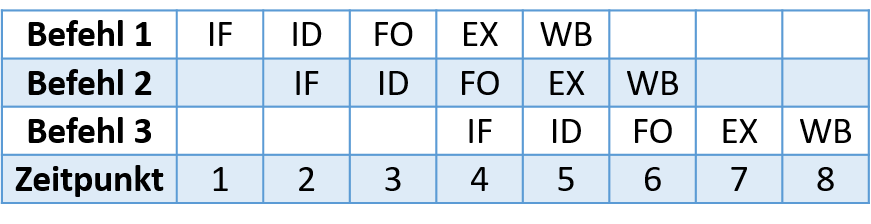
\includegraphics[width=11cm]{Abbildungen/Befehlszylus_mit_Pipelining.png}
					\caption{Grafische Darstellung der Abarbeitung von drei Befehlen nach dem Schema des Befehlszyklus unter Anwendung der Pipelining-Verarbeitung.}
					\label{fig:BefehlszylusMitPipelining}
				\end{figure}
			
			\subsubsection{Vektorrechner}
				\label{Vektorrechner}
				
				Eine weitere Möglichkeit der Realisierung von Parallelem Rechnen sind die sogenannten \textit{Vektorrechner}, auch \textit{Vektorprozessoren} oder \textit{Arrayrechner} genannt.\\
				Das im Namen dieser Technologie enthaltene \textit{Vektor} oder \textit{Array} rührt daher, dass die gleichen Berechnungen gleichzeitig auf einer Menge von Daten ausgeführt werden. Diese Daten sind in diesem Fall meist in Form eines \textit{n}-elementigen Arrays, also eines \textit{n}-dimensionalen Vektors, organisiert.
				Diese Art der Prozessoren sind den gewöhnlichen CPUs, welche die gleiche Operation nacheinander auf den Daten ausführen würden, um ein Vielfaches überlegen, falls es sich bei der zu bewerkstelligenden Aufgabe um eine Operation handelt, die auf viele Daten ausgeführt werden muss. Somit können sich erhebliche Performance-Gewinne erzielen lassen.\\
				Vektorrechner werden vor allem in der Simulationstechnik verwendet, wo viele gleichartige Daten auf gleiche Weise verarbeitet werden müssen. Dies ist beispielsweise in der Geologie und Meteorologie des Öfteren der Fall.
				Allerdings birgt diese Technologie den Nachteil, dass keine Standard-CPUs hier verwendet werden können, da das Vektorrechnen in der Hardware der CPU implementiert sein muss. Aus diesem Grund ergeben sich für Vektorrechner meist erhöhte Kosten im Vergleich zu gewöhnlichen Prozessoren. In der jüngeren Vergangenheit entfernte sich der Trend somit von dieser Art der Parallelrechner und ging zu großen Rechen-Clustern über. Dies sind Verbünde von vielen Standardprozessoren, die über schnelle Leitungen verbunden sind. Dadurch können Kosten eingespart werden, da durch die industrielle Herstellung der Preis von gewöhnlichen CPUs stark gesunken ist.\\
				Da gewöhnliche CPUs nicht mit Vektoren von Daten arbeiten können, werden sie unter Betrachtung der mathematischen Hintergründe auch \textit{Skalarprozessoren} genannt. \cite{VektorrechnerWikipedia}
			
			\subsubsection{Hyper-Threading}
			
				\textit{Hyper-Threading} ist eine Technologie von Intel, die hardwareseitiges Multithreading auf Prozessorebene möglich macht. Dabei wird eine physisch vorhandene CPU in zwei oder mehrere logische Prozessoren aufgeteilt. Die physikalisch vorhandenen Ressourcen werden dabei geteilt, wodurch für die Anwendungen und auch für das Betriebssystem der Eindruck entsteht, dass zwei CPUs vorhanden wären, obwohl dies in Realität nicht der Fall ist. Dahinter steht die Idee, dass ein Prozessor grundsätzlich besser ausgelastet werden kann, indem die Lücken in der Pipeline, welche beispielsweise entstehen, wenn ein Prozess oder Thread auf den Hauptspeicher warten muss, füllt. Das Füllen entspricht in diesem Fall dem Einschieben eines anderen Prozesses oder Threads für die Zeit, in der der andere Prozess blockiert ist. \cite{HyperThreadingIntel} \cite{HyperThreadingWikipedia}

	\section{Prozess-Synchronisation}
		\label{ProzessSynchronisation}
	
		Auch wenn Prozesse an sich als vollkommen voneinander unabhängige Abarbeitungseinheiten betrachtet werden können, besteht doch in vielen Fällen die Notwendigkeit, dass Prozesse untereinander kommunizieren müssen. Diese Art des Austausches von Informationen wird als \textit{Interprozesskommunikation}, kurz \textit{IPC}, bezeichnet.\\
		Dabei müssen allerdings drei wichtige Punkte beachtet werden.
		
		\begin{itemize}
			\item Den Prozessen müssen Möglichkeiten des Austausches von Informationen bereitgestellt werden.
			\item Mehrere kooperierende Prozesse dürfen sich bei kritischen Aktivitäten nicht in die Quere kommen.
			\item Falls Abhängigkeiten zwischen Prozessen vorliegen, so müssen diese sauber abgearbeitet werden.			
		\end{itemize}
	
		Ein häufiges bei der IPC auftretendes Problem sind die bereits schon erwähnten \textit{kritischen Aktivitäten} oder auch \textit{Zeitkritischen Abläufe}, aber auch andere Probleme wie \textit{Deadlocks}, auf welche im Folgenden eingegangen werden soll. \cite{ModerneBetriebssysteme}
		
		\subsection{Probleme bei der parallelen Bearbeitung}
			\label{ProblemeParalleleBearbeitung}
		
			\subsubsection{Zeitkritischer Ablauf}
				\label{ZeitkritischerAblauf}
			
				Bei diesem Problem wird davon ausgegangen, dass mehrere Prozesse arbeiten und über eine gemeinsame Ressource verfügen, auf die alle zugreifen können. Eine solche Ressource ist in vielen Fällen ein gemeinsamer Speicher. Dieser könnte sowohl im Hauptspeicher liegen, aber auch beispielsweise eine gemeinsame Datei sein. Der Einfachheit wegen wird nun von zwei Prozessen A und B ausgegangen, die über eine gemeinsame Speicherressource kommunizieren.\\
				Um die Natur der ICP und die dabei auftretenden Probleme zu begreifen, soll nun auf ein häufig in diesem Zusammenhang erwähntes und alltagstaugliches Beispiel eingegangen werden.
				
				\begin{description}
					\item[Beispiel Drucker-Spooler]
	
						Um dieses Beispiel zu verstehen, muss zunächst klargestellt werden, dass jedem Prozess grundsätzlich zu jeder Zeit die CPU entrissen werden kann. Der Prozess speichert in diesem Fall seinen aktuellen Zustand und sobald er wieder eine Zeitscheibe zugeteilt bekommt, fährt er genau da fort, wo er zuvor aufgehört hat.
						In diesem Beispiel wird angenommen, dass zwei Prozesse Dokumente drucken wollen. Um dies zu erreichen, tragen sie den Dateinamen des zu druckenden Dokumentes in eine Spooler-Warteschlange\footnote{Spooling (\textit{Simultaneous Peripheral Operation On-Line}) ist ein Begriff, welcher oft in Zusammenhang mit Betriebssystemen genannt wird. Damit meint man einen Vorgang, bei welchen zu bearbeitende Aufträge in einen Speicher geschrieben werden, bevor sie der eigentlichen Verarbeitung zugeteilt werden. \cite{SpoolingWikipedia}} ein. Ein dritter Prozess überprüft in bestimmten zeitlichen Abständen, ob neue Druckaufträge aufgegeben wurden, initiiert den Druckauftrag und löscht den Auftrag aus der Spooling-Warteschlange.\\
						Des Weiteren wird angenommen, dass die Warteschlange aus nummerierten Einträgen (0, 1, 2, ...) besteht, wobei jeder Eintrag genau ein zu druckendes Dokument aufnehmen kann. Beide Prozesse sind dazu in der Lage, den Index des nächsten freien Eintrages in der Spooler-Warteschlange auszulesen.\\
						Der kritische Punkt wird in dem Moment erreicht, sobald sich beide Prozesse (annähernd) gleichzeitig dafür entscheiden, ein Dokument zum Drucken in die Warteschlange einreihen zu wollen.\\
						Prozess A bekommt also vom Scheduler eine Zeitscheibe zugewiesen und darf rechnen. Er speichert den aktuell nächsten freien Eintrag in der Warteliste, beispielsweise 7, in seiner lokalen Variable \textit{nextFreeSlot}. Nach dieser Aktion läuft seine Zeitscheibe ab und der Prozess B darf nun Berechnungen durchführen. Da auch er einen Druck in Auftrag geben möchte, speichert auch er den aktuell nächsten freien Eintrag in der Warteliste, welcher immer noch 7 ist, in seiner lokalen Variable \textit{nextFreeSlot}. Beide Prozesse sind also der Ansicht, dass der nächste freie Eintrag in der Spooler-Warteschlange 7 ist, was im Moment der Wahrheit entspricht. Die Zeitscheibe von Prozess B ist noch nicht abgelaufen, weshalb er nun den Dateinamen der von ihm zu druckenden Datei in den noch freien Eintrag 7 der Warteschlange einreiht, wodurch nun der Index des nächsten freien Eintrag in der Warteliste 8 beträgt. Prozess B hat seine Arbeit erledigt und gibt die CPU frei bzw. seine Zeitscheibe läuft ab. Nun wird der Prozessor folglich wieder dem Prozess A zugeteilt, welcher genau an der Stelle weiterarbeitet, an der er zuvor unterbrochen wurde. Er liest den Wert von seine lokalen Variable \textit{nextFreeSlot} aus und stellt fest, dass laut dieser Variable der Index des nächsten freien Eintrages in der Warteliste 7 ist. Aus diesem Grund schreibt er den Dateinamen der von ihm zu druckenden Datei in den seiner Ansicht nach freien Eintrag 7 der Warteschlange. Tatsächlich ist der Eintrag aber zuvor nicht leer gewesen, weshalb der Prozess A den Druckauftrag von Prozess B unwiderruflich überschrieben und damit auch gelöscht hat.\\
						Der Drucker-Spooler kann über diese Inkonsistenz\footnote{Unstimmigkeit, Widersprüchlichkeit} nicht Bescheid wissen und wird den Auftrag von Prozess A drucken, während der Druckauftrag von Prozess B nie vollführt werden wird. Die Abbildung \ref{fig:ZeitkritischerAblaufDruckerSpooler} soll die genannte Problematik nochmals grafisch verdeutlichen.\\
						Solche Situationen, in denen mehrere Prozesse schreibend und lesend auf gemeinsame Ressourcen zugreifen und der Erfolg oder Misserfolg des gesamten Ablaufes davon abhängt, welcher Prozess wann genau arbeiten kann, nennt man \textbf{zeitkritische Abläufe}.\\
						Solche Fehler lassen sich auch im Quellcode eines Programmes nur äußerst schwierig finden, da die Programme meistens problemlos funktionieren und nur manchmal das Problem auftritt. \cite{ModerneBetriebssysteme}
						
						\begin{figure}
							\centering	
							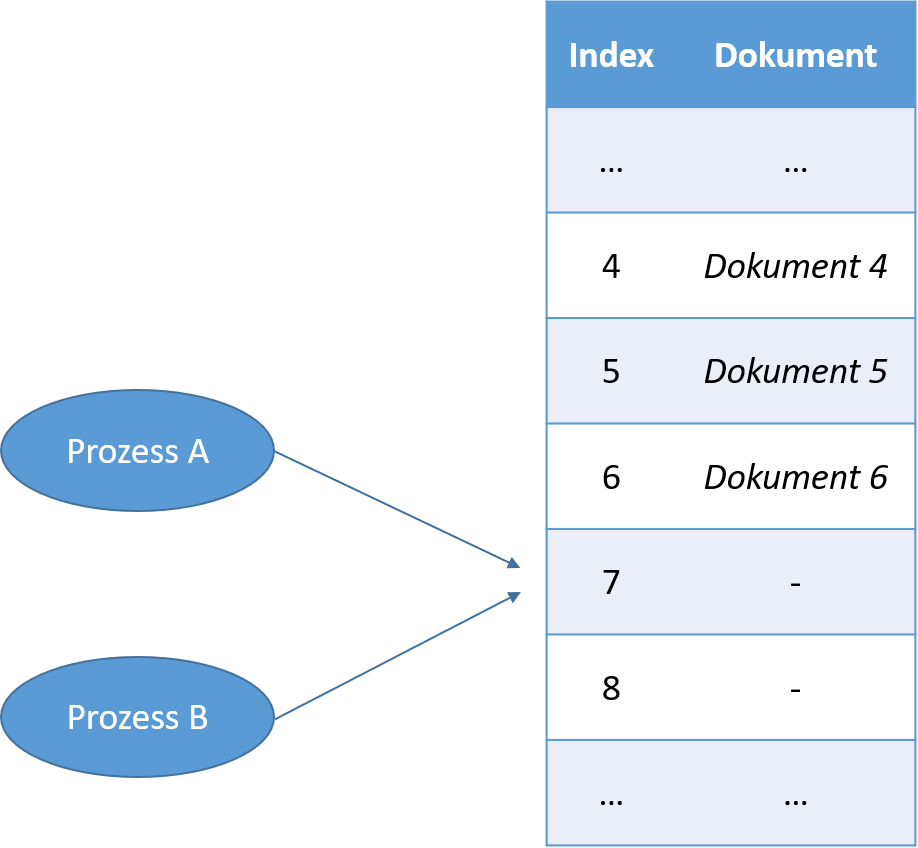
\includegraphics[width=6cm]{Abbildungen/Zeitkritischer_Ablauf_Drucker_Spooler.png}
							\caption{Grafische Darstellung des Drucker-Spoolers als ein Beispiel für einen zeitkritischen Ablauf.}
							\label{fig:ZeitkritischerAblaufDruckerSpooler}
						\end{figure}
					
					\item[Kritischer Abschnitt]

						Nun wird die in Punkt \ref{ZeitkritischerAblauf} genannte Problematik nicht mehr abstrakt, sondern auf Ebene des Quellcodes der beteiligten Prozesse betrachtet.\\
						Solange die Prozesse auf keine gemeinsamen Ressourcen zugreifen, kann es zu keinen zeitkritischen Abläufen kommen. Nur das lesende und schreibende Zugreifen auf Ressourcen, auf welche mehrere Prozesse Zugriff besitzen, kann zu dieser Art von Problemen führen. Die Teile eines Programmes, in welchen ein Zugriff auf solche gemeinsam genutzten Ressourcen erfolgt, nennt man \textbf{kritische Regionen} oder auch \textbf{kritische Abschnitte}.\\
						Um dieses Problem zu lösen, muss man auf ein Konzept von höchster Wichtigkeit in Zusammenhang mit dem parallelen Programmierparadigma, nämlich auf die \textit{Prozess-Synchronisation}, zurückgreifen.  \cite{ModerneBetriebssysteme}
				\end{description}
				
			\subsubsection{Verklemmung (Deadlock)}
			
				Bei Rechnersystemen gibt es meist Ressourcen, die gleichzeitig nur einem Prozess zugewiesen werden können. Wenn zwei Prozesse gleichzeitig zwei Dokumente mit dem selben Drucker drucken möchten, so ist nicht klar, wie der Drucker vorgehen sollte und er wird höchstwahrscheinlich nur unbrauchbare Dokumente drucken. Aus diesem Grund sind Betriebssysteme dazu in der Lage, Ressourcen für eine bestimmte Zeit nur einem einzigen Prozess zuzuweisen.\\
				Nun existieren aber Situationen, in welchen ein Prozess mehrere (also \textit{n}) Ressourcen gleichzeitig benötigt, um weiterarbeiten zu können. Das bedeutet, dass er erst aus dem Blockiert- in den Bereit- bzw. Aktiv-Zustand gelangen kann, sobald alleinig dem Prozess alle \textit{n} Ressourcen zur Verfügung stehen. Ein Beispiel hierfür ist ein Prozess A, der ein Dokument einscannen und gleichzeitig auf dem Bildschirm den aktuellen Scan-Status anzeigen möchte. Um arbeiten zu können, benötigt dieser Prozess folglich die beiden Ressourcen Scanner und Bildschirm.\\
				Im folgenden Szenario kommt es nun zu einem Problem. Auf einem System laufen zwei Prozesse A und B, wobei der Prozess B gerade den Scanner für sich reserviert hat und damit arbeitet. Sobald nun Prozess A an die Reihe kommt, fordert er die beiden Ressourcen Bildschirm und Scanner an. Da der Prozess B den Scanner gerade verwendet und für sich reserviert hat, kann der Prozess A nicht arbeiten, da er wie bereits erwähnt sowohl den Bildschirm als auch den Scanner benötigt, jedoch nur den Bildschirm erhält. Der Prozess A gelangt nun folglich in den Blockiert-Zustand und wartet, bis die Ressource Scanner freigegeben wird. Fordert nun der Prozess B auch noch den Bildschirm an und gibt den Scanner nicht frei, da er beispielsweise noch mit einem Scan-Vorgang beschäftigt ist, so geht auch der Prozess B in den Blockiert-Zustand, da er nicht alle von ihm angeforderten Ressourcen erhält. Ab diesem Zeitpunkt befinden sich beide Prozesse in einem Szenario, in welchem sie sich gegenseitig blockieren, sodass nie wieder einer der beiden den Blockiert-Zustand verlassen wird. Eine solche Situation nennt man \textit{Deadlock} oder auch \textit{Verklemmung}. \cite{DeadlockWikipedia}\\
				Solche Deadlocks können auch zwischen mehr als zwei Prozessen und mit mehr als zwei Ressourcen entstehen. Die Situation einer Verklemmung bei zwei Prozessen A und B und zwei Ressourcen 1 und 2 ist in der Abbildung \ref{fig:DeadlockSchema} schematisch dargestellt.
				
				\begin{figure}
					\centering	
					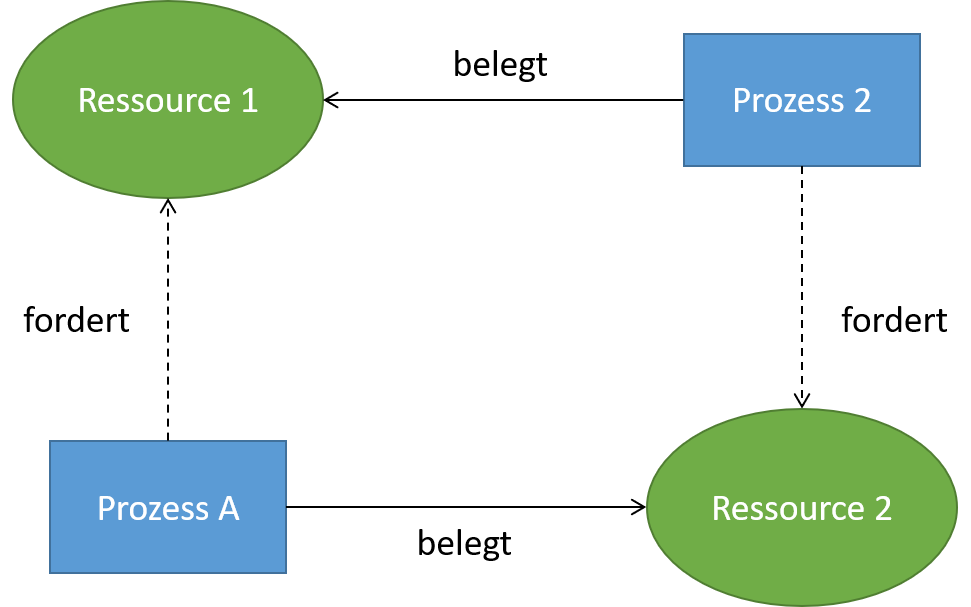
\includegraphics[width=8cm]{Abbildungen/Deadlock_Schema.png}
					\caption{Grafische Darstellung eines Deadlocks bei zwei Prozessen A und B und zwei Ressourcen 1 und 2.}
					\label{fig:DeadlockSchema}
				\end{figure}
			
				Formal lässt sich der Begriff Deadlock laut Andrew S. Tanenbaum wie folgt definieren:
				
				\begin{quote}
					\textit{Eine Menge von Prozessen befindet sich in einem Deadlock-Zustand, wenn jeder Prozess aus der Menge auf ein Ereignis wartet, das nur ein anderer Prozess aus der Menge auslösen kann. \cite{ModerneBetriebssysteme}}
				\end{quote}
				
				Alle Prozesse dieser Menge befinden sich somit im blockierten Zustand und werden die Ereignisse, auf welche die anderen Prozesse dieser Menge warten, nie auslösen können. \cite{ModerneBetriebssysteme}
								
			\subsubsection{Starvation (Aushungerung)}
			
				Ein weiteres bekanntes Problem bei der parallelen Verarbeitung ist die \textbf{Starvation}, im Deutschen auch oft als \textit{Aushungerung} oder \textit{Verhungerung} bekannt. Dieser Sachverhalt ist eng mit Deadlocks verwandt, darf allerdings nicht einem Deadlock gleichgesetzt werden.\\
				Dabei wird ein System angenommen, auf welchem mehrere Prozesse laufen, die theoretisch ständig Ressourcen anfordern können. Nun können Situationen auftreten, in welchen gleichzeitig mehrere Prozesse dieselbe Ressource anfordern. In diesem Fall muss das Betriebssystem einen Prozess nach einem bestimmen Verfahren aus der Liste von anfragenden Prozessen auswählen und diesem dann die Ressourcen zuteilen. Bei der Wahl des Auswahlverfahren ist allerdings Vorsicht geboten, da auch Verfahren, die zunächst gerecht erscheinen, dazu führen können, dass ein Prozess niemals arbeiten kann, weil er die geforderte Ressource nie erhält, obwohl er sich nicht in einem Deadlock befindet.\\
				Ein alltägliches Beispiel wäre die Zuweisung eines Druckers an Prozesse, die ein Dokument drucken möchten. Um keinen Deadlock zu erzeugen, wählt das System immer dann, wenn mehrere Prozesse gleichzeitig den Drucker anfordern, denjenigen Prozess aus, der das kleinste Dokument (mit der kleinsten Dateigröße) drucken will. Dieses Auswahlkriterium scheint gerecht zu sein. Doch der Fehler wird klar, wenn man eine Situation annimmt, in welcher der Drucker ständig Aufträge von Prozessen erhält und ein Prozess eine extrem große Datei drucken möchte. Nach jedem vollendeten Druck betrachtet das System die Warteschlange von Prozessen, die ein Dokument drucken möchten, und wählt daraus den Prozess, der das kleinste Dokument drucken wird. Kommen nun dauernd neue, kurze Druckaufträge an, so werden diese immer vorgezogen und der Prozess, der die große Datei drucken möchte, wird niemals den Drucker zugewiesen bekommen. Unter diesen Umständen verhungert dieser Prozess, das bedeutet, dass er unendlich lange Zeit im blockierten Zustand auf die Zuteilung des Druckers warten muss, obwohl er sich nicht in einem Deadlock befindet.\\
				Verallgemeinert kann eine Starvation immer dann auftreten, wenn an Prozesse nach einem gewissen Priorisierungs-System Ressourcen zugewiesen werden. Gibt es dann einen Prozess, der eine sehr niedrige Priorität besitzt und werden dauernd Ressourcenanfragen von Prozessen mit höheren Prioritäten gestellt, so wird der Prozess mit der sehr niedrigen Wichtigkeit unendlich lange auf die Zuteilung der Ressource warten und verhungern. \cite{ModerneBetriebssysteme}
			
		\subsection{Lösungen zu den Problemen der parallelen Verarbeitung}
		
			\subsubsection{Lösungen zum zeitkritischen Ablauf}
			
				Betrachtet man das Problem eines zeitkritischen Ablaufes auf einer abstrakten Ebene, so müssen Mechanismen gefunden werden, um sicherzustellen, dass von mehreren Prozessen gemeinsam genutzte Ressourcen gleichzeitig nur von einem einzigen Prozess schreibend und lesend verwendet werden dürfen. Dieser Sachverhalt wird als \textbf{wechselseitiger Ausschluss}, im Englischen \textbf{Mutual Exclusion} (kurz \textit{Mutex}) genannt, bezeichnet. Unter Verwendung dieses Verfahrens ist stets gewährleistet, dass nur ein Prozess eine gemeinsam genutzte Ressource gleichzeitig verwenden kann und alle anderen Prozesse, die auch Zugriff auf diese Ressource erhalten möchten, werden so lange blockiert, bis der Prozess die Ressource nicht mehr nutzt. Dann darf der nächste Prozess allein diese Ressource nutzen. Das Ziel ist folglich, die Ausführung von Prozessen, die gemeinsame Ressourcen besitzen, so anzuordnen, dass mehrere Prozesse niemals gleichzeitig in ihren kritischen Bereichen sind. Wird dieses Ziel erreicht, so werden zeitkritische Abläufe vermieden. Befindet sich also ein Prozess A in seiner kritischen Region und ein Prozess B versucht ebenfalls, seine kritische Region zu betreten, so wird dieser scheitern. Der Prozess B muss vorübergehend "`schlafen gelegt"' werden, bis der Prozess A seine kritische Region verlässt.\\
				Laut Andrew S. Tanenbaum garantiert das Verhindern von zeitkritischen Abläufen allerdings noch nicht das effiziente Zusammenarbeiten mehrerer parallel ablaufenden Prozesse, die über gemeinsame Ressourcen verfügen. Laut ihm müssen die folgenden vier Bedingungen erfüllt sein, um eine hochwertige Lösung zu erzielen:\\
				
				\begin{enumerate}
					\item Mehrere Prozesse dürfen sich nie gleichzeitig in ihren kritischen Regionen, in welchen der Zugriff auf die gemeinsame Ressource erfolgt, befinden.
					\item Es dürfen keine Annahmen über die Geschwindigkeit und die Anzahl der CPUs gemacht werden.
					\item Kein Prozess, der sich außerhalb seiner kritischen Region befindet, darf andere Prozesse blockieren. Das bedeutet, dass ein Prozess A nur einen anderen Prozess B blockieren darf, wenn der Prozess A gerade die gemeinsame Ressource nutzt und der Prozess B sie gerne nutzen möchte.
					\item Kein Prozess soll ewig darauf warten müssen, in seinen kritischen Bereich einzutreten. Somit muss die Warteschlange von Prozessen, die die gemeinsam genutzte Ressource verwenden möchten, gerecht koordiniert werden. \cite{ModerneBetriebssysteme}
				\end{enumerate}
				
				Der gegenseitige Ausschluss unter Verwendung von kritischen Regionen ist in der Abbildung \ref{fig:MutexKritischeRegionen} dargestellt. Diese Abbildung wurde dem Buch \textit{Moderne Betriebssysteme} von \textit{Andrew S. Tanenbaum}, welches sich im Literaturverzeichnis unter \cite{ModerneBetriebssysteme} finden lässt, entnommen und veranschaulicht den Vorgang grafisch.
				
				\begin{figure}
					\centering	
					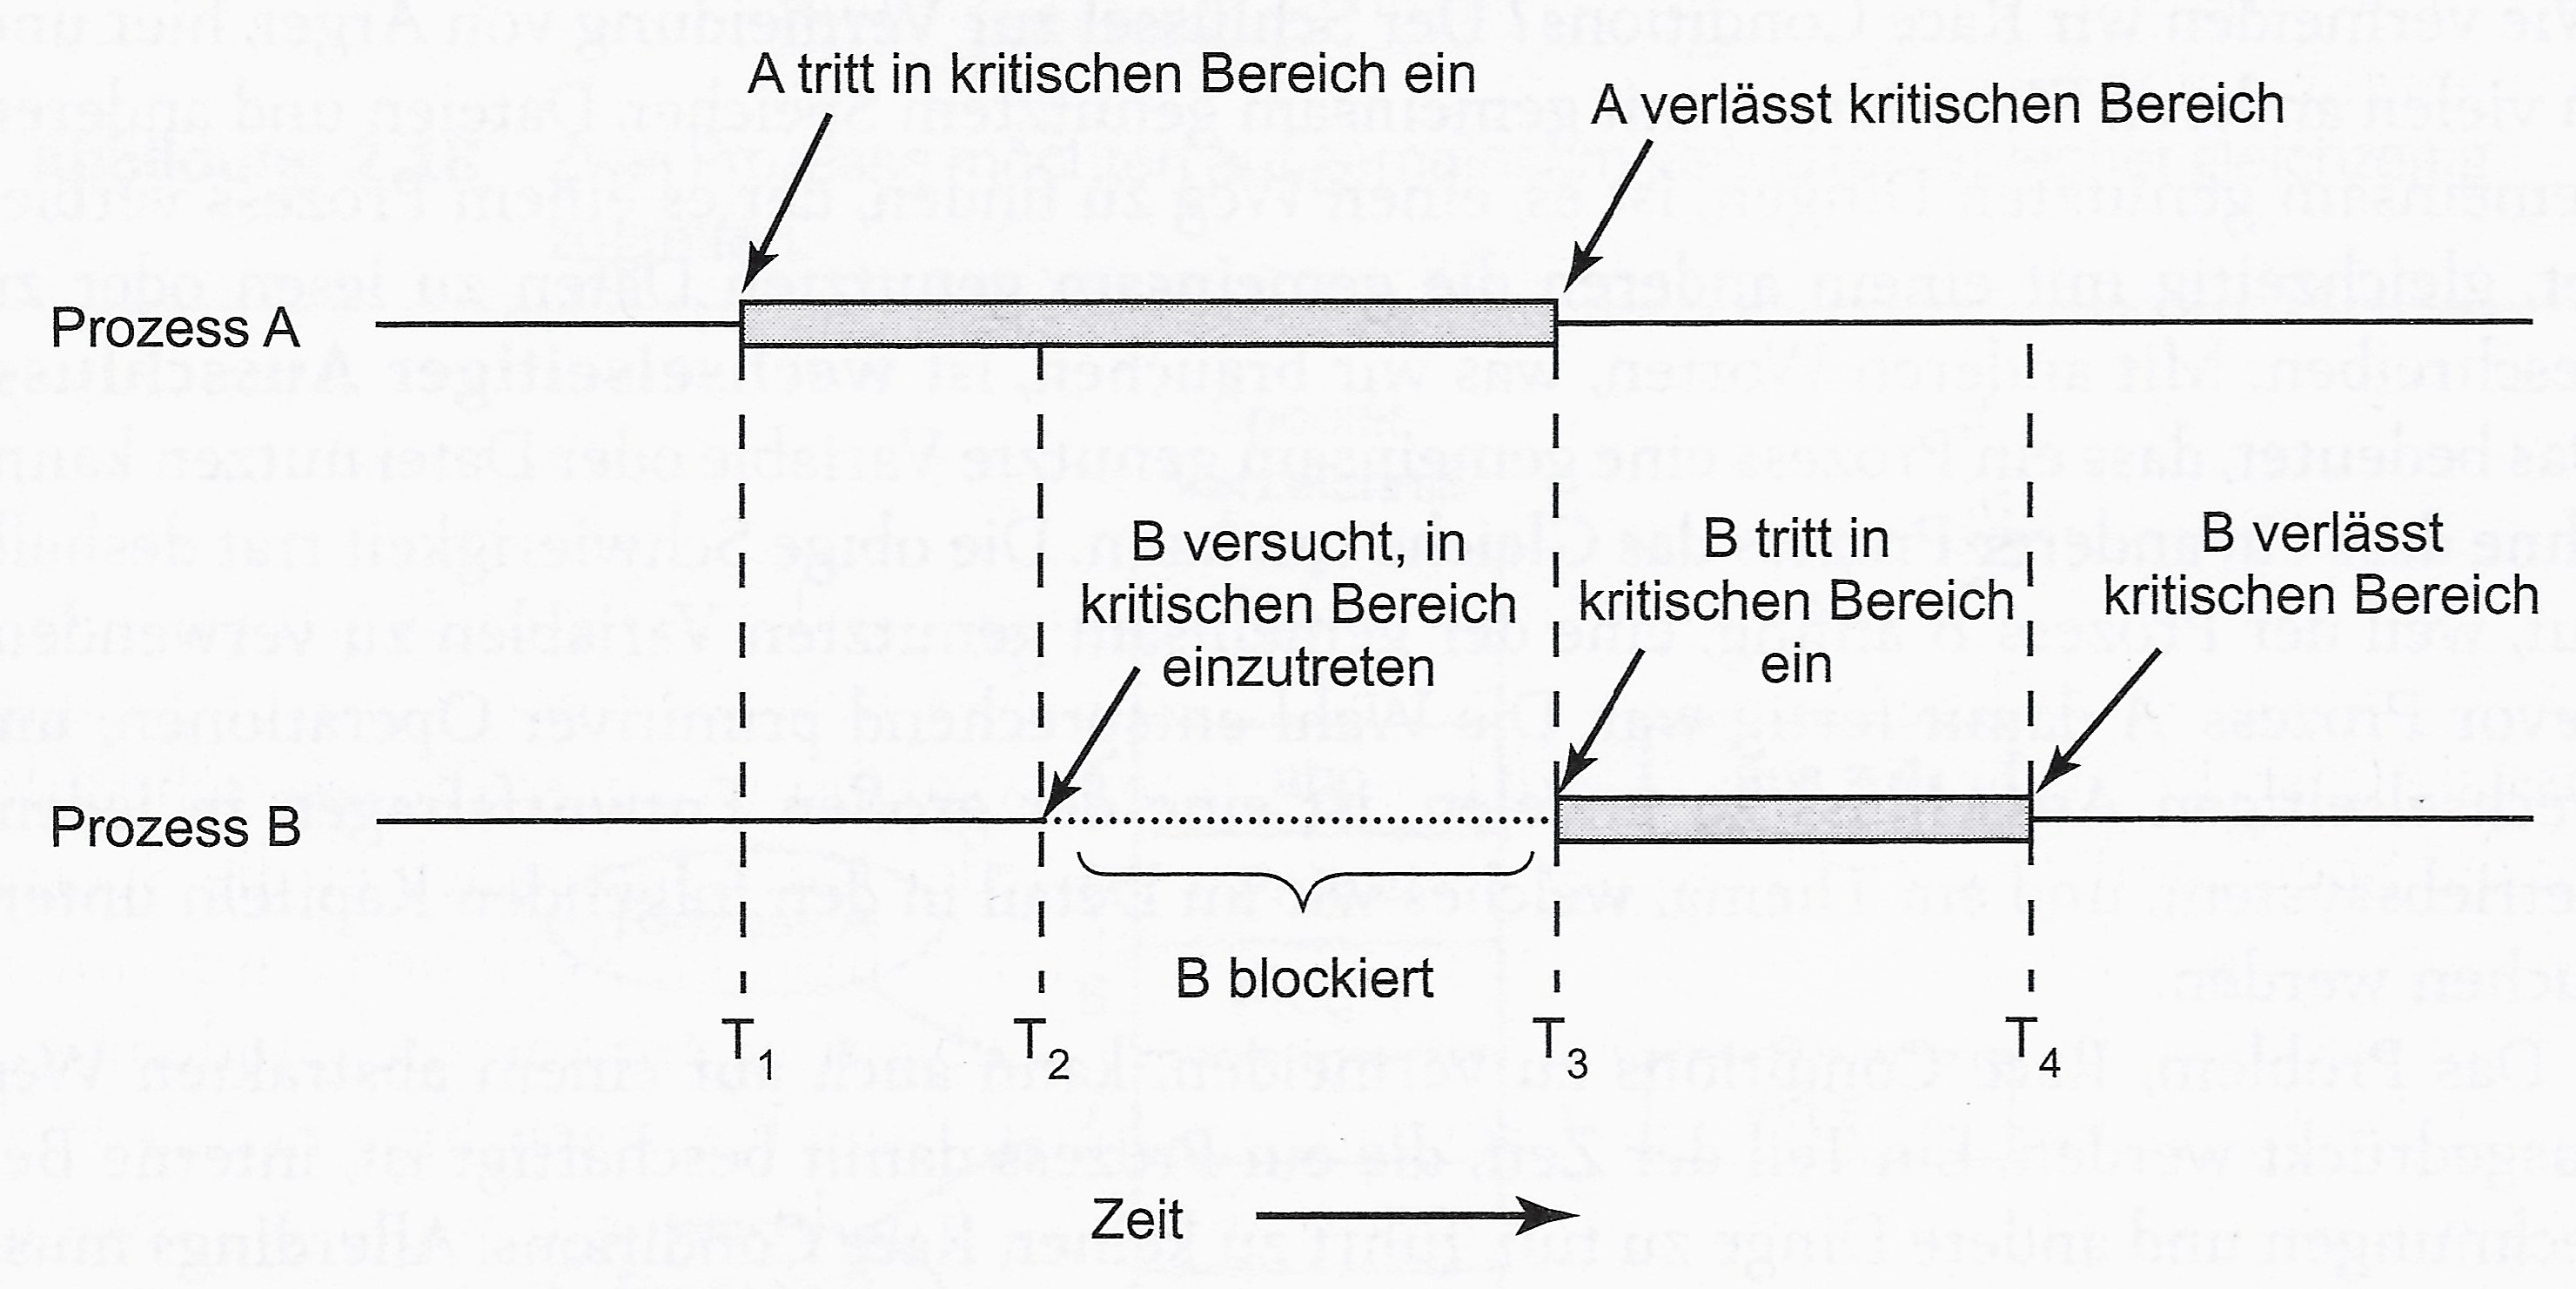
\includegraphics[width=11cm]{Abbildungen/Mutex_kritische_Regionen.jpg}
					\caption{Grafische Darstellung des wechselseitigen Ausschlusses von zwei Prozessen unter der Verwendung von kritischen Regionen.}
					\label{fig:MutexKritischeRegionen}
				\end{figure}
				
				Um diesen wechselseitigen Ausschluss zu realisieren, wurden verschiedene Mechanismen entwickelt, wobei einige im Folgenden erläutert werden. Der Grundgedanke ist jedoch immer die Schaffung eines \textit{geregelten Zugriffs} auf die gemeinsame Ressource. \cite{ModerneBetriebssysteme}\\
				
				\begin{description}
					\item[Wechselseitiger Ausschluss durch Arbeiten mit Interrupts]
					
							Um zu verstehen, wie diese Realisierungsmöglichkeit funktioniert, muss zunächst klargestellt werden, wie Prozessen mitgeteilt wird, dass ihnen der Prozessor entrissen wird. Dies geschieht in der Regel durch sogenannte Interrupts, auch Unterbrechungen genannt. Durch Unterbrechungen wird die CPU also von einem Prozess zum nächsten "`weitergereicht"'. Die Idee besteht nun darin, die Unterbrechungen auszuschalten, sobald ein Prozess seine kritische Region betritt, und sie erst wieder einzuschalten, bevor er die Region verlässt. Durch die ausgeschalteten Unterbrechungen wird der Prozessor dem Prozess so lange ununterbrochen zur Verfügung stehen, bis er die kritische Region wieder verlässt. Somit kann der Prozess, der die kritische Region betritt, sicher sein, dass ihm kein anderer Prozess bei seinem Zugriff auf die gemeinsame Ressource stört oder in die Quere kommt.\\
							Dieser Ansatz klingt zwar einfach, mit ihm geht allerdings ein großes Risiko einher. Man gibt in diesem Fall einem Benutzerprozess die Macht, Unterbrechungen ein- und auszuschalten. Dies könnte von einem Prozess einfach missbraucht werden, denn schaltet er aus eigenem Antrieb die Interrupts nicht wieder ein, so bekommt nie wieder ein anderer Prozess außer er selbst die CPU.\\
							Ein weiteres Problem ist, dass dieses Verfahren nur auf einem Ein-Prozessor-System funktioniert. Falls die \textit{disable}-Anweisung, welche die Ausschaltung der Unterbrechungen bewirkt, auf einem Mehr-Prozessor-System mit mehr als einer CPU ausgeführt wird, so wirkt diese Anweisung nur auf der CPU, welche diese auch ausgeführt hat. Auf den anderen CPUs können die Prozesse problemlos weiterlaufen und auch auf die gemeinsame Ressource zugreifen.\\
							Aus obigen Gründen wird klar, dass das Ausschalten der Interrupts nicht eine ideale Lösung für die Realisierung eines wechselseitigen Ausschlusses darstellt. \cite{ModerneBetriebssysteme}
							
					\item[Wechselseitiger Ausschluss unter Verwendung von aktivem Warten]
					
						Die einfachsten Lösungen zur Realisierung einer Mutual Exclusion verwenden das sogenannte \textit{aktive Warten}. Ein solcher Lösungsansatz soll exemplarisch im Folgenden genannt werden.
					
						\begin{description}
							\item[Sperrung durch Variablen]
							
								Dieser Lösungsansatz geht von einer einzigen, gemeinsam von den um die gemeinsame Ressource konkurrierenden Prozessen zugreifbaren Sperr-Variable \textit{lock} aus, welche mit dem Wert 0 initialisiert ist. Ist \textit{lock = 0}, so ist die Sperre nicht gesetzt und keiner der Prozesse befindet sich gerade in seiner kritischen Region. Ist hingegen \textit{lock = 1}, so ist die Sperre gesetzt, was bedeutet, dass sich gerade einer der Prozesse in seiner kritischen Region befindet und somit kein anderer seine kritische Region betreten darf.\\
								Will ein Prozess in seinen kritischen Bereich eintreten, so überprüft er zunächst den Zustand der Sperr-Variablen. Ist die Sperr-Variable gleich 0, so setzt der Prozess die Variable auf 1 und betritt die kritische Region. Nach dem Verlassen der Region setzt der Prozess die Variable dann wieder auf 0, um zu signalisieren, dass sich kein Prozess aktuell in seinem kritischen Bereich befindet. Falls die Sperre beim Überprüfen jedoch gleich 1 wäre, so würde der Prozess einfach warten, bis sie gleich 0 wird.\\
								Leider funktioniert dieser Ansatz nicht, da auch die Variable \textit{lock} wiederum eine gemeinsam genutzte Ressource darstellt und es deshalb auch in Zusammenhang mit dieser gemeinsam genutzten Variable zu zeitkritischen Abläufen kommen kann. Das folgende Beispiel soll das Problem dieser Lösung illustrieren. Zunächst erreicht Prozess A seine kritische Region, überprüft den Zustand der Variable \textit{lock} und stellt fest, dass sie gleich 0 ist. Er geht also davon aus, dass kein Prozess aktuell die gemeinsame Ressource nutzt. Bevor er den kritischen Bereich jedoch für sich sperren kann, also \textit{lock = 1} setzen kann, wird ihm der Prozessor entrissen und der Prozess B bekommt die CPU. Auch dieser erreicht seinen kritischen Bereich und überprüft die Sperr-Variable. Diese ist immer noch auf 0, weshalb auch der Prozess B davon ausgeht, dass die gemeinsame Ressource gerade von keinem anderen Prozess verwendet wird. Jetzt setzt der Prozess B die Sperr-Variable auf 1 und betritt die kritische Region. Sobald nun der Prozess A wieder die CPU erhält, setzt dieser auch nochmals die Variable auf 1 und betritt die Region. Beide Prozesse werden nun also gleichzeitig in ihren kritischen Regionen ausgeführt, weshalb dieses Verfahren zur Realisierung von wechselseitigem Ausschluss fehlschlägt.\\
								Um eine funktionierende Lösung zu erreichen, muss der Zugriff auf die gemeinsame Variable selbst koordiniert werden. \cite{ModerneBetriebssysteme}
								
							\item[Test-and-Set-Anweisung]
							
								Diese Lösung baut auf dem vorher genannten Konzept einer Sperr-Variable auf, löst allerdings die genannte Problematik durch Unterstützung seitens der Hardware. Viele Prozessoren haben im Befehlssatz eine Anweisung mit dem Namen \textit{Test and Set Lock}, kurz auch \textit{Test and Set} oder \textit{TSL} genannt. Dies ist eine Instruktion auf Maschinencode-Ebene, die im Allgemeinen die folgende Form aufweist:
								
								\lstinputlisting[emph={TSL}, emphstyle=\bfseries, breaklines=true]{Quellcode/TSL_Syntax.asm}
								
								Dieser Befehl liest den Inhalt des Speicherwortes\footnote{Ein Datenwort, Speicherwort oder einfach nur Wort ist die Grundverarbeitungsdatengröße bei einem Computer. \cite{DatenwortWikipedia}} \textit{LOCK} aus und speichert den ausgelesenen Wert ins Register \textit{REGISTER}. Anschließend speichert der Befehl einen Wert ungleich 0 an die Speicheradresse von \textit{LOCK}.\\
								Das Lesen und Schreiben des Speicherwortes wird dabei als garantiert hardwareseitig unteilbare, also atomare, Operation durchgeführt. Dies bedeutet, dass kein anderer Prozess auf das Speicherwort zugreifen kann, bis die Anweisung beendet ist. Des Weiteren wird während der Ausführung dieses Befehls auch der Speicherbus\footnote{Der Speicherbus verbindet die CPU (oder einen Speichercontroller) mit dem Hauptspeicher. \cite{SpeicherbusWikibooks}} gesperrt. Dies bedeutet, dass auch - falls auf einem Mehr-Prozessor-System gearbeitet wird - anderen Prozessen, welche auf anderen CPUs laufen, der Zugriff auf den Speicher verwehrt bleibt, bis die Instruktion fertig abgearbeitet ist.\\
								Nun wird wieder, wie beim Lösungsversuch \textit{Sperrung durch Variablen} eine gemeinsame Variable \textit{lock} verwendet, um den Zugriff auf die gemeinsam genutzte Ressource zu koordinieren. Wenn \textit{lock = 0} gilt, kann jeder beliebige Prozess die \textit{TSL}-Anweisung verwenden, um die Sperr-Variable frei von zeitkritischen Abläufen auf 1 zu setzen. Dieser Prozess kann dann seinen kritischen Bereich betreten und auf die gemeinsame Ressource zugreifen. Ist die erledigt, so kann die Variable mit der gewöhnlichen Maschinencode-Instruktion \textit{MOVE}\footnote{Der \textit{MOVE}-Befehl (oft auch \textit{MOV}-Befehl) kopiert einen Wert, der entweder direkt angegeben wird oder in einem Register gespeichert sein kann, in ein Register. \cite{MoveBefehlWikibooks}} wieder auf 0 gesetzt werden, da sich bei diesem Vorgang kein zeitkritischer Ablauf ergibt.\\
								Auf Assembler-Ebene lassen sich nun zwei Unterprogramme \textit{enterRegion} und \textit{leaveRegion} schreiben. Das \textit{enterRegion}-Unterprogramm muss dabei folgende Funktionalität unterstützen: Zunächst muss die \textit{TSL}-Anweisung aufgerufen werden, wodurch der alte Wert der Sperr-Variable \textit{lock} in einem Register gespeichert und \textit{lock} auf 1 gesetzt wird. Nun wird der von der \textit{TSL}-Anweisung in das Register gespeicherte Wert mit der Zahl 0 verglichen. Ist der Wert im Register ungleich 0, so war die Sperre bereits gesetzt und das Unterprogramm springt zurück zum Start, wodurch die Prozedur von Neuem beginnt. Sobald der Prozess, der sich gerade im kritischen Bereich befindet, den Bereich verlässt und die Sperr-Variable wieder auf 0 setzt, so wird auch im Register der Wert 0 stehen und die Schleife, in der sich das Unterprogramm befand, beendet. Dann beendet sich das Unterprogramm mit der für den Prozess gesetzten Sperre und kehrt zum Aufrufspunkt zurück. Nun kann die kritische Region durchlaufen werden. Sobald dies geschehen ist, kann der Prozess das Unterprogramm \textit{leaveRegion} aufrufen. In diesem wird die Sperre aufgelöst, indem einfach der Wert 0 in die gemeinsame Variable \textit{lock} gespeichert wird. Hier ist kein Aufruf der \textit{TSL}-Anweisung nötig.
								Um das soeben Erklärte zu veranschaulichen, wurden die beiden Unterprogramme in einer Pseudo-Assemblersprache abgefasst und im Folgenden aufgelistet.
		
								\lstinputlisting[emph={TSL, BNE, MOV, RET}, emphstyle=\bfseries, breaklines=true]{Quellcode/TSL_enterRegion_leaveRegion.asm}
								
								Im Unterprogramm \textit{enterRegion} erkennt man, dass der Inhalt des Speicherwortes \textit{LOCK} solange überprüft wird, bis eine Bedingung eintritt, in diesem Fall, dass dieser Wert gleich 0 ist. Solange \textit{LOCK} ungleich 0 ist, wird in einer Schleife somit dauernd der Wert überprüft. Das dauernde Überprüfen einer Variable, bis sie einen gewünschten Wert annimmt, nennt man \textbf{aktives Warten}. Prozesse sollten im Allgemeinen allerdings nicht aktiv warten, da somit die CPU-Zeit, die dem jeweiligen wartenden Prozess zugeteilt wird, nur durch Überprüfen einer Bedingung verschwendet wird. Aktiv gewartet werden soll, wenn überhaupt, nur, falls kurze Wartezeiten zu erwarten sind. Wird aktives Warten eingesetzt, so wird die verwendete Sperr-Variable \textit{Spinlock} genannt. Ein Spinlock kann die Programmausführung stark verlangsamen, wenn mehr Prozesse bzw. Threads als CPUs im System vorhanden sind. \cite{ModerneBetriebssysteme} \cite{SpinlockWikipedia}\\
								Nun kann das vorherige Problem gelöst werden. Vor dem Betreten einer kritischen Region ruft der Prozess \textit{enterRegion} auf. Dieses Unterprogramm wartet wie bereits erläutert aktiv auf das Freiwerden der gemeinsamen Ressource, sperrt die Ressource für den aufrufenden Prozess und kehrt dann zum Aufrufspunkt zurück. Nun kann der Prozess ungestört seine Arbeit im kritischen Bereich verrichten. Sobald dies geschehen ist, ruft der Prozess \textit{leaveRegion} auf, welches die Sperr-Variable \textit{LOCK} auf 0 setzt und die Ressource somit wieder freigibt.\\
								Dieses Verfahren zur Realisierung von gegenseitigem Ausschluss funktioniert garantiert korrekt, bringt allerdings des Nachteil des aktiven Wartens, also des Verschwendens von CPU-Zeit, mit sich. Aus diesem Grund werden nun noch weitere Methoden zur Realisierung von Mutual Exclusion erläutert. \cite{ModerneBetriebssysteme}
						\end{description}
				
					\item[Wechselseitiger Ausschluss unter Verwendung von Semaphoren]
					
						Die vorgestellte Lösung durch Einsatz der TSL-Anweisung funktioniert zwar auf den ersten Blick korrekt, verschwenden aber unnötig CPU-Zeit, was im Allgemeinen nicht geschehen sollte.\\
						Es gibt aber sogar Situationen, in welchen dieser Lösungsansatz versagt. Der Fehler wird klar, wenn man ein Rechner-System annimmt, auf welchem zwei Prozesse H und N laufen, wobei der Prozess H ein hohe und der Prozess N eine niedrige Priorität aufweist. Bei Einsatz von prioritätenbasiertem Scheduling, welches unter Punkt \ref{ProzessScheduling} erläutert wurde, ist klar, dass der Prozess H auf Grund seiner hohen Priorität immer dann laufen darf, wenn er sich im bereiten Zustand befindet.\\
						Nun kann es zu einer Situation kommen, in welcher der Prozess N seinen kritischen Bereich betritt und somit die Ressource exklusiv nutzt. Gelangt der Prozess H in der Zwischenzeit in den Bereit-Zustand, beispielsweise weil ein Ereignis, auf das er gewartet hat, eingetreten ist, so erhält der Prozess H die CPU. Will nun der Prozess H auch auf die Ressource zugreifen, so beginnt dieser mit aktivem Warten. Da nun der Prozess H dauernd aktiv ist und somit dem Prozess N nie die CPU zugeteilt wird, erhält er auch nie die Möglichkeit, die Ressource und die Sperre freizugeben. Als Ergebnis bleibt der Prozess H für immer in seiner aktiv wartenden Schleife. Diese Problematik wird als das Problem der Prioritätsumkehrung bezeichnet.\\
						Um die genannten Schwächen der bisherigen Probleme zu umgehen, wurde deshalb ein neuer Ansatz entwickelt. In diesem Fall gibt es zwei Befehle, \textit{Sleep} und \textit{Wakeup}. Der Aufruf von \textit{Sleep} legt den aufrufenden Prozess schlafen, das heißt, er wird blockiert, bis er von einem anderen Prozess wieder aufgeweckt wird. Der Aufruf von \textit{Wakeup} muss dabei von einem anderen Prozess geschehen und diesem Befehl muss ein eindeutiger Bezeichner des schlafenden Prozesses übergeben werden. Der schlafende Prozess kommt dann vom blockierten wieder in den bereiten Zustand. Somit wird ein Prozess blockiert, wenn er seinen kritischen Bereich nicht betreten darf. Dadurch wird keine unnötige CPU-Zeit verschwendet.\\
						Ein bekanntes Problem, welches oft mit diesen beiden Befehlen gelöst wird, ist das sogenannte \textit{Erzeuger-Verbraucher-Problem}. Aus diesem Grund wird dieses Problem zunächst erklärt und dann unter Einsatz von \textit{Sleep} und \textit{Wakeup} gelöst. \cite{ModerneBetriebssysteme}
						
						\begin{description}
							\item[Das Erzeuger-Verbraucher-Problem]
							
								In diesem Problem, das oft auch im Englischen \textit{Producer-Consumer-Problem} genannt wird, geht man von zwei parallel ablaufenden Prozessen aus, die beide unterschiedliche Aufgaben erledigen und als gemeinsame Ressource einen Puffer mit fester, beschränkter Größe besitzen. Der Prozess E wird auch Erzeuger genannt. Er ist dazu in der Lage, Informationen in den Puffer zu legen. Der Prozess V, also der Verbraucher, kann die Informationen wieder aus dem Puffer herausnehmen. Das Erzeugen und Verbrauchen geschieht jeweils an zufälligen Zeitpunkten. Des Weiteren gibt es eine Variable \textit{count}, welche die aktuelle Anzahl an Informations-Elementen im Puffer speichert. Sie ist zunächst mit 0 initialisiert.\\
								Der Erzeuger prüft vor dem Ablegen eines neuen Elementes in den Puffer, ob noch freier Platz im Puffer vorhanden ist. Ist dies der Fall, so inkrementiert er die Variable \textit{count} und legt ein Element in den Puffer. Ist der Puffer voll, so legt sich der Erzeuger durch Aufruf von \textit{Sleep} schlafen. Der Verbraucher prüft vor der Entnahme eines Elementes, ob der Puffer nicht leer ist. Ist dies nicht der Fall, so dekrementiert er die Variable \textit{count} und entnimmt ein Element aus dem Puffer. Befindet sich kein Element im Puffer, so legt sich der Verbraucher durch Aufruf von \textit{Sleep} schlafen. Stets, wenn der Erzeuger ein Element in den Puffer legt und selbiger zuvor leer war, wird der Verbraucher durch Aufruf von \textit{Wakeup} geweckt. Umgekehrt verhält es sich genauso: Immer, wenn der Verbraucher ein Element aus dem Puffer entfernt, und selbiger zuvor voll war, wird der Erzeuger durch Aufruf von \textit{Wakeup} geweckt.\\
								Ein reales Beispiel, bei welchem das Erzeuger-Verbraucher-Problem auftreten kann, sind das Konzept von \textit{Pipes} in UNIX. Dabei erzeugt ein Prozess Daten, die ein anderer Prozess weiterverarbeitet. \cite{ModerneBetriebssysteme}\\
								\textit{Andrew S. Tanenbaum} zeigt in seinem Buch \textit{Moderne Betriebssysteme}, welches sich im Literaturverzeichnis unter \cite{ModerneBetriebssysteme} finden lässt, eine intuitive Lösung des Erzeuger-Verbraucher-Problems in der Programmiersprache C, das allerdings einen gravierenden Fehler enthält, der zu einem zeitkritischen Ablauf führt. Das Programm ist im Folgenden dargestellt. Anzumerken ist, dass es sich hierbei um Pseudocode handelt, da die im Programm aufgerufenen Funktionen nicht zur Standard-C-Programmiersprache gehören. \cite{ModerneBetriebssysteme}
								
								\lstinputlisting[language=C, breaklines=true]{Quellcode/Erzeuger-Verbraucher-Problem_mit_zeitkritischem_Ablauf.c}
								
								Kommen wir nun zum auftretenden Problem, also zum zeitkritischen Ablauf. Hierbei muss nochmals betont werden, dass beide Programme unabhängig voneinander in getrennten Prozessen ablaufen und ihnen die CPU jederzeit genommen werden kann.\\
								In der nun genannten Situation kommt es zu einem solchen zeitkritischen Ablauf. Im Moment befindet sich kein Element im Puffer und der Verbraucher hat gerade den Wert von \textit{count} ausgelesen und gesehen, dass er gleich 0 ist. Im Programm will der Verbraucher nun in die \textit{if}-Verzweigung einbiegen, doch genau in diesem Moment wird ihm die CPU entrissen und der Erzeuger kommt an die Reihe. Dieser erzeugt ein Element, fügt es in der Puffer ein, inkrementiert die Variable \textit{count} und bemerkt, dass die Variable nun den Wert 1 besitzt. Aus diesem Grund ist er der Ansicht, dass \textit{count} vor seiner Aktion gleich 0 war und der Verbraucher somit gerade schlafen muss. Aus diesem Grund führt der Erzeuger den \textit{wakeup}-Befehl aus, um den Verbraucher zu wecken. Doch genau hier kommt es zum Problem. Der Verbraucher verfügt zwar gerade nicht über die CPU, schläft aber noch nicht, da er die entsprechende Code-Zeile noch nicht ausführen konnte. Aus diesem Grund geht das \textit{wakeup}-Signal verloren. Sobald der Verbraucher nun eine Zeitscheibe erhält, biegt der Verbraucher in die \textit{if}-Verzweigung ein, in welche er schon vor dem Entreißen der CPU hinein springen wollte. In dieser Verzweigung findet der Verbraucher den \textit{sleep}-Befehl vor und geht schlafen. Nun wird der Erzeuger den Puffer so lange weiter auffüllen, bis er voll ist, und dann im glauben, dass der Verbraucher wach ist (was aber nicht der Fall ist), ebenfalls schlafen gehen. Als Ergebnis schlafen sowohl der Erzeuger, als auch der Verbraucher für immer. \cite{BetriebssystemeNetzmafia}\\
								Das grundlegende Problem in diesem Beispiel ist also, dass ein Aufweck-Signal, das an einen nicht schlafenden Prozess geschickt wird, verhallt und damit verloren geht. Dies ließe sich allerdings korrigieren, indem man ein sogenanntes \textit{Weckruf-Warte-Bit} einführen würde. Wenn ein Weckruf an einen Prozess gesendet wird, der aber noch gar nicht schläft, dann wird dieses Bit gesetzt. Sobald der Prozess dann schlafen gehen möchte, so wird dieses Bit gelöscht und der Prozess bleibt aber wach, da er durch das gesetzte Bit schon ein \textit{wakeup}-Signal erhalten hat, das seinen noch nicht begonnenen Schlaf schon im Vorherein beendet. Das Weckruf-Warte-Bit würde dem Verhallen des \textit{wakeup}-Signals entgegenwirken.\\
								Doch ein solches Bit löst das Problem nur in diesem Fall. Sobald mehr Prozesse involviert sind, reicht ein Bit nicht mehr aus. Nun könnte man noch weitere solche Weckruf-Warte-Bits hinzufügen, aber das Problem wird damit nicht allgemein und auch nicht elegant gelöst.
								Aus diesem Grund wird nun eine elegante Lösung vorgestellt. \cite{ModerneBetriebssysteme}
								
							\item[Semaphoren]
							
								Im Jahr 1965 schlug Edsger W. Dijkstra\footnote{Edsger Wybe Dijkstra (1930 - 2002) war ein niederländischer Informatiker. \cite{DijkstraWikipedia}} einen neuen Lösungsansatz vor. Seine Lösung geht von einer ganzzahligen Variable aus, welche die Anzahl von Weckrufen für die zukünftigen Aufweckungen speichert. Dijkstra schlug in diesem Zusammenhang für diese Variable eine neue Datenstruktur vor, welche er Semaphor\footnote{Das Wort \textit{Semaphor} ist dem Altgriechischen entlehnt und bedeutet \textit{Signalgeber}. \cite{SemaphorWikipedia}} nannte. Falls ein Semaphor den Wert 0 besitzt, so bedeutet dies, dass aktuell keine Weckrufe gespeichert sind. Ist ihm jedoch ein positiver Wert \textit{n} zugeordnet, so bedeutet dies, dass aktuell \textit{n} Weckrufe ausständig sind.\\
								Des Weiteren geht Dijkstra von zwei Operationen aus, welche er \textit{down} und \textit{up} nannte und die jeweils Verallgemeinerungen von \textit{sleep} und \textit{wakeup} darstellen. Die \textit{down}-Operation prüft, ob der Wert des Semaphors größer als 0 ist. Ist dies der Fall, so wird der Wert dekrementiert, um einen gespeicherten Weckruf zu verbrauchen. Falls der Wert hingegen 0 beträgt, so wird der Prozess schlafen gelegt, da kein Weckruf gespeichert wurde und der Prozess somit tatsächlich schlafen gehen muss. Dieser Prozess wird schlafen gelegt, ohne die \textit{down}-Operation vollständig ausführen zu können. Die Überprüfung des Wertes des Semaphors, die Modifikation desselben und auch das Schlafenlegen des Prozesses sind einzelne, unteilbare, atomare Aktionen. Das bedeutet, dass, wenn ein Prozess eine Operation auf einem Semaphor ausführt, kein anderer Prozess auf diesen zugreifen darf. Diese Eigenschaft ist unabdingbar, da auch der Semaphor wiederum eine gemeinsame Ressource darstellt und es ansonsten auch innerhalb der \textit{down}-Operation wieder zu zeitkritischen Abläufen kommen könnte. Die \textit{up}-Operation inkrementiert den Wert des Semaphors, um einen neuen gespeicherten Weckruf anzuzeigen. Falls es zum Zeitpunkt des Aufrufes einer \textit{up}-Operation Prozesse geben sollte, die wegen des Semaphors schlafen und somit in ihrer \textit{down}-Operation "`feststecken"', wird einer der schlafenden Prozesse anhand eines Kriteriums gewählt (z.B. durch Zufall) und aufgeweckt, wodurch dieser dann imstande ist, seine \textit{down}-Operation zu vollenden. Aus diesem Grund bleibt der Wert einer Semaphore, die vor dem Aufruf der \textit{up}-Operation den Wert 0 hatte und die für das Schlafen eines oder mehrerer Prozesse verantwortlich war, der Wert der Semaphore immer noch 0. Allerdings existiert dann ein Prozess weniger, der wegen der Semaphore schläft. Das Inkrementieren des Wertes des Semaphors und das Aufwecken eines Prozesses sind wieder einzelne, unteilbare Operationen. Anzumerken ist noch, dass Dijkstra ursprünglich die \textit{down}-Operation \textit{V}-Operation und die \textit{up}-Operation \textit{P}-Operation nannte. P und V sind sind die Initialen der niederländischer Wörter \textit{prolaag} und \textit{verhoog}. "`Verhoog"' ist niederländisch und bedeutet "`hochzählen"'. Das Wort "`Prolaag"' ist ein Kunstwort, das Dijkstra schuf, da das niederländische "`verlaag"' ("`herunterzählen"') ebenfalls mit "`v"' beginnt. \cite{SemaphorBorchert}  \cite{ModerneBetriebssysteme}\\

							\item[Lösung des Erzeuger-Verbraucher-Problems unter Verwendung von Semaphoren]
							
								Mit Semaphoren lässt sich nun das Problem des verhallenden Weckrufes lösen. \textit{Andrew S. Tanenbaum} zeigt in seinem Buch \textit{Moderne Betriebssysteme}, welches sich im Literaturverzeichnis unter \cite{ModerneBetriebssysteme} finden lässt, eine Lösung des Erzeuger-Verbraucher-Problems mit Semaphoren in der Programmiersprache C. Das Programm ist im Folgenden dargestellt. Anzumerken ist wieder, dass es sich auch hierbei um Pseudocode handelt, da die im Programm aufgerufenen Funktionen nicht zur Standard-C-Programmiersprache gehören.
								
								\lstinputlisting[language=C, breaklines=true]{Quellcode/Erzeuger-Verbraucher-Problem_Loesung_Semaphoren.c}
								
								Die obige Lösung verwendet drei Semaphoren für die Lösung des Problems. Der Semaphor \textit{empty} zaehlt die leeren Einträge im Puffer, weshalb er zunächst mit der Puffergröße initialisiert wird, während der Semaphor \textit{full} die vollen Einträge im Puffer speichert und aus diesem Grund mit 0 initialisiert wird. Der Semaphor \textit{mutex} nimmt dabei eine Sonderrolle ein. Er regelt die Zugriff auf den Puffer und realisiert somit Mutex, also wechselseitigen Ausschluss. Aus diesem Grund wird er zunächst mit 1 initialisiert, da nur ein Prozess gleichzeitig auf den Puffer zugreifen darf. Ein solcher Semaphor wird, da er nur die Werte 0 und 1 annehmen kann, auch als \textit{binärer Semaphor} bezeichnet. Falls jeder beteiligte Prozess vor dem Betreten seines kritischen Bereiches die \textit{down}-Operation auf diesem Semaphor ausführt und vor dem Verlassen die \textit{up}-Operation ebenfalls auf diesem binären Semaphor ausführt, so ist der gegenseitige Ausschluss sichergestellt.\\
								Wie bereits angedeutet wird im obigen Programm ein binärer Semaphor verwendet, um die exklusive Benutzung einer Ressource durch einen Prozess zu realisieren. Somit wird garantiert, dass immer nur ein Prozess gleichzeitig die gemeinsamen Ressourcen lesend und schreibend nutzen kann. Die anderen beiden Semaphoren, nämlich \textit{empty} und \textit{full}, werden für einen anderen Zweck verwendet. Die dienen der Synchronisation der beiden Prozesse in Bezug auf Ereignisse. Diese beiden Semaphoren sorgen dafür, dass der Erzeuger schlafen geht, wenn der Puffer voll ist, und auch dafür, dass der Verbraucher schlafen geht, wenn der Puffer leer ist. \cite{ModerneBetriebssysteme}
						\end{description}
					
					\item[Weitere bekannte Synchronisationsmechanismen und -probleme]
					
						Das Thema der Prozess-Synchronisation weist eine hohe Komplexität auf, weshalb es nicht möglich ist, sie im Rahmen dieser Arbeit vollständig zu beleuchten. Aus diesem Grund beschränkt sich diese Arbeit auf die obigen Konzepte. Der Vollständigkeit wegen werden allerdings noch weitere mögliche Lösungsansätze aufgezählt. Genauere Beschreibungen dieser Ansätze können dem Buch \textit{Moderne Betriebssysteme} von \textit{Andrew S. Tanenbaum}, welches sich im Literaturverzeichnis unter \cite{ModerneBetriebssysteme} finden lässt, entnommen werden.\\
						Neben der Synchronisation durch das Ausschalten der Interrupts, der Verwendung der \textit{Test-and-Set}-Anweisung und der Verwendung von Semaphoren gibt es noch einige weitere Mechanismen, wobei nur einige im Folgenden aufgezählt werden. \cite{ModerneBetriebssysteme}
						
						\begin{itemize}
							\item Strikter Wechsel
							\item Monitor
							\item Message Passing\footnote{Auf das Message-Passing-Programmiermodell wird im Kapitel \ref{MPI} eingegangen.}
							\item Barrieren \cite{ModerneBetriebssysteme}
						\end{itemize}
					
						Auch das vorgestellte Erzeuger-Verbraucher-Problem ist nur ein bekanntes Problem der Prozess-Synchronisationsproblematik. Auch hier gibt es eine Vielzahl von Problemen, die den Rahmen der Arbeit sprengen würden. Der Vollständigkeit wegen werden allerdings auch hier noch weitere klassische Probleme der IPC aufgezählt. Genauere Beschreibungen dieser Probleme und mögliche Lösungen können ebenfalls dem Buch \textit{Moderne Betriebssysteme} von \textit{Andrew S. Tanenbaum}, welches sich im Literaturverzeichnis unter \cite{ModerneBetriebssysteme} finden lässt, entnommen werden.
						Neben dem Erzeuger-Verbraucher-Problem gibt es noch einige weitere bekannte Probleme, wobei nur einige im Folgenden aufgezählt werden. \cite{ModerneBetriebssysteme}
						
						\begin{itemize}
							\item Das Problem der speisenden Philosophen
							\item Das Leser-Schreiber-Problem
							\item Das Problem des schlafenden Friseurs \cite{ModerneBetriebssysteme}
						\end{itemize}
				\end{description}
			
			\subsubsection{Lösungen zum Deadlock}
			
				Genauso wie zum Problem der zeitkritischen Abläufe, so wurde auch zu Deadlocks erhebliche Forschung betrieben und auch einige Lösungsansätze gefunden. Die Lösungen lassen sich dabei grob in zwei Gruppen einteilen: Das Beheben und das Verhindern von Deadlocks.  \cite{ModerneBetriebssysteme}
			
				\begin{description}
					\item[Behebung von Deadlocks]
						\label{BehebungDeadlocks}
						
						Ist ein Deadlock aufgetreten, so muss das System wieder in einen verklemmungsfreien Zustand gelangen, um ordnungsgemäß arbeiten zu können. Im Folgenden der mehrere Möglichkeiten behandelt, um einen Deadlock in einem System zu beheben.
						
						\begin{description}
							\item[Behebung von Deadlocks durch Unterbrechung]
							
								Eine Möglichkeit, einen Deadlock aufzuheben, besteht in der zeitweisen Suspendierung eines beteiligen Prozesses. Suspendieren bedeutet in diesem Fall, dass der Prozess als nicht ausführbar markiert wird. Somit können die Ressourcen, die ihm zugewiesen worden sind, nun anderen Prozessen zugeteilt werden. Dadurch kann ein Deadlock behoben werden. Sobald die anderen Prozesse ihre Arbeit erledigt haben und die Ressourcen freigeben, so kann der suspendierte Prozess wieder aktiviert werden und auch selbiger ist dann dazu in der Lage, seine Berechnungen durchzuführen. Die Auswahl des zu suspendierenden Prozesses muss dabei weise getätigt werden, da es sich bei den Ressourcen, die jener Prozess belegt, um solche handeln muss, die einfach entzogen und wieder zurückgegeben werden können.
								
							\item[Behebung von Deadlocks durch Rollback]
							
								Ist beim Entwickeln eines Systems klar, dass beim Betrieb des Öfteren Deadlocks auftreten können, dann kann der Entwickler auch direkt eine Zusatzfunktion einbauen, die das Beseitigen von Deadlocks erleichtert. Dieser Zusatz erlaubt es dem System, den Zustand jedes Prozesses auf dem System in festgelegten Abständen (an \textit{Checkpoints}) zu speichern, sodass der Prozess jederzeit in einen vergangenen Zustand zurückversetzt und von diesem aus neu gestartet werden kann. An jedem Checkpoint werden dann alle für den Zustand des Prozesses relevanten Informationen gesammelt. Dabei handelt es sich um den Speicherinhalt des Prozesses im Hauptspeicher, aber beispielsweise auch um die momentan vom Prozess belegten Ressourcen.
								Kommt es nun zu einem Deadlock, so können die benötigten Ressourcen ermittelt werden. Um die Verklemmung aufzulösen, wird nun ein Prozess, der eine Ressource besitzt, die von einem anderen Prozess angefordert wird, einfach in einen Zustand zurückversetzt, in dem er die fragliche Ressource noch nicht reserviert hatte. Die somit freigegebene Ressource kann nun einem anderen Prozess, der auch am Deadlock beteiligt ist, zugeteilt werden. Die Arbeit, die der zurückgesetzte Prozess von dem Zeitpunkt der Erstellung des Checkpoints bis zum Zeitpunkt des Deadlocks geleistet hat, geht verloren. Sobald dieser Prozess die fragliche Ressource wieder anfordert, so muss er warten, bis sie wieder frei wird. Der Vorgang des Zurücksetzen eines Prozesses in einen vergangenen Zustand wird auch als \textit{Rollback}\footnote{zurückrollen, zurückdrehen} bezeichnet.
								
							\item[Behebung von Deadlocks durch Prozessabbruch]
							
								Die radikalste Methode zur Behebung einer Verklemmung ist der Abbruch eines oder mehrerer der am Deadlock beteiligten Prozesse. Die Schwierigkeit liegt dabei in der Bestimmung des abzubrechenden Prozesses. Der abzubrechende Prozess muss bei Abbruch genau diejenigen Ressourcen freigeben, die ein anderer am Deadlock beteiligter Prozess benötigt, um wieder weiterarbeiten zu können. Des Weiteren sollte ein Prozess zum Abbruch ausgewählt werden, der einfach wieder gestartet werden kann. Ein Beispiel hierfür ist ein Compiler\footnote{Ein Compiler ist ein Programm, das Programm-Quellcode, welcher in einer bestimmten Programmiersprache verfasst wurde, in eine Form übersetzen kann, sodass ein Rechner zum direkten Ausführen des Programmes in der Lage ist. \cite{CompilerWikipedia}}. Der Ablauf eines Compilers kann immer wiederholt werden, da er nur eine Quellcode-Datei benötigt und daraus eine ausführbare Datei erstellt. Der erste, unterbrochene Durchlauf hat keinen Einfluss auf den neuen Durchlauf. Anders ist dies beispielsweise bei Prozessen, die schreibend auf Datenbanken zugreifen. Addiert ein Prozess beispielsweise zu einer Zahl, die in einer Datenbank gespeichert ist, die Zahl 5, so kann ein abgebrochener und ein vollführter Durchlauf entweder dazu führen, dass die Zahl 5 addiert wird, oder auch, dass die Zahl 10 (5 + 5) addiert wird. Die Addition von 10 würde die Datenbank in einen inkonsistenten Zustand bringen. \cite{ModerneBetriebssysteme}
										
						\end{description}
					
					\item[Verhinderung von Deadlocks]
					
						Noch besser als die Behebung eines Deadlocks ist es, sicherzustellen, dass ein Deadlock erst gar nicht eintreten kann.\\
						Dabei liegt die Grundidee darin, dass ein Deadlock jedes mal eintreten kann, sobald das Betriebssystem einem Prozess eine (oder mehrere) Ressource(n) zuweist. Aus diesem Grund muss das System bei der Zuteilung von Ressourcen vorsichtig umgehen und vor jeder Zuordnung überprüfen, ob diese zu einer Verklemmung führen kann oder nicht. Zunächst muss dafür das Konzept der \textit{sicheren und unsicheren Zustände} eingeführt werden.
						
						\begin{description}
							\item[Sicherer und unsicherer Zustand]
							
								Das System muss dazu in der Lage sein, seinen Zustand jederzeit selbst zu bewerten. Die Bewertung geschieht dabei in Hinblick auf die Verklemmungsfreiheit anhand der verfügbaren, freien, belegten und angeforderten Ressourcen. Hierbei wird angenommen, dass ein Prozess eine bestimmte Anzahl von Ressourcen bereits belegt und weitere Ressourcen anfordert. Dabei weiß jeder Prozess, wie viele Ressourcen er maximal noch benötigt.\\
								Einen Zustand des Systems nennt man sicher, wenn keine Verklemmung vorliegt und es eine Abarbeitungsreihenfolge der einzelnen Prozesse (also einen Scheduling-Algorithmus) gibt, die nicht zum Deadlock führt. Ein sicherer Zustand garantiert somit eine Reihenfolge der Abarbeitung und Ressourcenzuweisung, die zu einem erfolgreichen Terminieren aller beteiligten Prozesse führt. Überführt man das System immer nur von einem sicheren wieder in einen sicheren Zustand, so gibt es immer einen Weg zur Vermeidung eines Deadlocks. Gibt es der Reihe nach immer nur sichere Zustände, so erhält jeweils immer mindestens ein Prozess alle von ihm angeforderten Ressourcen und kann somit arbeiten, wodurch am Ende alle Prozesse arbeiten konnten und ein Deadlock verhindert wurde.\\
								Umgekehrt ist bei einem unsicheren Zustand ein Zustand, in welchem keine deadlockfreie Abarbeitungsreihenfolge gegeben ist. Ein unsicherer Zustand führt allerdings nicht zwingend zu einer Verklemmung, tatsächlich könnten sogar alle Prozess erfolgreich beendet werden, wenn Prozesse nicht die maximal von ihnen angegebene Anzahl an Ressourcen tatsächlich anfordert. Der Unterschied zwischen einem sicheren und einem unsicheren Zustand ist folglich, dass das System in einem sicheren Zustand garantieren kann, dass alle Prozesse bis zum Ende arbeiten können. In einem unsicheren Zustand kann das Betriebssystem dies nicht garantieren, was allerdings wie bereits angedeutet nicht zwingend zu einem Deadlock führen muss. \cite{SichererUnsichererZustandBennewitz} \cite{ModerneBetriebssysteme}
								
							\item[Der Bankier-Algorithmus]
							
								Ein Algorithmus zur Verhinderung von Deadlocks geht auf Edsger W. Dijkstra\footnote{Edsger Wybe Dijkstra (1930 - 2002) war ein niederländischer Informatiker. \cite{DijkstraWikipedia}} zurück.\\
								Der Name kommt daher, dass das Betriebssystem mit Bedacht Ressourcen verteilen muss, um Deadlocks zu verhindern, und dieser Sachverhalt eine gewisse Ähnlichkeit zu einem Bankier in einer Bank hat, welcher auch überlegen muss, welchen Kunden er Kreditwünsche gewährt und welchen nicht. Der Bankier (also der Algorithmus bzw. das Betriebssystem) überprüft bei jedem Kreditwunsch (also jeder Ressourcenanforderung), ob die Gewährung des Wunsches (also die Zuteilung der Ressource) zu einem unsicheren Zustand führt. Lediglich im Fall, dass der Kredit (also die Ressourcenzuweisung) zu einem sicheren Zustand führt, wird er gewährt. \cite{BankieralgorithmusWikipedia}\\
								Um diesen Algorithmus anwenden zu können, muss jedem Prozess bekannt sein, welche und wie viele Ressourcen er maximal benötigt. Jeder Prozess kann dann tatsächlich auch weniger Ressourcen anfordern, die als Maximum angegebene Anzahl darf aber keines Falles überschritten werden. Des Weiteren muss das System die Arten der verfügbaren Ressourcen und die Anzahl dieser Ressourcen ebenfalls kennen. Der Bankier-Algorithmus vergibt immer einem Prozess alle von ihm angeforderten Ressourcen, sodass selbiger seine Aufgabe erledigen kann. Sobald dieser Prozess seine Aufgabe erledigt hat, werden dem nächsten Prozess alle von ihm benötigten Ressourcen zugewiesen. So werden alle Prozesse der Reihe nach ordnungsgemäß abgearbeitet.\\
								Der Algorithmus soll nun anhand eines Beispiels veranschaulicht werden. Dabei wird aber der Einfachheit wegen davon ausgegangen, dass es nur eine Art von Ressourcen gibt, sodass die Anzahl der von einem Prozess benötigten Ressourcen in einer einfachen Zahl ausgedrückt werden kann.\\
								Beispielsweise laufen auf einem System vier Prozesse A, B, C und D. Jedem Prozess sind zwei Zahlen zugewiesen: Die erste Zahl mit dem Namen \textit{Belegte Ressourcen} entspricht der Anzahl von Ressourcen, die er belegt, die zweite Zahl mit dem Namen \textit{Maximale Anzahl Ressourcen} stellt die maximale Anzahl von Ressourcen dar, die er benötigt, um seine Aufgabe erledigen zu können. Das System verfügt über insgesamt 10 Einheiten derselben Ressource.\\
								Nun wird angenommen, dass die Prozesse arbeiten, sodass es nach einer beliebigen Zeit zu einem der in den Tabellen \ref{tab:BspRessourcenBelegungsZustand1}, \ref{tab:BspRessourcenBelegungsZustand2} und \ref{tab:BspRessourcenBelegungsZustand3} dargestellten Zustände kommt.\\
								Zunächst wird angenommen, dass es zum ersten Zustand kommt. Das Betriebssystem addiert in diesem Fall die Anzahl an Ressourcen, die alle Prozesse zusammen belegen, was in diesem Fall auf die Rechnung $0 + 0 + 0 + 0 = 0$ führt. Folglich sind im gesamten System zu diesem Zeitpunkt keine Ressourcen belegt. Das wiederum bedeutet, dass von den 10 dem System zur Verfügung stehenden Ressourcen alle 10 frei sind. Der Zustand, welcher in der Tabelle \ref{tab:BspRessourcenBelegungsZustand1} dargestellt ist, ist folglich sicher, da das Betriebssystem einem beliebigen Prozess die benötigten Ressourcen zuteilen kann, weil keiner der laufenden Prozesse mehr als 10 Ressourcen benötigt. Beispielweise kann das System dem Prozess D die 7 benötigten Ressourcen zuteilen, sodass er seine Arbeit verrichten kann. Nachdem der Prozess D beendet ist, gibt er wieder alle 7 Ressourcen frei und das Betriebssystem kann dem nächsten Prozess alle benötigten Ressourcen zuweisen. So werden der Reihe nach alle Prozesse erfolgreich abgearbeitet. Es kann somit nicht zu einem Deadlock kommen.\\
								Nun wird angenommen, dass das System in den zweiten Zustand gelangt. Das Betriebssystem addiert in diesem Fall wieder die Anzahl an Ressourcen, die alle Prozesse zusammen belegen, was auf die Rechnung $1 + 1 + 2 + 4 = 8$ führt. Folglich sind im gesamten System zu diesem Zeitpunkt 8 Ressourcen belegt. Das wiederum bedeutet, dass von den 10 dem System zur Verfügung stehenden Ressourcen nur $10 - 8 = 2$ frei sind. Der Zustand, welcher in der Tabelle \ref{tab:BspRessourcenBelegungsZustand2} dargestellt ist, ist auch sicher, weil das Betriebssystem die zwei freien Ressourcen dem Prozess C zuweisen kann, welcher dann alle benötigten Ressourcen erhält und lauffähig ist. Nachdem dieser Prozess erfolgreich abgearbeitet wurde, gibt er alle von ihm belegten Ressourcen frei, wodurch im System dann 4 Ressourcen frei sind. Das System kann dann dem entweder dem Prozess B alle 4 Ressourcen zuweisen und ihn damit lauffähig machen, oder aber auch dem Prozess D 3 Ressourcen zuteilen und ihn damit aus dem blockierten Zustand holen. Auf diese Weise können alle im System laufenden Prozesse zu einem erfolgreichen Ende gebracht werden. Ein Deadlock wurde vermieden.\\
								Nimmt man nun eine kleine Veränderung am Zustand 2 vor, sodass der Prozess B anstatt 1 bereits 2 Ressourcen besetzt, so kommt man zum dritten Zustand. Nun wird wieder die Anzahl an Ressourcen, die alle Prozesse zusammen belegen, durch Addition berechnet, was auf die Rechnung $1 + 2 + 2 + 4 = 9$ führt. Folglich sind im gesamten System zu diesem Zeitpunkt 9 Ressourcen belegt. Das wiederum bedeutet, dass von den 10 dem System zur Verfügung stehenden Ressourcen nur $10 - 9 = 1$ frei ist. Der Zustand, welcher in der Tabelle \ref{tab:BspRessourcenBelegungsZustand3} dargestellt ist, ist somit unsicher. Wenn alle Prozesse gleichzeitig ihr Maximum an anzufordernden Ressourcen anfragen würden, so könnte das System keinem der Prozesse alle angeforderten Ressourcen zuweisen. Die direkte Folge wäre ein Deadlock, der mit einem der unter Punkt \ref{BehebungDeadlocks} aufgelisteten Verfahren beseitigt werden müsste. Der unsicherer Zustand 3 führt allerdings nicht zwingend zu einem Deadlock, weil nicht jeder Prozess das Maximum an Ressourcen anfordern muss. Der Algorithmus kann allerdings diesen Faktor nicht vorhersagen und die Deadlockfreiheit ist nicht mehr garantiert. Der Algorithmus würde also eine Ressourcen-Anforderung, die zum Zustand 3 führt, nicht zulassen und auf später aufschieben. \cite{ModerneBetriebssysteme}\\
								Zusammenfassend überprüft das System also bei jeder Anforderung von Ressourcen, ob die Vergabe dieser Ressourcen zu einem sicheren Zustand führt. Überführt die Anforderung bei Bewilligung das System von einem sicheren wieder in einen sicheren Zustand, so werden dem anfragenden Prozess die Ressourcen zugeteilt, ansonsten wird diese Anfrage auf später verschoben und der Prozess wird zwischenzeitlich blockiert.\\
								Der Bankier-Algorithmus wurde nun für eine einzige Art von Ressourcen, von welcher mehrere Instanzen im System existieren, erläutert. Er kann allerdings auch für verschiedene Ressourcen, wie z.B. Drucker, CD-Laufwerk, Festplatte usw. verallgemeinert werden. In diesem Fall wird bei jedem Prozess nicht nur die Anzahl an belegten und maximal angeforderten Ressourcen gespeichert, ein Skalar reicht in diesem Fall also nicht mehr aus. Man muss sich folglich vektorieller Größen bedienen. Zu jedem Prozess muss also ein Vektor bekannt sein, der die Anzahl an belegten Ressourcen angibt. Jede Komponente des Vektors steht hierfür stellvertretend für eine Art von Ressourcen im System und der Wert, den die jeweilige Komponente des Vektors dabei annimmt, steht für die Anzahl dieser Art von Ressourcen, die der jeweilige Prozess belegt. Mit dem Vektor, der die maximal angeforderten Ressourcen darstellt, verhält es sich genauso. Verfügt das System über \textit{n} verschiedene Art von Ressourcen, so ergeben sich daraus \textit{n}-dimensionale Vektoren. Dieses Verfahren gestaltet sich mit Vektoren komplizierter, weshalb es im Rahmen dieser Arbeit nicht im Detail erläutert wird. Dabei sei auf das Werk \textit{Moderne Betriebssysteme} von \textit{Andrew S. Tanenbaum}, welches sich im Literaturverzeichnis unter \cite{ModerneBetriebssysteme} finden lässt, verwiesen.
							
							\begin{table}
								\caption{Beispiel 1 eines Ressourcen-Belegungs-Zustandes.}
								\begin{tabular}{c|c|c}
									Prozess & Belegte Ressourcen & Maximale Anzahl Ressourcen \\
									\hline
									A & 0 & 6 \\
									B & 0 & 5 \\
									C & 0 & 4 \\
									D & 0 & 7 \\
								\end{tabular}
								\label{tab:BspRessourcenBelegungsZustand1}
							\end{table}
							
							\begin{table}
								\caption{Beispiel 2 eines Ressourcen-Belegungs-Zustandes.}
								\begin{tabular}{c|c|c}
									Prozess & Belegte Ressourcen & Maximale Anzahl Ressourcen \\
									\hline
									A & 1 & 6 \\
									B & 1 & 5 \\
									C & 2 & 4 \\
									D & 4 & 7 \\
								\end{tabular}
								\label{tab:BspRessourcenBelegungsZustand2}
							\end{table}
							
							\begin{table}
								\caption{Beispiel 3 eines Ressourcen-Belegungs-Zustandes.}
								\begin{tabular}{c|c|c}
									Prozess & Belegte Ressourcen & Maximale Anzahl Ressourcen \\
									\hline
									A & 1 & 6 \\
									B & 2 & 5 \\
									C & 2 & 4 \\
									D & 4 & 7 \\
								\end{tabular}
								\label{tab:BspRessourcenBelegungsZustand3}
							\end{table}
						\end{description}
				\end{description}
			
			\subsubsection{Lösungen zur Starvation}
			
				Die Aushungerung kann durch eine bereits unter Punkt \ref{ProzessScheduling} vorgestellte Strategie verhindert werden. Wird ein FCFS-Auswahlalgorithmus (\textit{First Come - First Serve}) angewendet, so wird immer der Prozess aus der Menge der anfragenden Prozesse ausgewählt, der am längsten wartet. Zu einem bestimmten Zeitpunkt ist jeder Prozess einmal der Prozess, der sich schon am längsten in der Warteschlange befindet, und bekommt somit die angeforderte Ressource. Somit wird eine Starvation verhindert. \cite{ModerneBetriebssysteme}
				
	\section{Parallelrechner}
		
		\subsection{Begriffserklärung}
			\label{ParallelrechnerBegriffserklaerung}
			
			Da das Thema des nun folgenden Abschnitts \textit{Parallelrechner} sind, ist es notwendig, zunächst zu definieren, was man unter diesem Begriff versteht.\\
			Ein \textit{Parallelrechner} ist ein Rechner, der über mehrere Verarbeitungseinheiten verfügt, die gemeinsam an einem Problem arbeiten. Aus diesem Grund müssen die einzelnen Komponenten vollkommen aufeinander abgestimmt sein. Unter dem Begriff \textit{Verarbeitungseinheit} ist hier nicht zwingend ein Prozessor oder ein CPU-Kern zu verstehen, sondern dabei kann es sich auch um einen gesamten Rechner handeln. \cite{ParallelrechnerAmirnaderi}
			
		\subsection{Ebenen der Parallelität}
			\label{EbenenParallelitaet}
		
			Parallelrechner können, wie die Definition aus Punkt \ref{ParallelrechnerBegriffserklaerung} schon andeutet, auf verschiedenen Ebenen realisiert werden. Man spricht dabei von unterschiedlichen \textit{Ebenen der Parallelität}.\\
			Die wichtigsten Ebenen der Parallelität werden nun eingeführt. \cite{GrundlagenParallelisierungKegel}
			
			\subsubsection{Mehrere Abarbeitungseinheiten innerhalb eines Prozessors}
				\label{MehrereAbarbeitungseinheitenProzessor}
				
				Die untersten Ebene der Parallelität findet sich direkt auf der Ebene des kleinsten Abarbeitungseinheit, nämlich dem Prozessor selbst.\\
				Verfügt ein Prozessor beispielsweise über mehrere ALUs\footnote{Die ALU (\textit{Arithmetic Logic Unit}), auch \textit{Arithmetisch-logische Einheit} genannt, ist ein elektronisches Rechenwerk, welches in Prozessoren zum Einsatz kommt. \cite{ALUWikipedia}} bzw. FPUs,\footnote{Die FPU (\textit{Floating Point Unit}), auch \textit{Gleitkommaeinheit} genannt, ist ein elektronisches Rechenwerk, welches in Prozessoren Operationen auf Gleitkommazahlen ausführen kann. Somit stellt sie eine Erweiterung der ALU dar. \cite{FPUWikipedia}} so liegt bereits auf dieser Ebene eine Parallelverarbeitung vor, da mehrere Daten gleichzeitig, also parallel, verarbeitet werden können. Die Grafik \ref{fig:EbenenDerParallelitaetProzessor} soll diesen Sachverhalt nochmals grafisch verdeutlichen. \cite{GrundlagenParallelisierungKegel}
				
				\begin{figure}
					\centering	
					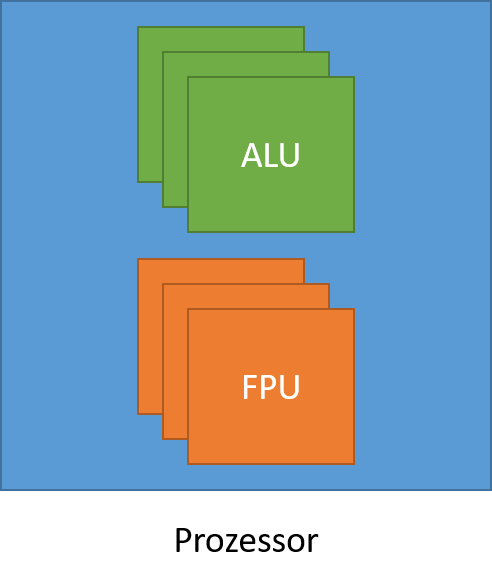
\includegraphics[width=4cm]{Abbildungen/Ebenen_der_Parallelitaet_Prozessor.png}
					\caption{Grafische Darstellung mehrerer Abarbeitungseinheiten innerhalb eines Prozessors.}
					\label{fig:EbenenDerParallelitaetProzessor}
				\end{figure}
			
			\subsubsection{Mehrere Abarbeitungseinheiten innerhalb eines Rechners}
				\label{MehrereAbarbeitungseinheitenRechner}
			
				Die nächst-größere Ebene stellt der Rechner selbst dar.\\
				Sind in einem Rechner mehrere Prozessoren bzw. CPU-Kerne verbaut, so kann auch in diesem Fall Parallelisierung stattfinden. Die Grafik \ref{fig:EbenenDerParallelitaetRechner} zeigt diese Situation grafisch. \cite{GrundlagenParallelisierungKegel}
				
				\begin{figure}
					\centering	
					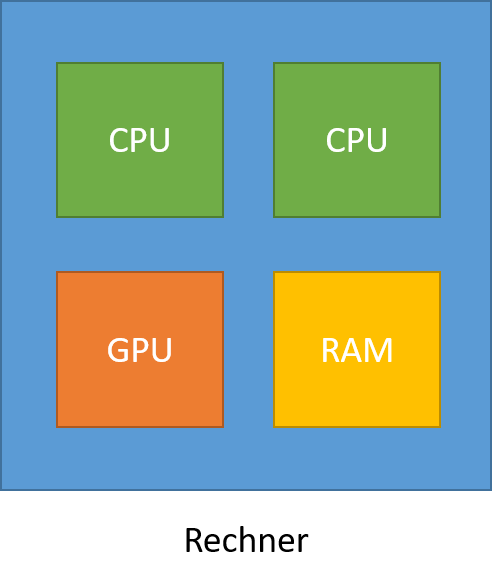
\includegraphics[width=4cm]{Abbildungen/Ebenen_der_Parallelitaet_Rechner.png}
					\caption{Grafische Darstellung mehrerer Abarbeitungseinheiten innerhalb eines Rechners.}
					\label{fig:EbenenDerParallelitaetRechner}
				\end{figure}
			
			\subsubsection{Mehrere Abarbeitungseinheiten innerhalb eines Clusters}
				\label{MehrereAbarbeitungseinheitenCluster}
			
				Werden nun mehrere Rechner verbunden (also vernetzt), so spricht man von einem \textit{Rechnerverbund} oder auch \textit{Rechnercluster}. \cite{RechnerverbundWikipedia}\\
				Da hierbei mehrere Rechner involviert sind, die jeweils unabhängig voneinander Aufgaben erledigen können, findet sich auch hier Parallelität.\\
				Die Grafik \ref{fig:EbenenDerParallelitaetCluster} soll diesen Umstand grafisch veranschaulichen. \cite{GrundlagenParallelisierungKegel}
				
				\begin{figure}
					\centering	
					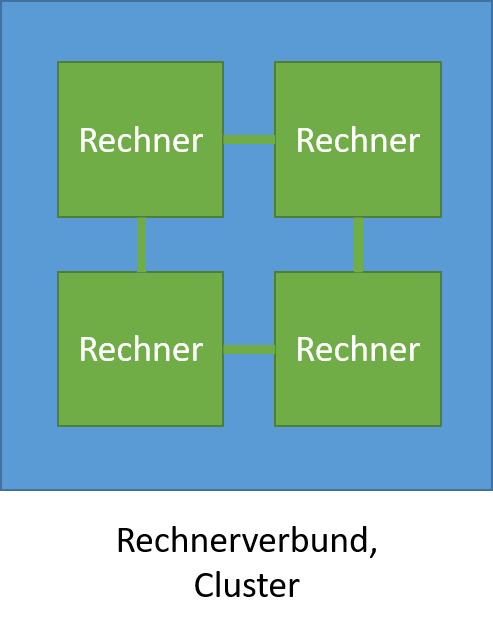
\includegraphics[width=4cm]{Abbildungen/Ebenen_der_Parallelitaet_Cluster.png}
					\caption{Grafische Darstellung mehrerer Abarbeitungseinheiten innerhalb eines Clusters.}
					\label{fig:EbenenDerParallelitaetCluster}
				\end{figure}
			
			\subsubsection{Mehrere Abarbeitungseinheiten innerhalb eines Grids}
				\label{MehrereAbarbeitungseinheitenGrid}
			
				Die höchste Ebene der Parallelität stellt ein \textit{Grid}, zu Deutsch \textit{Raster}, dar. In diesem Fall werden mehrere Rechner oder auch ganze Cluster zusammengeschlossen, also über ein Verbindungsnetzwerk verbunden. Auch in diesem Fall liegt also Parallelverarbeitung vor. Somit ist Grid-Computing eine Form des Hochleistungsrechnens, bei welcher ein virtueller Supercomputer kreiert wird. Damit werden meist sehr rechenintensive Probleme, wie beispielsweise in der Pharmaforschung und den Wirtschaftswissenschaften, gelöst. \cite{GridWikipedia}\\
				Die Abbildung \ref{fig:EbenenDerParallelitaetGrid} stellt dies in Form einer Grafik dar. Die Wolke steht dabei symbolisch für das Verbindungsnetzwerk. \cite{GrundlagenParallelisierungKegel}
				
				\begin{figure}
					\centering	
					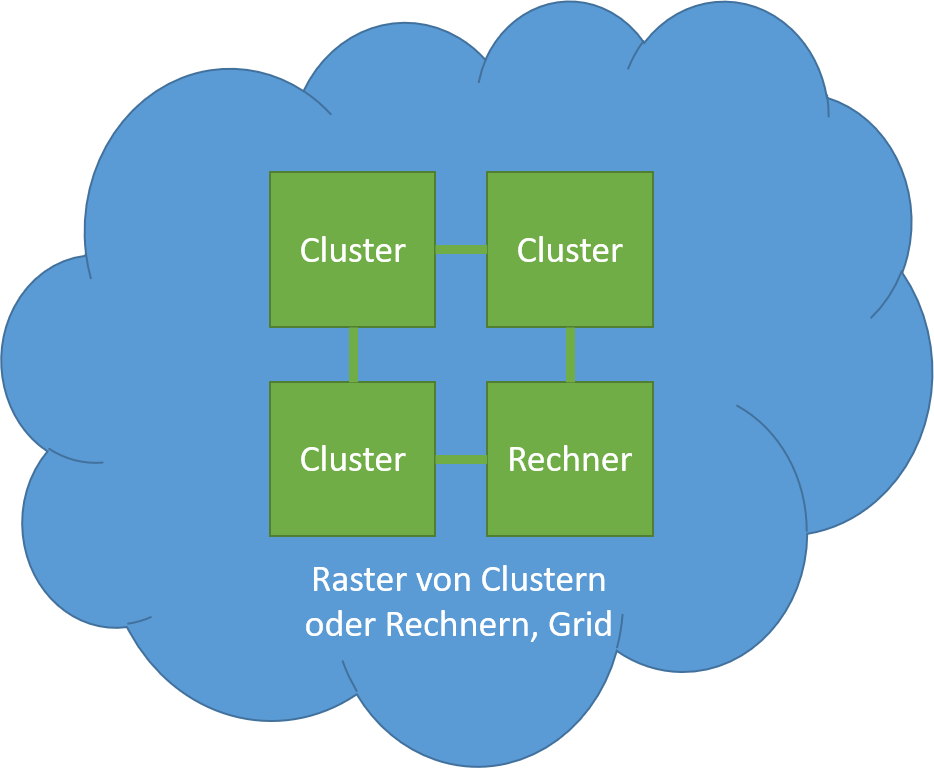
\includegraphics[width=5cm]{Abbildungen/Ebenen_der_Parallelitaet_Grid.png}
					\caption{Grafische Darstellung mehrerer Abarbeitungseinheiten innerhalb eines Grids.}
					\label{fig:EbenenDerParallelitaetGrid}
				\end{figure}
			
		\subsection{Arten und Einteilungen von Parallelrechnern}
		
			Es gibt verschiedene Ansätze, Parallelrechner zu klassifizieren. Eine bekannte Art ist die Klassifikation anhand der Art des Systems. Auch sehr verbreitet ist die Einteilung nach der Architektur nach Flynn\footnote{Michael J. Flynn (* 1934) ist ein US-amerikanischer Elektrotechniker. \cite{FlynnWikipedia}} und die Einteilung nach der Speicheranordnung. Auf diese drei Ansätze wird nun näher eingegangen.
			
			\subsubsection{Arten von Parallelrechnern}
				
				Die Arten von Parallelrechnern sind ein Einteilungskonzept, welches auf den in Kapitel \ref{EbenenParallelitaet} erläuterten Ebenen der Parallelität basiert.\\
				Nach diesem Schema existieren drei Arten von Parallelrechnern, welche im Folgenden genannt und erläutert werden. \cite{BSMultiprozessorsysteme}
				
				\begin{description}
					\item [Multikernprozessor-Systeme]
						Unter einem \textit{Multikernprozessor-System}, auch \textit{Mehrkernprozessor-System} genannt, versteht man einen Rechner, der über eine einzige CPU verfügt. Dieser Prozessor verfügt allerdings über mehrere Kerne, die auf einem Chip vereint sind. \cite{MehrkernprozessorWikipedia}\\
						Hier liegt also die unter Kapitel \ref{MehrereAbarbeitungseinheitenProzessor} eingeführte Ebene der Parallelität von mehreren Abarbeitungseinheiten innerhalb eines Prozessors vor.
					
					\item [Multiprozessor-Systeme]
						Ein \textit{Multiprozessor-System} oder \textit{Mehrprozessor-System} ist ein Rechner, der über mehr als einen Prozessor verfügt. \cite{MehrprozessorsystemWikipedia}\\
						In diesem Fall handelt es sich um die unter Kapitel \ref{MehrereAbarbeitungseinheitenRechner} eingeführte Ebene der Parallelverarbeitung von mehreren Abarbeitungseinheiten innerhalb eines Rechners.
					
					\item [Multicomputer-Systeme]
						Von einem \textit{Multicomputer-System} spricht man, wenn mehrere Rechner so über ein Kommunikationsnetzwerk verbunden werden, dass sie zusammen an einem gemeinsamen Problem arbeiten können. \cite{MulticomputerIGI}\\
						Somit liegen hier folglich die unter Kapitel \ref{MehrereAbarbeitungseinheitenCluster} bzw. \ref{MehrereAbarbeitungseinheitenGrid} eingeführten Ebenen der Parallelverarbeitung von mehreren Abarbeitungseinheiten innerhalb eines Clusters bzw. Grids vor.
				\end{description}
				
			\subsubsection{Einteilung der Architekturen nach der Flynnschen Klassifikation}
				
				Michael J. Flynn, ein US-amerikanischer Elektrotechniker \cite{FlynnWikipedia}, führte im Jahr 1966 eine Rechnerarchitektur-Einteilung ein, welche als \textit{Flynnsche Klassifikation} oder \textit{Flynnsche Taxonomie \footnote{Eine Taxonomie ist ein einheitliches Schema, mit dem Objekte nach bestimmten Kriterien in Kategorien eingeordnet werden. \cite{TaxonomieWikipedia}}} bezeichnet wird. Zunächst müssen für das Verständnis dieser Einteilung zwei Begriffe geklärt werden.
				
				\begin{description}
					\item [Befehlsstrom]
						Unter einem \textit{Befehlsstrom} versteht man Befehle, welche auf bestimmten Daten ausgeführt werden. Jeder Befehlsstrom muss dabei über einen eigenen Befehlszähler, der den nächsten auszuführenden Befehl des jeweiligen Befehlsstromes speichert, verfügen. \cite{FlynnsTaxonomie}
					\item [Datenstrom]
						Ein \textit{Datenstrom} ist eine Sequenz von Daten, auf denen Befehle ausgeführt werden können. \cite{FlynnsTaxonomie}
				\end{description}
			
				Auf Grund der Anzahl der vorhandenen Befehls- und Datenströme unterscheidet Flynn vier verschiedenen Kategorien, welche in der Übersichtstabelle \ref{tab:UebersichtFlynnscheKlassifikation} aufgeführt sind.
				
				\begin{table}
					\caption{Übersicht zur Flynnschen Klassifikation.}
					\begin{tabular}{c|c|c}
						& Single Instruction & Multiple Instruction \\
						\hline
						Single Data & SISD & MISD \\
						Multiple Data & SIMD & MIMD \\
					\end{tabular}
					\label{tab:UebersichtFlynnscheKlassifikation}
				\end{table}
			
				Diese vier Kategorien werden im Folgenden näher erläutert.
			
				\begin{description}
					
					\item [Single Instruction, Single Data (SISD)]
					
						Ein SISD-System verfügt nur über eine Ausführungseinheit, welche Zugriff auf einen einzigen Programm- und Daten-Speicher besitzt. In jedem Schritt lädt die Ausführungseinheit einen Befehl und ein Daten-Element, führt den Befehl auf dem Element aus und schreibt das Ergebnis in den Speicher zurück.\\
						Somit ist ein solches System ein gewöhnlicher, sequentiell arbeitender Rechner, welcher nach dem Von-Neumann-Modell arbeitet, also ein Einprozessorsystem. Auf dieser Art von Computer kann man Parallelität folglich nur als Quasiparallelität realisieren. \cite{ParaProgRauber} \cite{FlynnscheKlassifikationWikipedia} \cite{EntwicklungParallelerProgramme}
						
					\item [Multiple Instruction, Single Data (MISD)]
					
						Ein MISD-System besteht aus mehreren Ausführungseinheiten, wobei jede Einheit einen eigenen Programm-Speicher besitzt. Alle Einheiten teilen sich allerdings einen Daten-Speicher. In jedem Schritt erhält jede Ausführungseinheit \textit{das selbe} Daten-Element aus dem Daten-Speicher. Jede Einheit lädt allerdings den auszuführenden Befehl aus seinem privaten Programm-Speicher. Das führt dazu, dass die jeweiligen Ausführungseinheiten parallel verschiedene Befehle auf den gleichen Daten ausführen.\\
						Ein solches paralleles System wurde noch nie für den kommerziellen Gebrauch gefertigt, da hier mehrere Prozessoren gleichzeitig auf den selben Daten Befehle ausführen, weshalb sich die Frage der Sinnhaftigkeit eines solchen Systemes stellt. \cite{ParaProgRauber} \cite{FlynnscheKlassifikationWikipedia} \cite{EntwicklungParallelerProgramme}
					
					\item [Single Instruction, Multiple Data (SIMD)]
					
						In einem SIMD-System sind mehrere Ausführungseinheiten verbaut, wobei jede Einheit Zugriff auf einen privaten Daten-Speicher besitzt. Allerdings teilen sich in diesem Fall alle Einheiten den selben Programm-Speicher, wobei eine eigens dafür konstruierte Steuerungseinheit Befehle lädt und an die Ausführungseinheiten weitergibt, was bedeutet, dass alle Einheiten das selbe Programm und damit die selben Befehle ausführen. In jedem Schritt erhalten alle Ausführungseinheiten von der Steuereinheit den selben Befehl, laden allerdings verschiedene Daten-Elemente aus ihrem eigenen Daten-Speicher, auf welchen der Befehl dann ausgeführt wird.\\
						Aus diesem Grund wird der selbe Befehl \textit{parallel und synchron} von allen Einheiten auf verschiedenen Daten-Elementen ausgeführt.\\
						Der SIMD-Ansatz kann sehr effizient sein und wird beispielsweise bei Computer-Grafik-Algorithmen, wo die selben Befehle auf vielen Daten ausgeführt werden müssen, verwendet. Die in Kapitel \ref{Vektorrechner} erläuterten Vektorrechner lassen sich der SIMD-Klasse zuordnen. \cite{ParaProgRauber} \cite{FlynnscheKlassifikationWikipedia} \cite{EntwicklungParallelerProgramme}
						
					\item [Multiple Instruction, Multiple Data (MIMD)]
					
						Ein MIMD-System verfügt über mehrere Ausführungseinheiten, welche alle Zugriff auf einen eigenen Programm- und Daten-Speicher besitzen. In jedem Schritt lädt jede Einheit einen eigenen Befehl und ein eigenes Daten-Element, führt den Befehl auf dem Element aus und schreibt das Ergebnis in den eigenen Daten-Speicher zurück.\\
						Aus diesem Grund führen jeweils die einzelnen Ausführungseinheiten einen eigenen Befehl \textit{parallel und asynchron} auf verschiedenen Daten-Elementen aus.\\
						Beispiele für Systeme, die der MIMD-Klasse zugeordnet werden können, sind Multikernprozessor- oder auch Cluster-Systeme. \cite{ParaProgRauber} \cite{FlynnscheKlassifikationWikipedia} \cite{EntwicklungParallelerProgramme}
						
				\end{description}
			
				SIMD-Systeme sind im Gegensatz zu MIMD-Systemen einfach zu programmieren, weil nur ein Programmfluss existiert, dem alle Prozessoren synchron folgen. Somit ist kein Synchronisation auf Programm-Ebene nötig. Allerdings stellt die synchrone Ausführung auch eine Einschränkung dar, da die Daten-Elemente sich unterscheiden können. Bedingungen der folgenden Form müssen aus diesem Grund in zwei getrennten Schritten ausgeführt werden.
				
				\lstinputlisting[language=C, breaklines=true]{Quellcode/if-Statement_SIMD-Systeme.c}
				
				Im ersten Schritt müssen alle Ausführungseinheiten, deren lokale Variable \textit{b} gleich 0 ist, den \textit{then}-Block der \textit{if}-Anweisung ausführen. Im zweiten Schritt müssen alle anderen Ausführungseinheiten, bei welchen dies folglich nicht zutrifft und \textit{b} ungleich 0 ist, den \textit{else}-Block ausführen.\\
				Somit wird klar, dass MIMD-Rechner flexibler sind als SIMD-Systeme, da jede Ausführungseinheit über einen eigenen Programmfluss verfügt.\\
				Zusammenfassend lässt sich zur Flynnschen Klassifikation aussagen, dass sie zwar nur eine grobe Einteilung vornimmt, welche allerdings einen Überblick über die Arbeitsweise eines Parallelrechners gibt. \cite{ParaProgRauber}
		
			\subsubsection{Einteilung von Parallelrechnern nach der Art der Speicheranordnung}
			
				Teilt man die Parallelrechner nach der Art der Speicheranordnung ein, so erhält man zwei Klassen von Parallelrechnern, welche im Folgenden erläutert werden.
				
				\begin{description}
					\item [Parallelrechner mit verteiltem Speicher]
						Rechner mit verteiltem Speicher, auch \textit{Distributed Memory} genannt, bestehen aus \textit{n} Prozessoren $P_1, P_2, P_3, ... P_i$, wobei jedem Prozessor genau ein privater lokaler Speicher $M_i$ zugeteilt ist. Nur der Prozessor $P_i$ darf auf den Speicher $M_i$ zugreifen. Umgekehrt gilt das selbe: Ein Prozessor $P_i$ darf nur auf den Speicher $M_i$ zugreifen.\\
						Die einzelnen Rechner (mit Prozessor, Hauptspeicher und eventuell weiteren Ressourcen) werden über ein Verbindungsnetzwerk zu einem Parallelrechner verbunden. Die Kommunikation läuft dabei anhand des sogenannten \textit{Message Passings} (Nachrichtenaustausch) ab, das bedeutet, dass die Rechner untereinander Nachrichten austauschen. Das Konzept des \textit{Message Passings} wird unter Kapitel \ref{MPI} genauer erläutert.\\
						Die Abbildung \ref{fig:ParallelrechnerVerteilterSpeicher} soll dieses Konzept nochmals bildlich veranschaulichen. \cite{EntwicklungParallelerProgramme}
						
					\item[Parallelrechner mit gemeinsamem Speicher]
						Ein anderer Ansatz ist das Konzept des gemeinsamen Speichers, welches auch als \textit{Shared Memory} bezeichnet wird. Dabei existieren auch \textit{n} Prozessoren $P_1, P_2, P_3, ... P_i$, allerdings ist allen Prozessoren ein- und derselbe gemeinsame (Haupt-)Speicher zugeteilt. Durch diesen gemeinsamen Datenspeicher und den damit verbundenen gemeinsamen Variablen erfolgt auch die Kommunikation zwischen den einzelnen Prozessoren.\\
						Die Abbildung \ref{fig:ParallelrechnerGemeinsamerSpeicher} erläutert dieses Prinzip auch auf grafischer Ebene.\\
						Es gibt zwei Modelle, nach denen \textit{Shared Memory}-Systeme auf den Speicher zugreifen. Auch diese werden im Folgenden näher beleuchtet. \cite{EntwicklungParallelerProgramme}
						
						\begin{description}
							\item [Uniform Memory Access (UMA)]
								Bei diesem Modell sind alle Prozessoren beim Zugriff auf den Speicher gleichberechtigt, insbesondere die Zugriffszeiten sind für alle CPUs gleich. Somit besteht beim Zugriff auf Ressourcen kein Unterschied zwischen den einzelnen Ausführungseinheiten.\\
								Sogenannte \textit{Symmetrische Multiprozessoren} (SMP) sind UMA-Systeme. \cite{EntwicklungParallelerProgramme}
								
							\item [Non-Uniform Memory Access (NUMA)]
								Im Rahmen dieses Modells können auch alle Prozessoren auf den gemeinsamen Speicher zugreifen. Allerdings variieren in die Fall die Zugriffszeiten je nach Ort, an dem sich die angesprochene Speicheradresse befindet. Der Grund dafür ist, dass der Speicher auf mehrere Knoten verteilt ist. Somit ist der Zugriff auf einen lokalen Speicherknoten schneller als auf entfernte. Für den Programmierer besteht allerdings kaum bis gar kein Unterschied zu UMA-Systemen. \cite{EntwicklungParallelerProgramme}
						\end{description}
				\end{description}
			
				\begin{figure}
					\centering	
					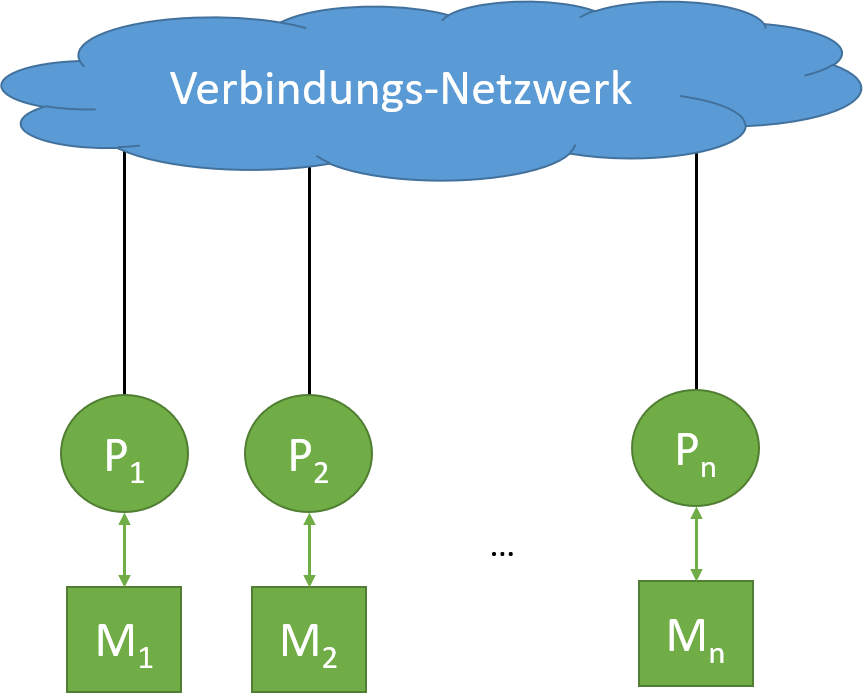
\includegraphics[width=7cm]{Abbildungen/Parallelrechner_mit_verteiltem_Speicher.png}
					\caption{Grafische Darstellung eines Parallelrechners mit verteiltem Speicher.}
					\label{fig:ParallelrechnerVerteilterSpeicher}
				\end{figure}
			
				\begin{figure}
					\centering	
					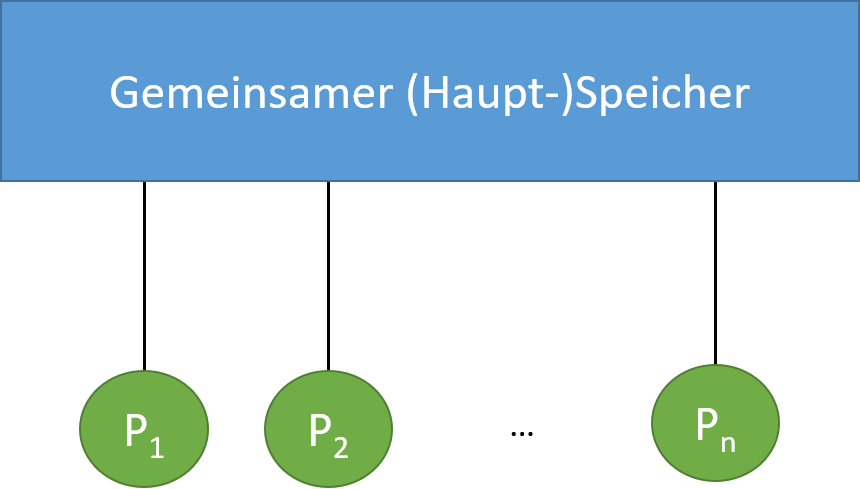
\includegraphics[width=7cm]{Abbildungen/Parallelrechner_mit_gemeinsamem_Speicher.png}
					\caption{Grafische Darstellung eines Parallelrechners mit gemeinsamem Speicher.}
					\label{fig:ParallelrechnerGemeinsamerSpeicher}
				\end{figure}
			
				Die Programmierung gestaltet sich bei Rechnern mit gemeinsamem Speicher meist einfacher als bei verteiltem Speicher, da alle Prozessoren Zugriff auf den Speicher besitzen und somit der Programmierer nicht explizit für die Steuerung des Versendens und Empfangens von Informationen zuständig ist. Allerdings kann es durch die gemeinsame Ressource zu Problemen kommen, die beispielsweise durch die unter Kapitel \ref{ProzessSynchronisation} erklärten Mechanismen gelöst werden können.\\
				Zu solchen Problemen kommt es in der Regel bei der Verwendung eines Rechners mit verteiltem Speicher nicht, da der Großteil des Datenflusses hierbei meist nur zwischen dem Prozessor und dessen lokalem Speicher abläuft. Doch das Umgehen der Synchronisierungsproblematik führt zu einer anderen Schwierigkeit: Werden Daten von anderen Prozessoren benötigt, so muss der Austausch von Informationen anhand von speziellen Befehlen erfolgen, welche die Informationen dann über ein Netzwerk vermitteln. \cite{ParalleleNumerischeVerfahren}\\
				Anzumerken ist noch, dass es auch hybride Systeme gibt, welche als \textit{Hybrid Distributed-Shared Memory}-Systeme bezeichnet werden. Diese Rechner verwenden eine Mischung aus gemeinsamem und verteiltem Speicher. Dabei handelt es sich um Systeme, welche aus mehreren Rechnern mit gemeinsamem Speicher bestehen. Die Prozessoren, die jeweils zu einem Parallelrechner mit gemeinsamem Speicher gehören, können alle auf den selben globalen Speicher zugreifen. Der verteilte Speicher kommt durch den Zusammenschluss mehrere Shared-Memory-Systeme zustande. Aus diesem Grund ist eine Netzwerk-Kommunikation von Nöten, um Informationen zwischen diesen Teilsystemen auszutauschen. \cite{EntwicklungParallelerProgramme}
				
	\section{Metriken und Modelle zur Performance-Analyse und -Vorhersage paralleler Programme}
		
		Die Bewertung der Güte von Programmen ist eine grundlegende Voraussetzung, wenn man effiziente Programme erstellen möchte. Da es bei der parallelen Programmierung nahezu ausschließlich um das Erzielen einer Performance-Verbesserung geht, spielt hier die Analyse und die Optimierung der Abläufe innerhalb eines Programmes eine zentrale Rolle. Aus diesem Grund wurden einige Kenngrößen und Modelle entwickelt, die die Performance-Analyse und -Vorhersage von Programmen mit Parallelverarbeitung ermöglichen.\\
		Die Größe, welche es in diesem Zusammenhang vor allem zu analysieren und wenn möglich reduzieren gilt, ist die \textit{Ausführungszeit} des Programmes, auch \textit{Laufzeit} genannt. Der Benutzer eines Rechner-Systems ist an sehr kurzen Antwort- bzw. Reaktionszeiten interessiert, was wiederum auf die Zeit zwischen dem Start und der Terminierung eines Programmes, also die Ausführungszeit, führt.\\
		Auf der anderen Seite zielen Rechenzentren, welche extrem komplexe Berechnungen mittels Supercomputer zu lösen versuchen, auf einen hohen \textit{Durchsatz} ab, wobei dieser Durchsatz die durchschnittliche Anzahl an Arbeitseinheiten, welche pro Zeiteinheit verrichtet werden können, darstellt. \cite{ParaProgRauber}
		
		\subsection{Kosten, Speedup und Effizienz}
		
			Die Laufzeit eines parallelen Programmes auf einer speziellen Ausführungsplattform ist ein wichtiges Kriterium zur Bewertung des Programmes.\\
			Die \textit{parallele Laufzeit} $t_P(n)$ eines Programmes ist dabei die Zeit zwischen dem Starten des Programmes auf dem ersten Prozessor und dem Ende der Ausführung auf dem letzten beteiligten Prozessor. Dabei steht $t$ für die Laufzeit, $P$ für die Anzahl an beteiligten, parallel arbeitenden Prozessoren und $n$ für die Größe des zu lösenden Problems. Diese sogenannte \textit{Problemgröße} hängt im einfachsten Fall von den Eingabe-Daten ab. Ein Beispiel hierfür ist die Anzahl von Gleichungen, welche von einer Software gelöst werden muss.\\
			Des Weiteren ist auch $t_S(n)$ von Bedeutung. Dies ist die Laufzeit des schnellsten sequentiellen Programmes, das das gegebene Problem der Größe $n$ löst.\\
			Aus diesen Kennzahlen lassen sich einige weitere Kenngrößen ableiten, welche im Folgenden erläutert werden sollen. \cite{ParaProgRauber}
			
			\subsubsection{Kosten eines parallelen Programmes}
			
				Die \textit{Kosten} $C_P(n)$ eines parallelen Programmes mit der Problemgröße $n$, wobei $P$ Prozessoren an der Ausführung beteiligt sind, sind wie folgt definiert:
				
				\[ C_P(n) = P \cdot t_P(n) \]
				
				Die daraus resultierende Zahl gibt also an, wie viel Arbeit alle Prozessoren zusammen verrichtet haben. Dabei wird davon ausgegangen, dass das Programm vollkommen parallel abläuft und die Last auf alle Prozessen genau im gleichen Maße verteilt wird.\\
				Ein solches Programm wird \textit{kosten-optimal} genannt, falls $C_P(n) = t_S(n)$ gilt. Das bedeutet, dass das kosten-optimale parallele Programm exakt gleich viele Operationen wie das schnellste sequentielle Programm ausführt. Ist dies der Fall, so würde durch die parallele Ausführung an sich \textbf{kein} zusätzlicher Aufwand, z.B. für Kommunikation oder Synchronisation, entstehen. \cite{ParaProgRauber}
				
			\subsubsection{Speedup eines parallelen Programmes}
				\label{Speedup}
			
				Der \textit{Speedup} $S_P(n)$, auch \textit{Geschwindigkeitsgewinn} oder \textit{Beschleunigung} genannt, ist die wohl simpelste und aussagekräftigste Kennzahl.\\
				Er lässt sich durch die folgende Formel ausdrücken:
				
				\[ S_P(n) = \frac{t_S(n)}{t_P(n)} \]
				
				Aus dem obigen Ausdruck wird klar, dass der Speedup die Laufzeit des besten sequentiellen Programmes mit der Laufzeit des parallelen Programmes unter Verwendung von $P$ Prozessoren vergleicht, wobei beide Programme das selbe Problem lösen müssen. Somit wird der Vorteil, welcher sich aus der Parallelisierung ergibt, klar. Er gibt also an, dass das parallele Programm, welches $P$ Prozessoren verwendet, $S_P(n)$-mal schneller in der Ausführung als die sequentielle Lösung ist.\\
				Den Idealfall bildet ein Speedup von $P$, da dies bedeuten würde, dass der Einsatz von $P$ Prozessoren zu einer $P$-fachen Beschleunigung führen würde. Folglich gilt für den Speedup in der Theorie immer der folgende Zusammenhang:
				
				\[ S_P(n) \leq P \]
				
				Im Fall von \(S_P(n) = P\) spricht man von einem \textit{linearen} Speedup. Dies ist in der Theorie der Optimalfall.\\
				
				Falls \(S_P(n) \geq P\) gilt, so ist der sequentielle Algorithmus nicht der beste sequentielle Algorithmus zur Lösung des gegebenen Problems, da die Ausführung des parallelen Programmes auf nur einem Prozessor unter Verwendung von einem Scheduling-Algorithmus wie beispielsweise Round-Robin, welcher in Kapitel \ref{ProzessScheduling} erklärt wurde, zu einer besseren Laufzeit führen würde. Aus dieser sequentiell abgearbeiteten Version des parallelen Algorithmus kann dann ein neuer sequentieller Algorithmus konstruiert werden, sodass \(S_P(n) \geq P\) nicht mehr gilt.\\
				Die Berechnung des Speedups schließt wie bereits erwähnt den Vergleich mit dem schnellsten sequentiellen Algorithmus mit ein. Dieser Algorithmus kann in einigen Fällen allerdings schwierig zu finden bzw. zu erstellen sein.\\
				Aus diesem Grund wird für die Berechnung des Speedups in der Praxis oft nicht die Laufzeit des besten sequentiellen Algorithmuses verwendet, sondern diejenige des parallelen Algorithmuses unter Verwendung von nur einem Prozessor, also $t_1(n)$.
				Unter diesen Umständen ergibt sich der Speedup durch die folgende Formel:
				
				\[ S_P(n) = \frac{t_1(n)}{t_P(n)} \]
				
				In der Praxis ist \(S_P(n) \geq P\) allerdings trotzdem möglich, in diesem Fall spricht man von einem \textit{superlinearen} Speedup. Dieser Effekt kann durch die Caches der Prozessoren auftreten. Dies ist darin begründet, dass jeder Prozessor auch einen zusätzlichen Cache beinhaltet. Wird der Algorithmus auf einem Prozessor ausgeführt, so ist es durchaus möglich, dass die vom Prozessor zu verarbeitenden Daten nicht vollständig im Cache des Prozessors Platz haben, was zu sogenannten Cache-Misses\footnote{Ein Cache-Miss tritt auf, wenn von einem Programm angeforderte Daten nicht im Cache gefunden werden können. Dies führt zu einer Ausführungsverzögerung, da das Programm dann auf anderen Speicher-Ebenen (in Caches höheren Levels oder auch im Hauptspeicher) nach den Daten suchen muss. \cite{CacheMissTechopedia}} während der Ausführung führt, welche die Ausführung verzögern und die Laufzeit verlängern. Wird das Programm jedoch auf mehreren Prozessoren parallel ausgeführt, so könnte es passieren, dass durch den zusätzlichen Cache-Speicher, der mit den hinzugekommenen Prozessoren einhergeht, nun genügend Speicher vorhanden sein könnte, sodass es zu keinen (oder weniger) Cache-Misses käme, was zu einem superlinearen Speedup führen könnte.\\
				Doch ein solcher superlinearer Speedup tritt in der Praxis nur äußerst selten auf. Meist wird auf Grund des mit der Parallelisierung einhergehenden Mehraufwandes kein linearer, geschweige denn ein superlinearer Speedup erreicht. \cite{ParaProgRauber}

			\subsubsection{Effizienz eines parallelen Programmes}
			
				Eine Metrik, welche auf dem unter Kapitel \ref{Speedup} erläuterten Konzept des Speedups aufbaut, ist die sogenannte \textit{Effizienz}. Sie ist durch die folgende Formel gegeben.
				
				\[ E_P(n) = \frac{S_P(n)}{P} \]
				
				Durch das Ausdrücken des Speedups $S_P(n)$ als \( \frac{t_S(n)}{t_P(n)} \) lässt sich die Effizienz auch wie folgt ausdrücken:
				
				\[ E_P(n) = \frac{\frac{t_S(n)}{t_P(n)}}{P} = \frac{t_S(n)}{P \cdot t_P(n)} = \frac{t_S(n)}{C_P(n)} \]
				
				Die Effizienz gibt an, wie effizient die einzelnen Prozessoren genutzt werden und an der Berechnung mitwirken. Sie ließe sich folglich auch einfach durch Multiplikation mit 100 in Prozent angeben. Diese Zahl würde dann der Auslastung der einzelnen Prozessoren entsprechen.\\
				Falls es zu keinem superlinearen Speedup kommt, gilt stets \( 0 \leq E_P(n) \leq 1 \).\\
				Ein idealer, linearer Speedup $S_P(n) = P$ entspricht einer Effizienz von $E_P(n) = 1 = 100\%$.\\
				Die Effizienz gibt folglich auch darüber Auskunft, wie nahe die Beschleunigung, welche durch die Parallelisierung erreicht wird, an der idealen Beschleunigung liegt. Eine Effizienz von 100\% entspricht dabei dem Ideal, da ein Einsatz von $P$ Prozessoren in diesem Fall eine $P$-fache Beschleunigung mit sich bringen würde. \cite{ParaProgRauber}
			
		\subsection{Mathematische Gesetze und Modelle}
			
			Um Aussagen über den Nutzen der Parallelisierung im Allgemeinen zu treffen, wurden verschiedenste mathematische Modelle entwickelt, welche die Parallelisierung teilweise aus vollkommen verschiedenen Blickwinkeln aus betrachten.\\
			Im Folgenden wird auf die beiden wichtigsten Gesetze, nämlich das \textit{Amdahlsche Gesetz} und das \textit{Gustafsonsche Gesetz} eingegangen.
			
			\subsubsection{Das Amdahlsche Gesetz}
			
				Dieses Gesetz, welches 1967 von Gene Amdahl\footnote{Gene Myron Amdahl (1922 - 2015) war ein US-amerikanischer Computerarchitekt und Hi-Tech-Unternehmer norwegischer Abstammung. \cite{GeneAmdahlWikipedia}} veröffentlicht wurde, beschäftigt sich mit der Beschleunigung von Programmen durch eine parallele Ausführung. Amdahl stellte sich die Frage, wie weit diese Beschleunigung getrieben werden kann.\\
				Dieses Gesetz geht davon aus, dass ein Programm im Wesentlichen aus nur zwei Teilen besteht: Einem sequentiellen Anteil, der nicht parallelisierbar ist, und einem parallelen Anteil, der durch Parallelisierung \textit{beliebig} beschleunigt werden kann.\\
				Amdahl nimmt an, dass das Programm zunächst auf einem Ein-Prozessor-System gestartet wird und normiert die hierbei gemessene Laufzeit auf 1. Den parallelisierbaren Anteil der Laufzeit nennt man $t_{Par}$, den sequentiellen Anteil folglich $1 - t_{Par}$.\\
				Auf einem System mit $P$ Prozessoren verhält sich das Programm nun anders: Der sequentielle Anteil $1 - t_{Par}$ ändert sich nicht, der parallele Anteil $t_{Par}$ wird im Optimalfall auf alle Prozessoren gleichermaßen aufgeteilt und wird $P$-mal schneller ausgeführt, weshalb aus $t_{Par}$ der Term $\frac{t_{Par}}{P}$ wird. Die Laufzeit $t_{Ges}(P)$ auf einem $P$-Prozessor-System lässt sich also durch den folgenden Term angeben.
				
				\[ t_{Ges}(P) = (1 - t_{Par}) + \frac{t_{Par}}{P} \]
			
				Aus dem obigen Term wird auch schnell wieder klar, dass für $P = 1$, also auf einem Ein-Prozessor-System, die gesamte Laufzeit $t_{Ges}(1)$ genau 1 ist.\\
				Der Geschwindigkeitsgewinn, also der Speedup, lässt sich nun sehr einfach errechnen. Dabei wird in der folgenden Betrachtung die Problemgröße $n$ vernachlässigt, um den Grundgedanken Amdahls besser folgen zu können.
				
				\[ S_P = \frac{t_{Ges}(1)}{t_{Ges}(P)} = \frac{1}{(1 - t_{Par}) + \frac{t_{Par}}{P}} \]
			
				Der obige Term entspricht bereits dem Amdahlschen Gesetz.\\
				Eine wichtige und oft zitierte Konsequenz aus dem obigen Gesetz ist eine Aussage über die maximale Beschleunigung, die mittels Parallelisierung erzielt werden kann. Bildet man den Grenzwert des obigen Speedups für beliebig viele Prozessoren, so kommt man zur folgenden Rechnung.
				
				\[ \lim\limits_{P \to \infty} S_P = \lim\limits_{P \to \infty} \frac{1}{(1 - t_{Par}) + \frac{t_{Par}}{P}} = \frac{1}{(1 - t_{Par}) + 0} = \frac{1}{1 - t_{Par}} \]
			
				Aus dem obigen Zusammenhang wird klar, dass ein Programm durch Parallelisierung \textit{nicht beliebig} beschleunigt werden kann, sondern bestimmte Grenzen existieren. Für den Speedup gilt laut Amdahl also die folgende Ungleichung:
				
				\[ S_P < \frac{1}{1 - t_{Par}} \]
				
				Im Nenner des obigen Bruches steht genau die sequentielle Laufzeit $1 - t_{Par}$, welche durch Parallelisierung nicht beeinflusst werden kann. Dieses Gesetz sagt also aus, dass die Verwendung von mehr Prozessoren nicht immer einen Mehrwert mit sich bringt, sondern eine Grenze für den Speedup existiert, der sich der Speedup bei Verwendung von beliebig vielen Prozessoren annähert.\\
				Dieses Modell führte zu viel Pessimismus in Bezug auf massive Parallelisierung, da sich beispielsweise ein zu 90\% parallelisierbares Programm mit $t_{Par} = 0,9$ auch bei Verwendung von beliebig vielen Prozessoren nur um den Faktor 10 ($\frac{1}{1 - t_{Par}} = \frac{1}{1 - 0,9} = 10$) beschleunigen lässt.\\
				Das in Abbildung \ref{fig:Amdahlsches_Gesetz} dargestellte Diagramm zeigt den Zusammenhang zwischen dem Speedup und der Anzahl der verwendeten Prozessoren für verschieden gut parallelisierbare Programme. Die Prozessor-Achse P ist dabei logarithmisch eingeteilt, dass bedeutet, dass sich die Anzahl der verwendeten Prozessoren bei jedem Schritt verdoppelt.
				
				\begin{figure}
					\centering	
					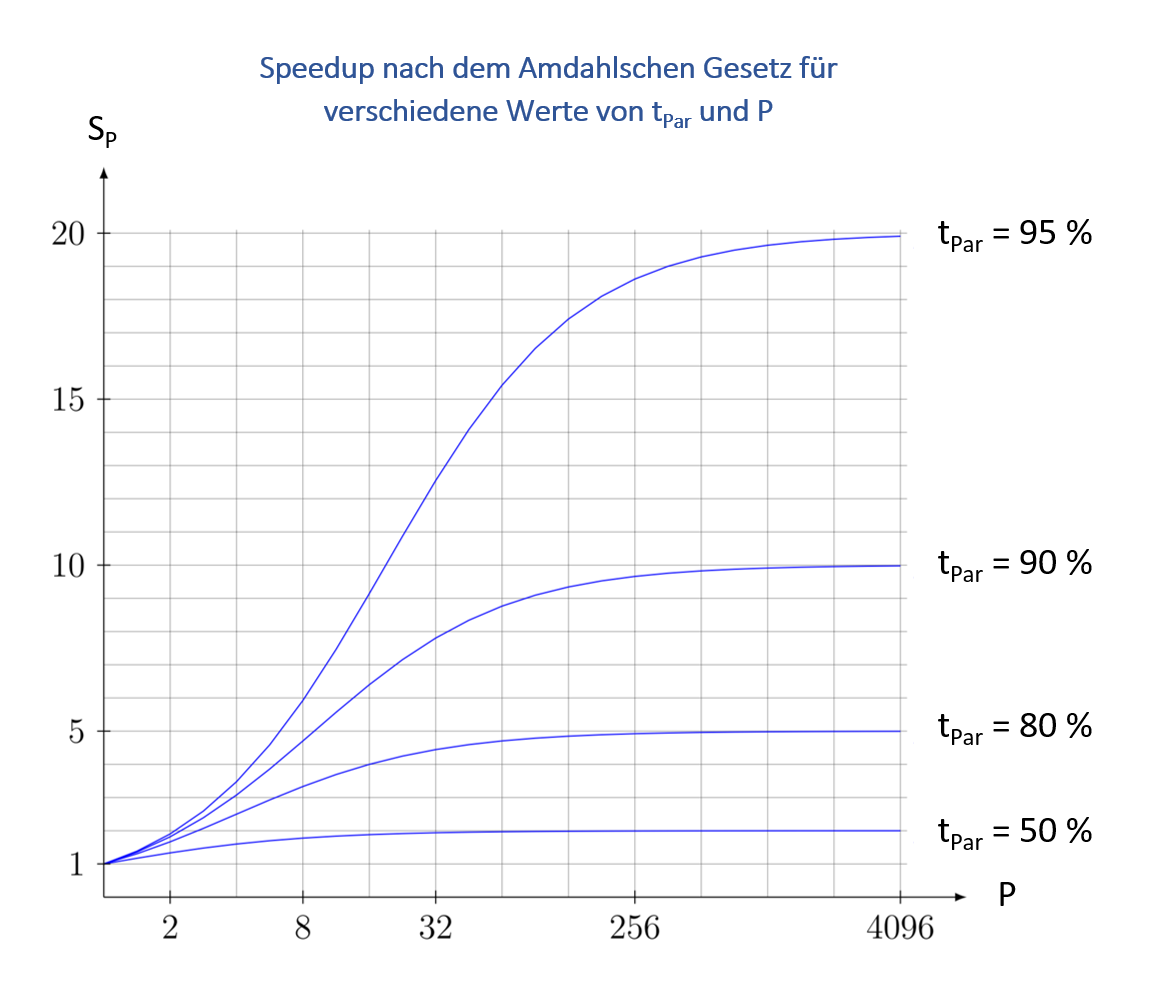
\includegraphics[width=9cm]{Abbildungen/Amdahlsches_Gesetz.png}
					\caption{Grafische Darstellung des Zusammenhangs zwischen dem aus dem Amdahlschen Gesetz ableitbaren Speedup und der Anzahl der verwendeten Prozessoren für verschieden gut parallelisierbare Programme. \cite{GesetzeParallelierung}}
					\label{fig:Amdahlsches_Gesetz}
				\end{figure}
				
				Eine weitere Folge aus diesem Modell ist das Gesetz des abnehmenden Gewinns. Wenn bereits viele Prozessoren verwendet werden, so wirkt sich die Hinzunahme eines weiteren Prozessors nur mehr geringfügig auf die gesamte Laufzeit des Programmes aus.\\
				
				Aus den bereits bekannten Gründen führte dieses Modell in der Vergangenheit zu einer negativen Einstellung in Bezug auf die Parallelisierung. Dabei sei allerdings darauf hingewiesen, dass dieses Gesetz nur ein Modell ist und deshalb bestimmten Grenzen unterworfen ist.\\
				Die folgenden Sachverhalte werden vom Amdahlschen Gesetz nicht beachtet:
				
				\begin{itemize}
					\item Umso mehr Prozessoren an einem Problem gemeinsam arbeiten, umso größer wird auch der Kommunikationsaufwand, welcher den zu erwartenden Speedup nochmals senkt.
					\item Mit einem dazukommenden Prozessor gehen auch andere zusätzliche Ressourcen einher. Beispielsweise ist jeder zusätzliche Prozessor mit einem eigenen Cache ausgestattet, weshalb für die Berechnungen insgesamt mehr Cache zur Verfügung steht. Es kann auch dazu kommen, dass ein Problem, dass auf einem Ein-Prozessor-System nicht auf ein Mal im Speicher Platz hatte, durch die Parallelisierung in Teilprobleme zerlegt werden kann, sodass diese in den Caches der beteiligten Prozessoren Platz haben. In diesem Fall können die Teilprobleme und damit auch das gesamte Problem in einer viel schnelleren Zeit gelöst werden.
					\item Manchmal ist es gar nicht das höchste Ziel, ein Problem in beliebig kleiner Zeit zu lösen, sondern ein beliebig großes Problem in immer der selben Zeit zu lösen. Dieser Ansatz führt zum Gustafsonschen Gesetz, welches unter Kapitel \ref{GustafsonschesGesetz} behandelt wird. \cite{AmdahlschesGesetzWikipedia} \cite{GesetzeParallelierung}
				\end{itemize}

			\subsubsection{Das Gustafsonsche Gesetz (Gesetz von Gustafson-Barsis)}
				\label{GustafsonschesGesetz}
				
				Um dem Pessimismus, der sich aus dem Amdahlschen Gesetz ergibt, entgegenzuwirken, schuf John Gustafson\footnote{John Leroy Gustafson (* 1955) ist ein amerikanischer Informatiker und Geschäftsmann.\cite{JohnGustafsonWikipedia}} im Jahre 1988 ein eigenes Gesetz, in welchem er die Parallelisierung von einem anderen Standpunkt aus betrachtete und somit zeigte, dass sich massive Parallelisierung trotzdem lohnen kann. Nach seinem Gustafsonschen Gesetz (auch bekannt als Gesetz von Gustafson-Barsis) kann man ein Problem zwar nicht in beliebig kleiner Zeit lösen, aber in einer bestimmten Zeit beliebig große Probleme berechnen.\\
				Eine grundlegende Säule dieses Modells ist die Einbeziehung der Problemgröße $n$, welche von Amdahl vernachlässigt wurde. Die Problemgröße kann man sich im einfachsten Fall als die Größe der Eingabedaten des Programmes vorstellen. Das ursprünglich zu lösende Problem hat in diesem Fall die Problemgröße $n = 1$. Die Laufzeit dieses Programmes auf einem Ein-Prozessor-System wird wiederum auf 1 normiert. Der parallele Anteil des Programmes hat auf diesem System einen Anteil von $t'_{Par}$.\\
				Nun hat sich Gustafson Gedanken darüber gemacht, wie sich die Laufzeit verändert, wenn die Problemgröße $n$ erhöht wird. Er argumentiert dabei, dass sich diese Erhöhung nur auf den parallelen Anteil der Laufzeit auswirkt, da hierbei oft beispielsweise Vektor-Operationen berechnet werden, deren Dimension direkt von der Größe der Eingabedaten abhängt. Der sequentielle Anteil besteht in diesem Modell hingegen vor allem aus Initialisierungsvorgängen, auf welche die Problemgröße keinen Einfluss ausübt. Dies führt im Allgemeinen zur folgenden Laufzeit $t_{Ges}(P, n)$, wobei hier $P = 1$ gilt.
				
				\[ t_{Ges}(1, n) = (1 - t'_{Par}) + n \cdot t'_{Par} \]
				
				Analog zum Amdahlschen Gesetz stellte sich nun auch Gustafon die Frage, wie sich der Einsatz von $P$-Prozessor-Systemen auf die gesamte Laufzeit $t_{Ges}(P, n)$ auswirkt. In diesem Fall bleibt auch hier der sequentielle Anteil unverändert, während der parallele Anteil im Optimalfall wiederum $P$-mal schneller ausgeführt wird. Für ein allgemeines $P$ ergibt sich also die folgende Laufzeit.
				
				\[ t_{Ges}(P, n) = (1 - t'_{Par}) + \frac{n \cdot t'_{Par}}{P} \]
				
				Auch aus den obigen beiden Termen lässt sich wieder der Speedup ermitteln.
				
				\[ S_P(n) = \frac{t_{Ges}(1, n)}{t_{Ges}(P, n)} = \frac{(1 - t'_{Par}) + n \cdot t'_{Par}}{(1 - t'_{Par}) + \frac{n \cdot t'_{Par}}{P}} \]
				
				Die obige Formel entspricht also dem Speedup in Abhängigkeit von der Anzahl der verwendeten Prozessoren $P$ und der Problemgröße $n$.\\
				Nun wird dieser Zusammenhang für den Spezialfall $n = 1$ betrachtet.
				
				\[ S_P(1) = \frac{t_{Ges}(1, 1)}{t_{Ges}(P, 1)} = \frac{(1 - t'_{Par}) + 1 \cdot t'_{Par}}{(1 - t'_{Par}) + \frac{1 \cdot t'_{Par}}{P}} = \frac{1 - t'_{Par} + t'_{Par}}{(1 - t'_{Par}) + \frac{t'_{Par}}{P}} = \frac{1}{(1 - t'_{Par}) + \frac{t'_{Par}}{P}} \]
				
				Man erkennt das Amdahlsche Gesetz wieder, weshalb klar wird, dass ein enger Zusammenhang zwischen den beiden Gesetzen besteht.\\
				Gustafson beleuchtet nun allerdings einen vollkommen anderen Aspekt als Amdahl. Während Amdahl von einer konstanten Problemgröße ausging ($n = 1$) und für ihn vor allem die Minimierung der Laufzeit das Ziel darstellte, war Gustafsons Ansatz, dass nicht die Problemgröße, sondern die Laufzeit konstant gehalten werden soll. Gustafson fragte sich nun, welche Problemgröße $n$ man in der ursprünglichen Laufzeit 1 auf einem $P$-Prozessor-System handhaben kann.\\
				
				\[ t_{Ges}(P, n) = 1 \]
				\[ 1 = (1 - t'_{Par}) + \frac{n \cdot t'_{Par}}{P} \]
				\[ P = P \cdot (1 - t'_{Par}) + n \cdot t'_{Par} \]
				\[ P = P - P \cdot t'_{Par} + n \cdot t'_{Par} \]
				\[ P \cdot t'_{Par} = n \cdot t'_{Par} \]
				\[ P = n \]
				
				Das Ergebnis dieser Rechnung ist sehr optimistisch und stellt die Parallelisierung in ein anderes Licht. Nach Gustafson kann man auf einem $P$-Prozessor-System ein Problem der Größe $n = P$ in der Laufzeit 1 berechnen, vollkommen unabhängig von der Größe des sequentiellen und parallelen Anteils des Programmes. Durch Parallelisierung erhält man also zwar nur einen begrenzten Speedup, aber einen beliebig hohen Kapazitätsgewinn (Leistungsgewinn), der mit der Anzahl der verwendeten Prozessoren linear wächst.\\
				Allerdings war Gustafson diese Erkenntnis nicht genug, sodass er versuchte, aus den berechneten Zusammenhängen einen Speedup herzuleiten, wobei ihm allerdings ein Denkfehler unterlief. Er überlegte sich, welche Laufzeit das neue, größere Problem auf einem Ein-Prozessor-System benötigen würde. Hierbei setzte er den Zusammenhang $n = P$ in die folgende, bereits hergeleitete Formel des Speedups ein.
				
				\[ S_P(n) = \frac{(1 - t'_{Par}) + n \cdot t'_{Par}}{(1 - t'_{Par}) + \frac{n \cdot t'_{Par}}{P}} \]
				
				Nun wird in den obigen Term $n = P$ eingesetzt.
				
				\[ S_P(n) = \frac{(1 - t'_{Par}) + P \cdot t'_{Par}}{(1 - t'_{Par}) + \frac{P \cdot t'_{Par}}{P}} \]
				
				\[ S_P(n) = \frac{(1 - t'_{Par}) + P \cdot t'_{Par}}{1 - t'_{Par} + t'_{Par}} \]
				
				\[ S_P(n) = \frac{(1 - t'_{Par}) + P \cdot t'_{Par}}{1} \]
				
				Im Nenner steht nun die ursprüngliche Laufzeit, die bekanntlich auf 1 normiert wurde. Somit ergibt sich das Gustafsonsche Gesetz.
				
				\[ S_P(n) = (1 - t'_{Par}) + P \cdot t'_{Par} \]
				
				Der Denkfehler wird klar, wenn man sich vor Augen hält, dass dieser Speedup auf der Annahme einer konstanten Laufzeit basiert.\\
				Der Fehler wird anhand der Analogie mit einem Supermarkt schnell klar. Gibt es in einem Supermarkt beispielsweise eine Aktion, in der man zwei Stücke eines Produktes zum Preis von einem erhält, so würde man laut dem Gustafsonschen Gesetz 50 \% des Geldes sparen, wenn wir statt einem Stück zwei Stücke kaufen. Und genau hierin liegt die Falle: Man hat gar kein Geld gespart, sondern ein Stück gratis dazu erhalten. Der Gewinn ist in diesem Fall also materiell (im Sinne der Leistung, Kapazität) und nicht finanziell (im Sinne der Zeit).\\
				Dieser sehr fragwürdige Schritt Gustafsons sorgte in der Vergangenheit für viele Verwirrungen und Kontroversen. \cite{GustafsonsGesetzWikipedia} \cite{GesetzeParallelierung}
			
			\subsubsection{Zusammenhang zwischen dem Amdahlschen und dem Gustafsonschen Gesetz}
				 
				 Amdahl geht von einer konstanten Problemgröße und auch von einem konstanten parallelisierbaren Anteil aus, wobei das Ziel ist, die Laufzeit durch Einsatz von Parallelisierung zu minimieren.\\
				 Gustafson betrachtet den Sachverhalt aus einem anderen Blickwinkel. Dieser geht von einem mit wachsender Problemgröße verschwindend klein werdenden sequentiellen Anteil aus.\\
				 Das Amdahlsche Gesetz sagt letztendlich aus, dass sich massive Parallelsierung nicht auszahlt, weil sich die Laufzeit eines Programmes nur bis zu einem gewissen Punkt verringern lässt. Gustafson stellt dieser Aussage entgegen, dass man die Laufzeit eines Programmes zwar nicht beliebig verkleinern, in der selben Zeit allerdings beliebig große Probleme lösen kann. Die beiden Gesetze harmonieren also vollkommen und lassen sich im folgenden (bereits erwähnten) Satz zusammenfassen:\\
				 Parallelisierung bringt zwar nur bedingt einen \textit{Zeitgewinn}, dafür aber einen großen \textit{Kapazitätsgewinn} (\textit{Leistungsgewinn}). \cite{GesetzeParallelierung}
	
	\cleardoublepage
	
	\bibliography{Literatur}
\end{document}